\chapter{DESENVOLVIMENTO E RESULTADOS}\label{cap:desenvolvimento}

Este capítulo apresenta a implementação do sistema de comunicação digital proposto, detalhando cada etapa do processo, desde a geração dos bits até a recuperação do datagrama no receptor. A seguir, são descritas as principais componentes do sistema, incluindo a cadeia de transmissão, o canal de comunicação com ruído adicionado, a detecção de portadora e a cadeia de recepção.

\section{CADEIA DE TRANSMISSÃO}\label{sec:transmissao}

A primeira etapa do sistema é a geração da sequência de bits que compõem o datagrama ARGOS-3, conforme descrito na Seção \ref{sec:datagrama}. Essa sequência é multiplexada com um preâmbulo para permitir a sincronização de simbolos no receptor. Em seguida, os bits são codificados utilizando codificação de linha para melhorar as caracteristicas espectrais do sinal modulado, como detalhado na Seção \ref{sec:line_coding}.

\subsection{Sequência de transmissão}\label{sec:geracao_bits}

O primeiro passo na cadeia de transmissão é a geração da sequência de bits que compõem o datagrama \gls{ARGOS-III}, conforme ilustrado na \autoref{fig:datagrama_time}, para a montagem do datagrama é necessário o número de identificação da PCD, \gls{ipcd}, e os dados que serão transmitidos (payload), conforme detalhado na seção \ref{sec:datagrama}, desta forma, o comprimento da mensagem \gls{Tm}, o campo de identificação da PCD \gls{pcdid} e a cauda do datagrama \gls{Em} podem ser calculados. 

\begin{figure}[H]
	\centering
	\caption{Streambits do datagrama ARGOS-3}\label{fig:datagrama_time}
	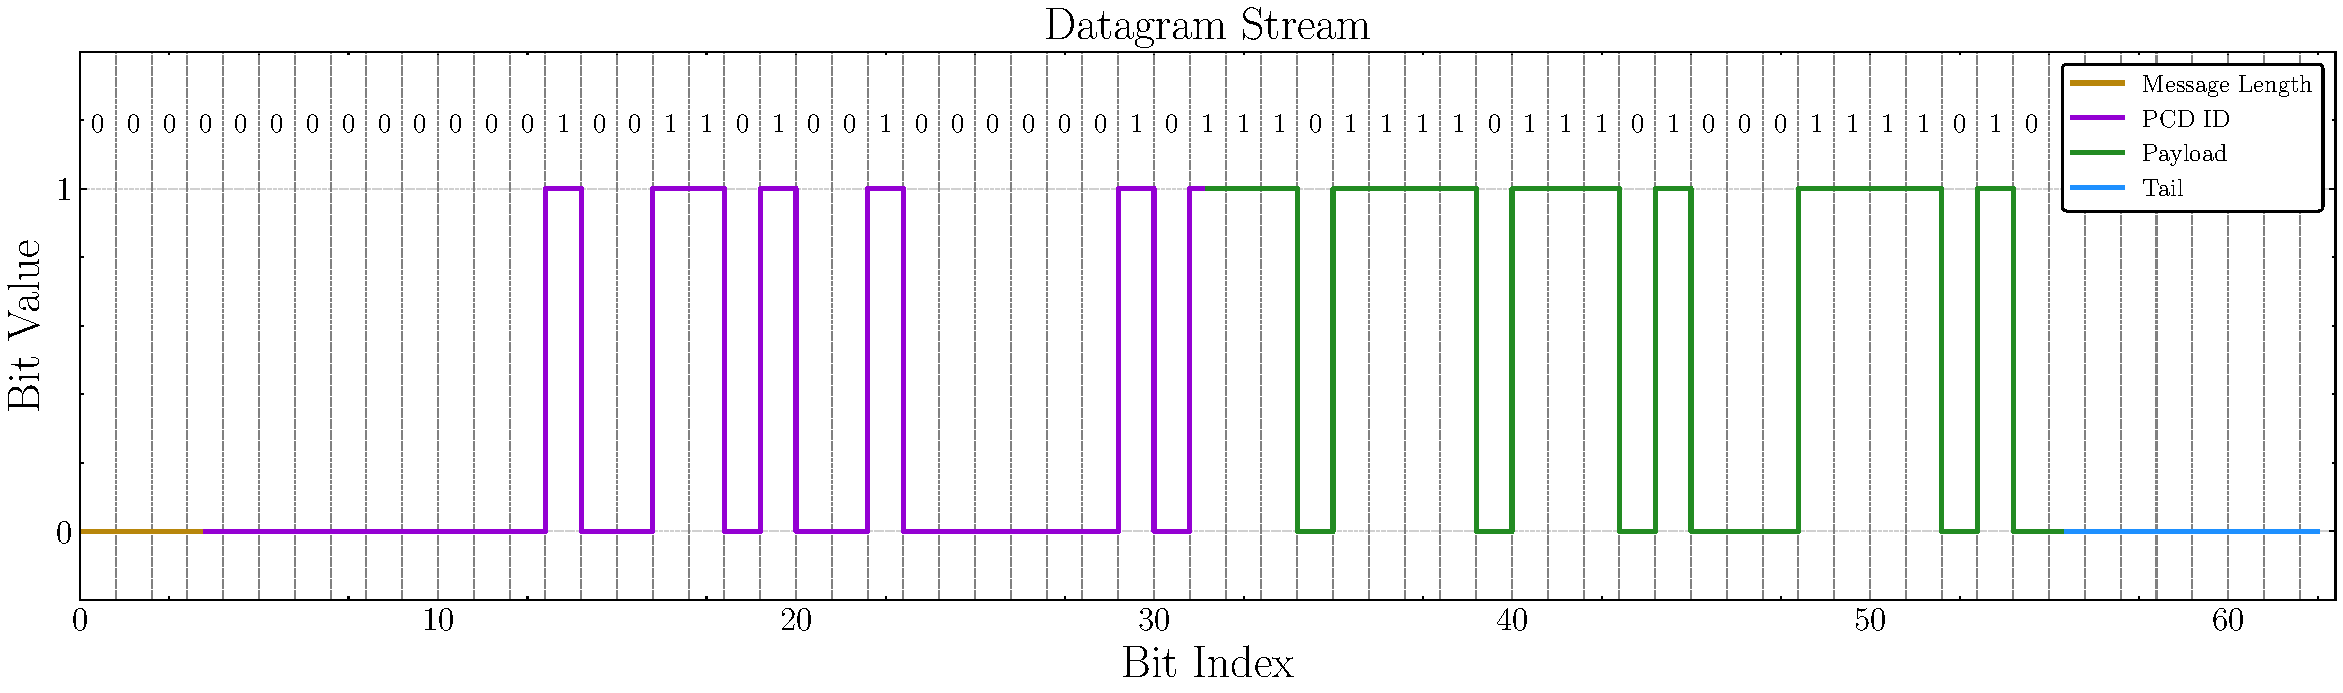
\includegraphics[width=\linewidth]{assets/cap3/transmitter_datagram_time.pdf}
\end{figure}

Após a montagem dos bits \gls{ut} do datagrama, os mesmos são codificados utilizando codificação convolucional, conforme detalhado na seção \ref{sec:conv_coding}, resultando nos vetores de bits \gls{vt0} e \gls{vt1}, que por sua vez são embaralhados resultando nas sequências \gls{Xn} e \gls{Yn} para os canais \gls{cI} e \gls{cQ}, respectivamente, o processo de codificação convolucional aplicado no vetor \gls{ut} é ilustrado na \autoref{fig:transmitter_conv_time}.

\begin{figure}[H]
	\centering
	\caption{Codificação convolucional do datagrama ARGOS-3}\label{fig:transmitter_conv_time}
	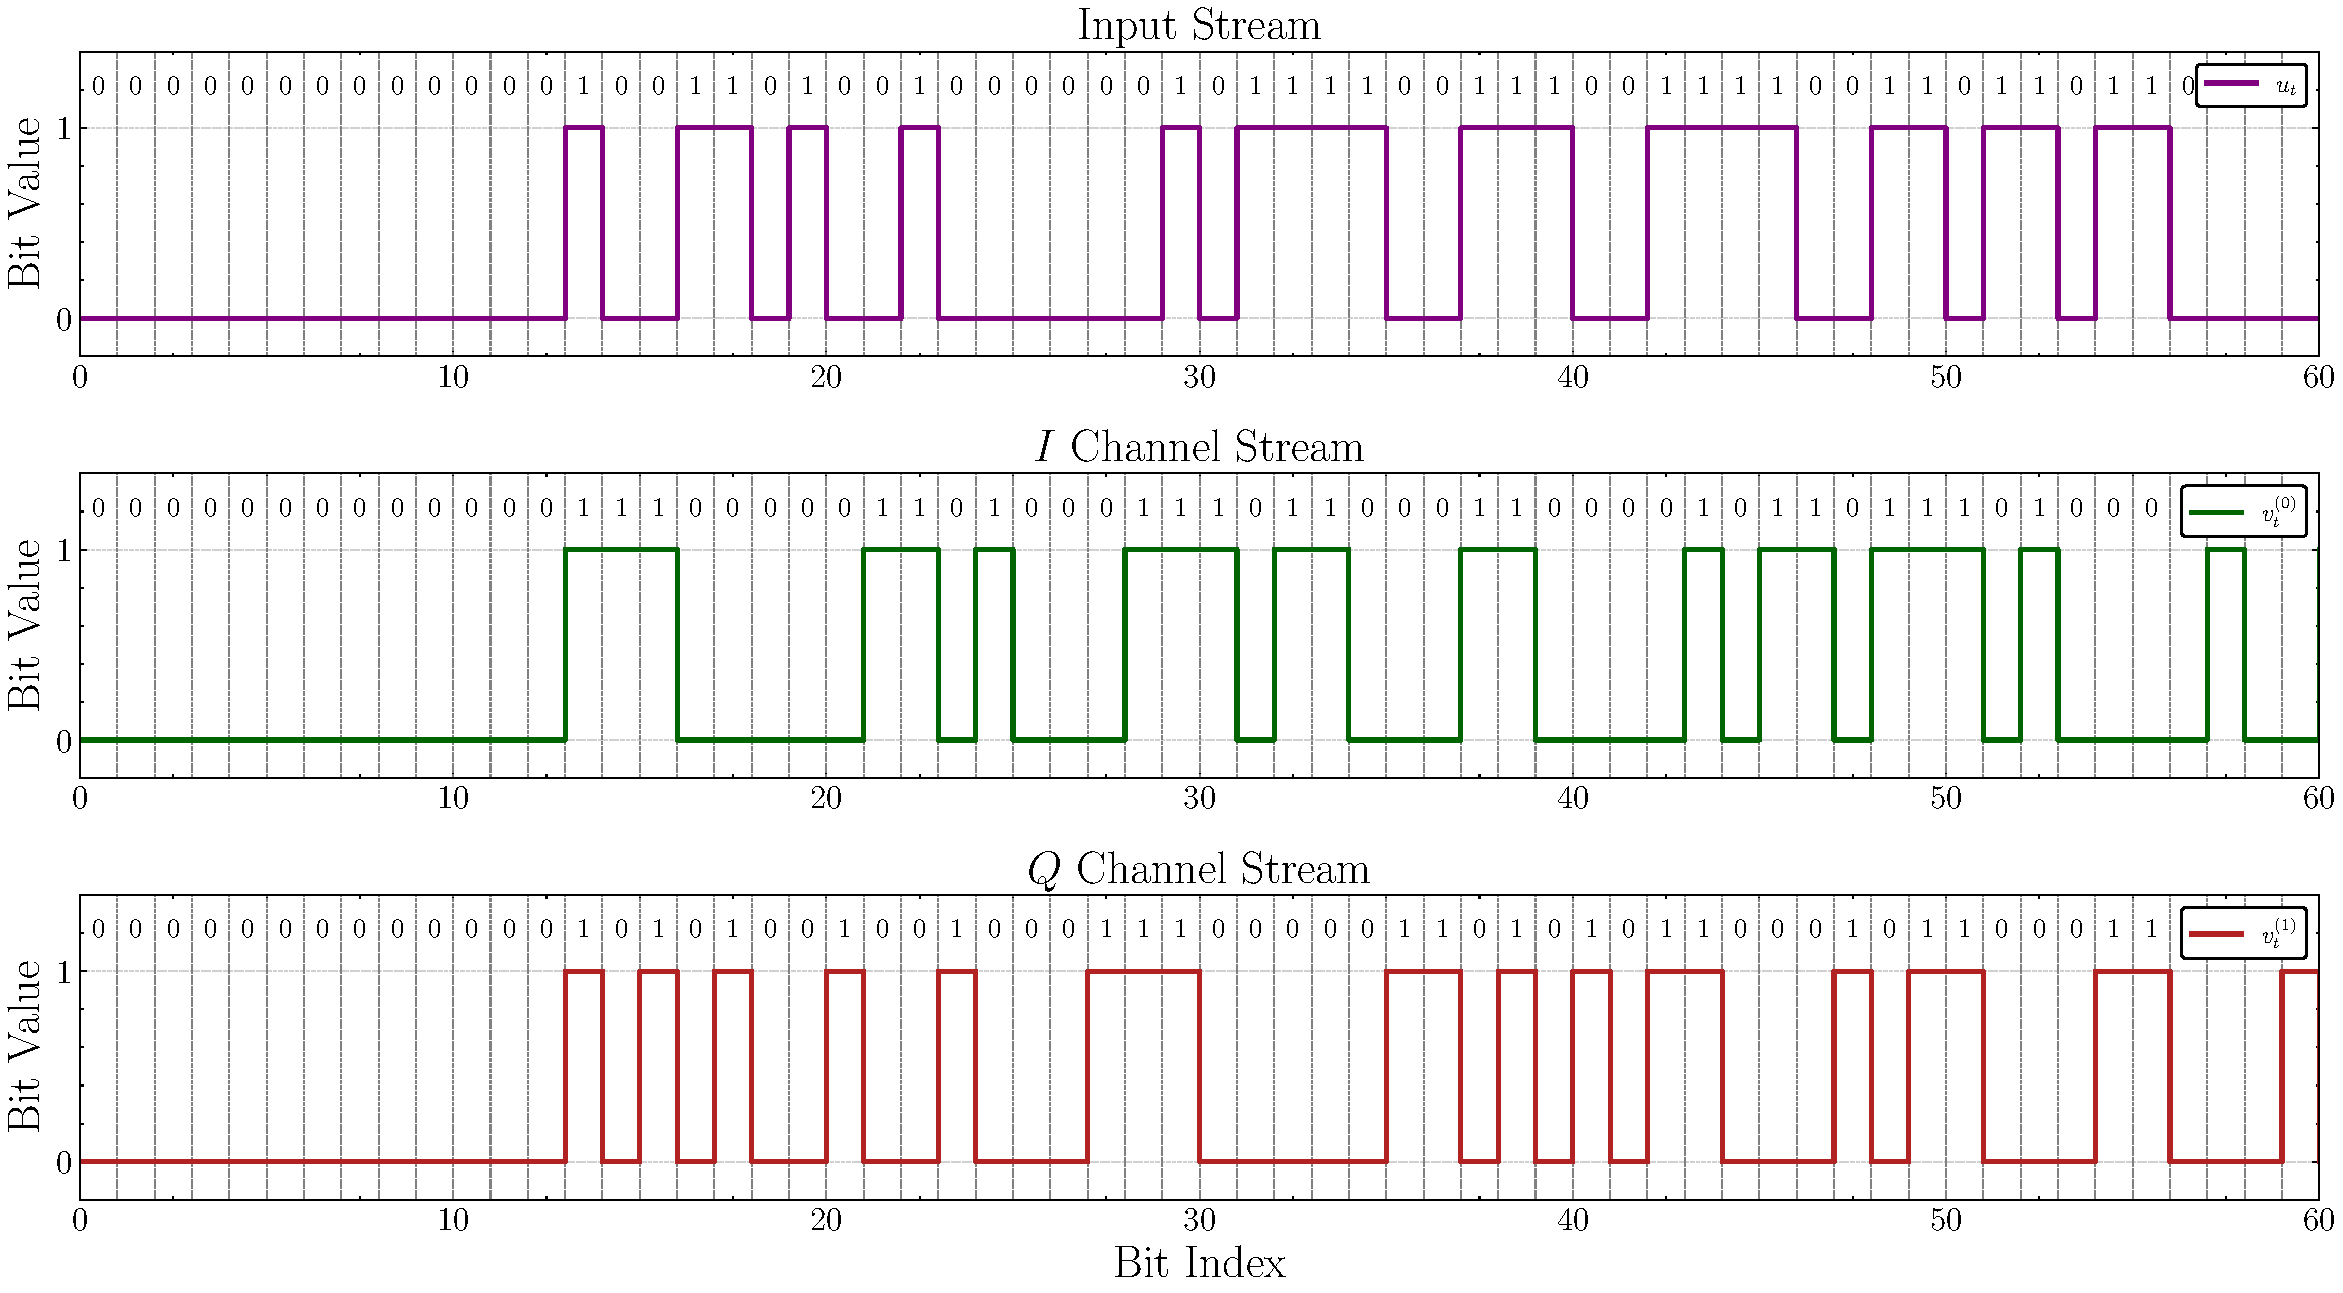
\includegraphics[width=\linewidth]{assets/cap3/transmitter_conv_time.pdf}
\end{figure}

As sequências \gls{Xn} e \gls{Yn} já embaralhadas, são então multiplexadas com o preâmbulo \gls{SIn} e \gls{SQn} dos canais \gls{cI} e \gls{cQ} respectivamente, gerados conforme apresentado na seção \ref{sec:preambulo}. A adição das sequências é fundamental para permitir a sincronização de símbolos no receptor, esse processo é ilustrado na \autoref{fig:mux_time} abaixo.

\begin{figure}[H]
	\centering
	\caption{Multiplexação com preâmbulo}\label{fig:mux_time}
	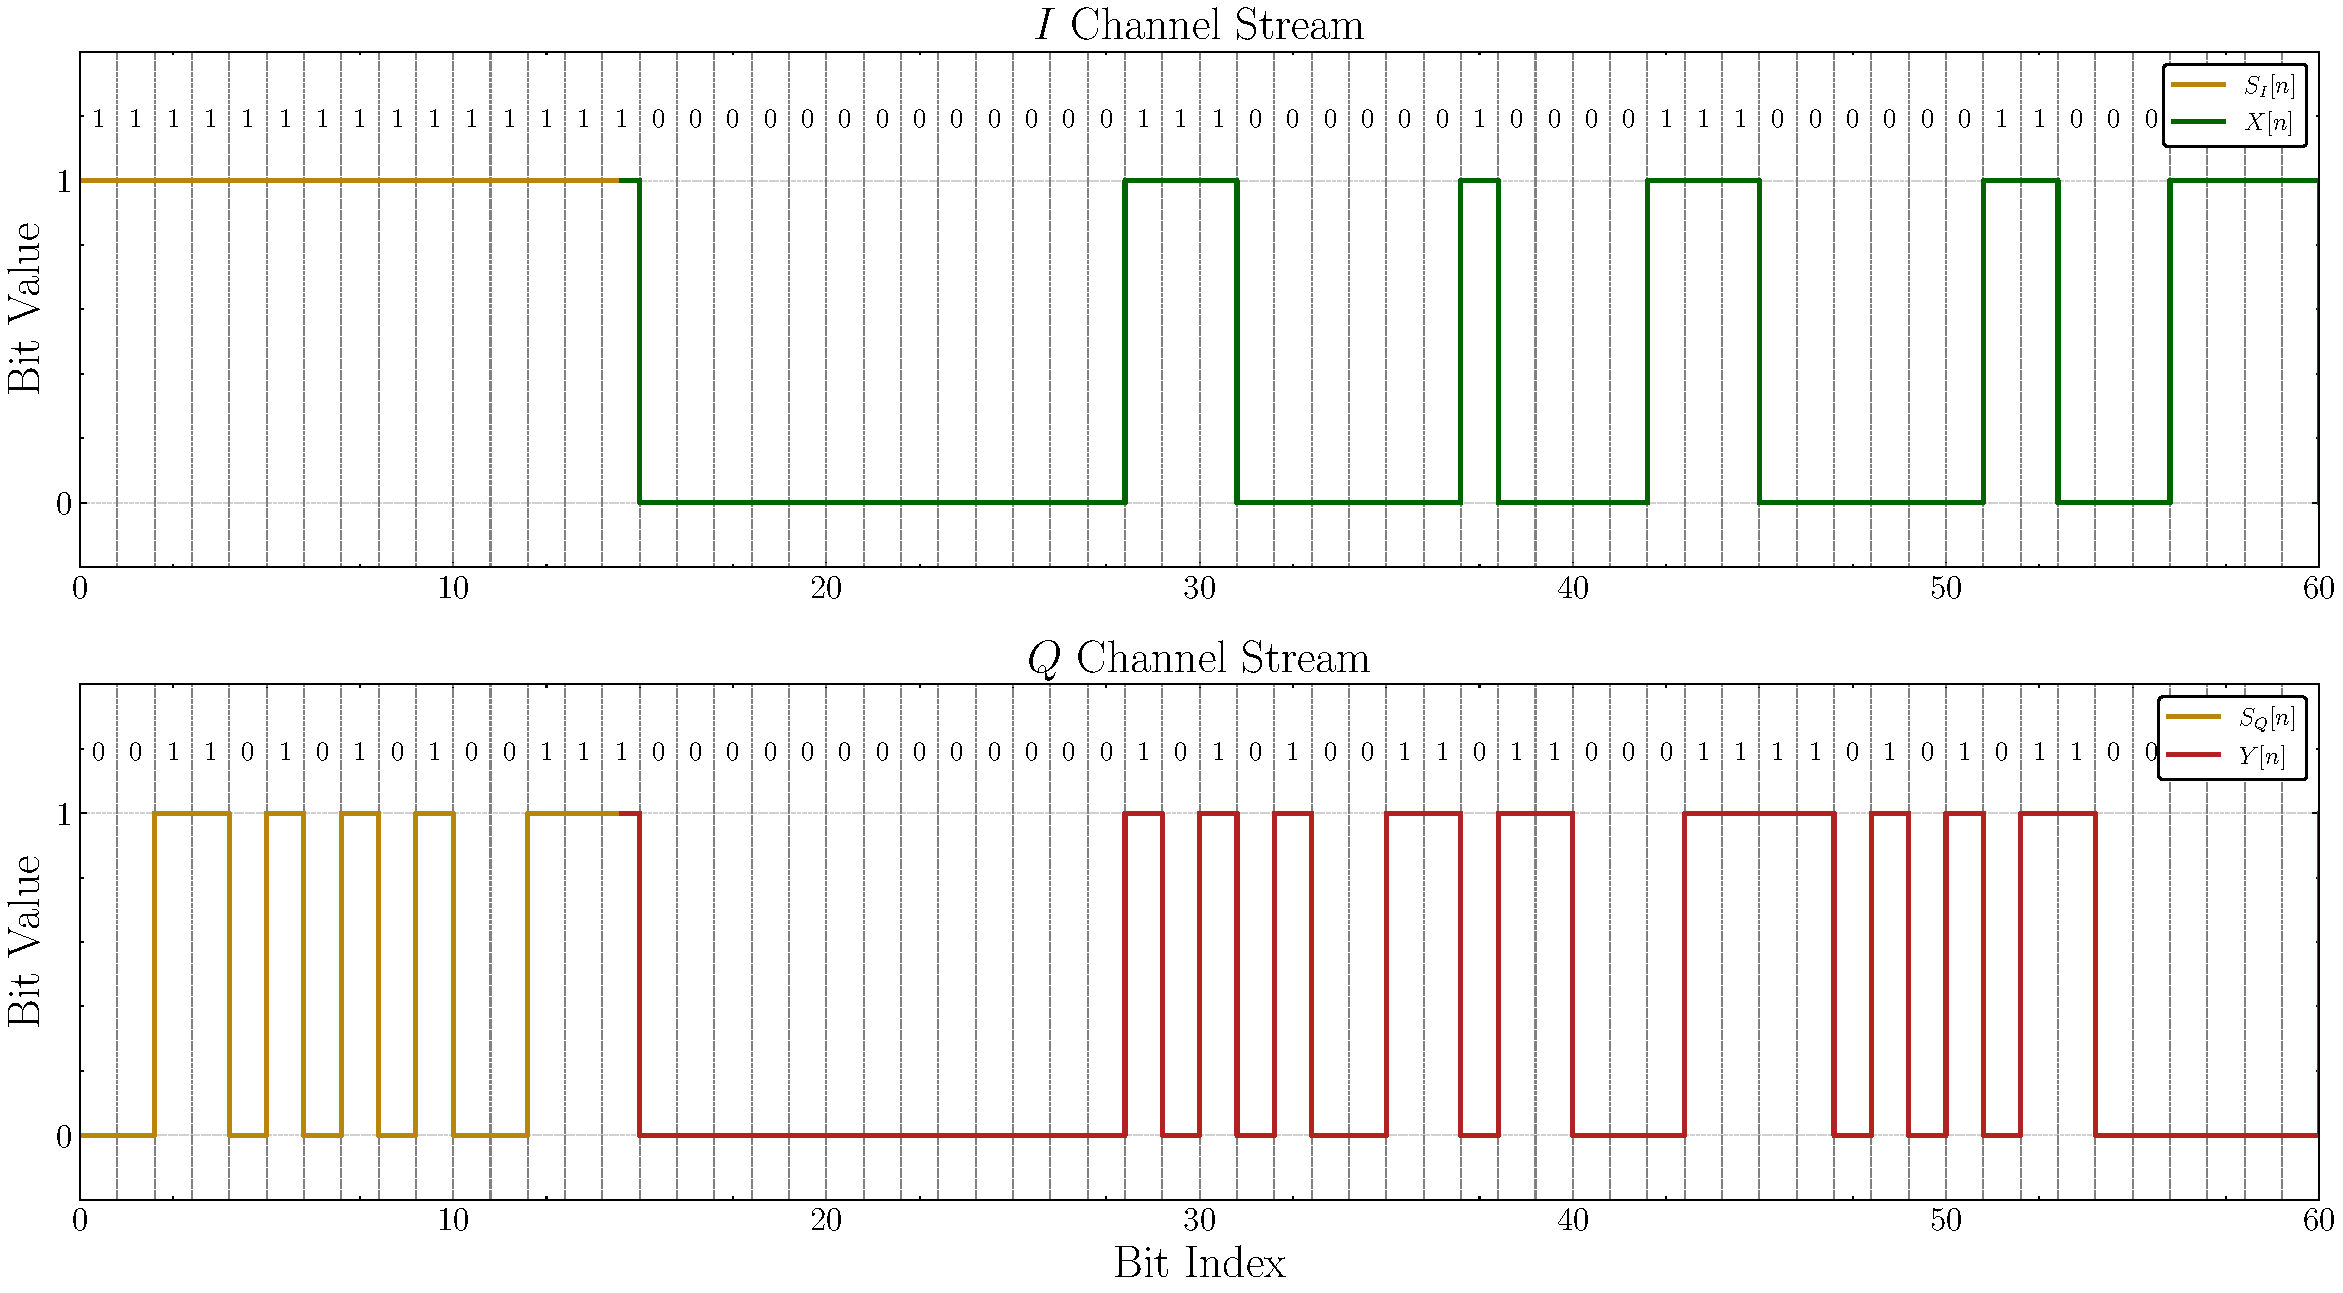
\includegraphics[width=\linewidth]{assets/cap3/transmitter_mux_time.pdf}
\end{figure}

Em seguida, os bits são codificados utilizando codificação de linha para melhorar as características espectrais do sinal modulado, como detalhado na seção \ref{sec:line_coding}, neste processo é utilizado apenas codificação \gls{NRZ} para os dois canais, pois a técnica \gls{Manchester} será aplicada posteriormente na modulação de pulso do canal \gls{cQ}, o processo de codificação de linha de ambos os canais é ilustrado na \autoref{fig:encoder_time}.

\begin{figure}[H]
	\centering
	\caption{Codificação de linha}\label{fig:encoder_time}
	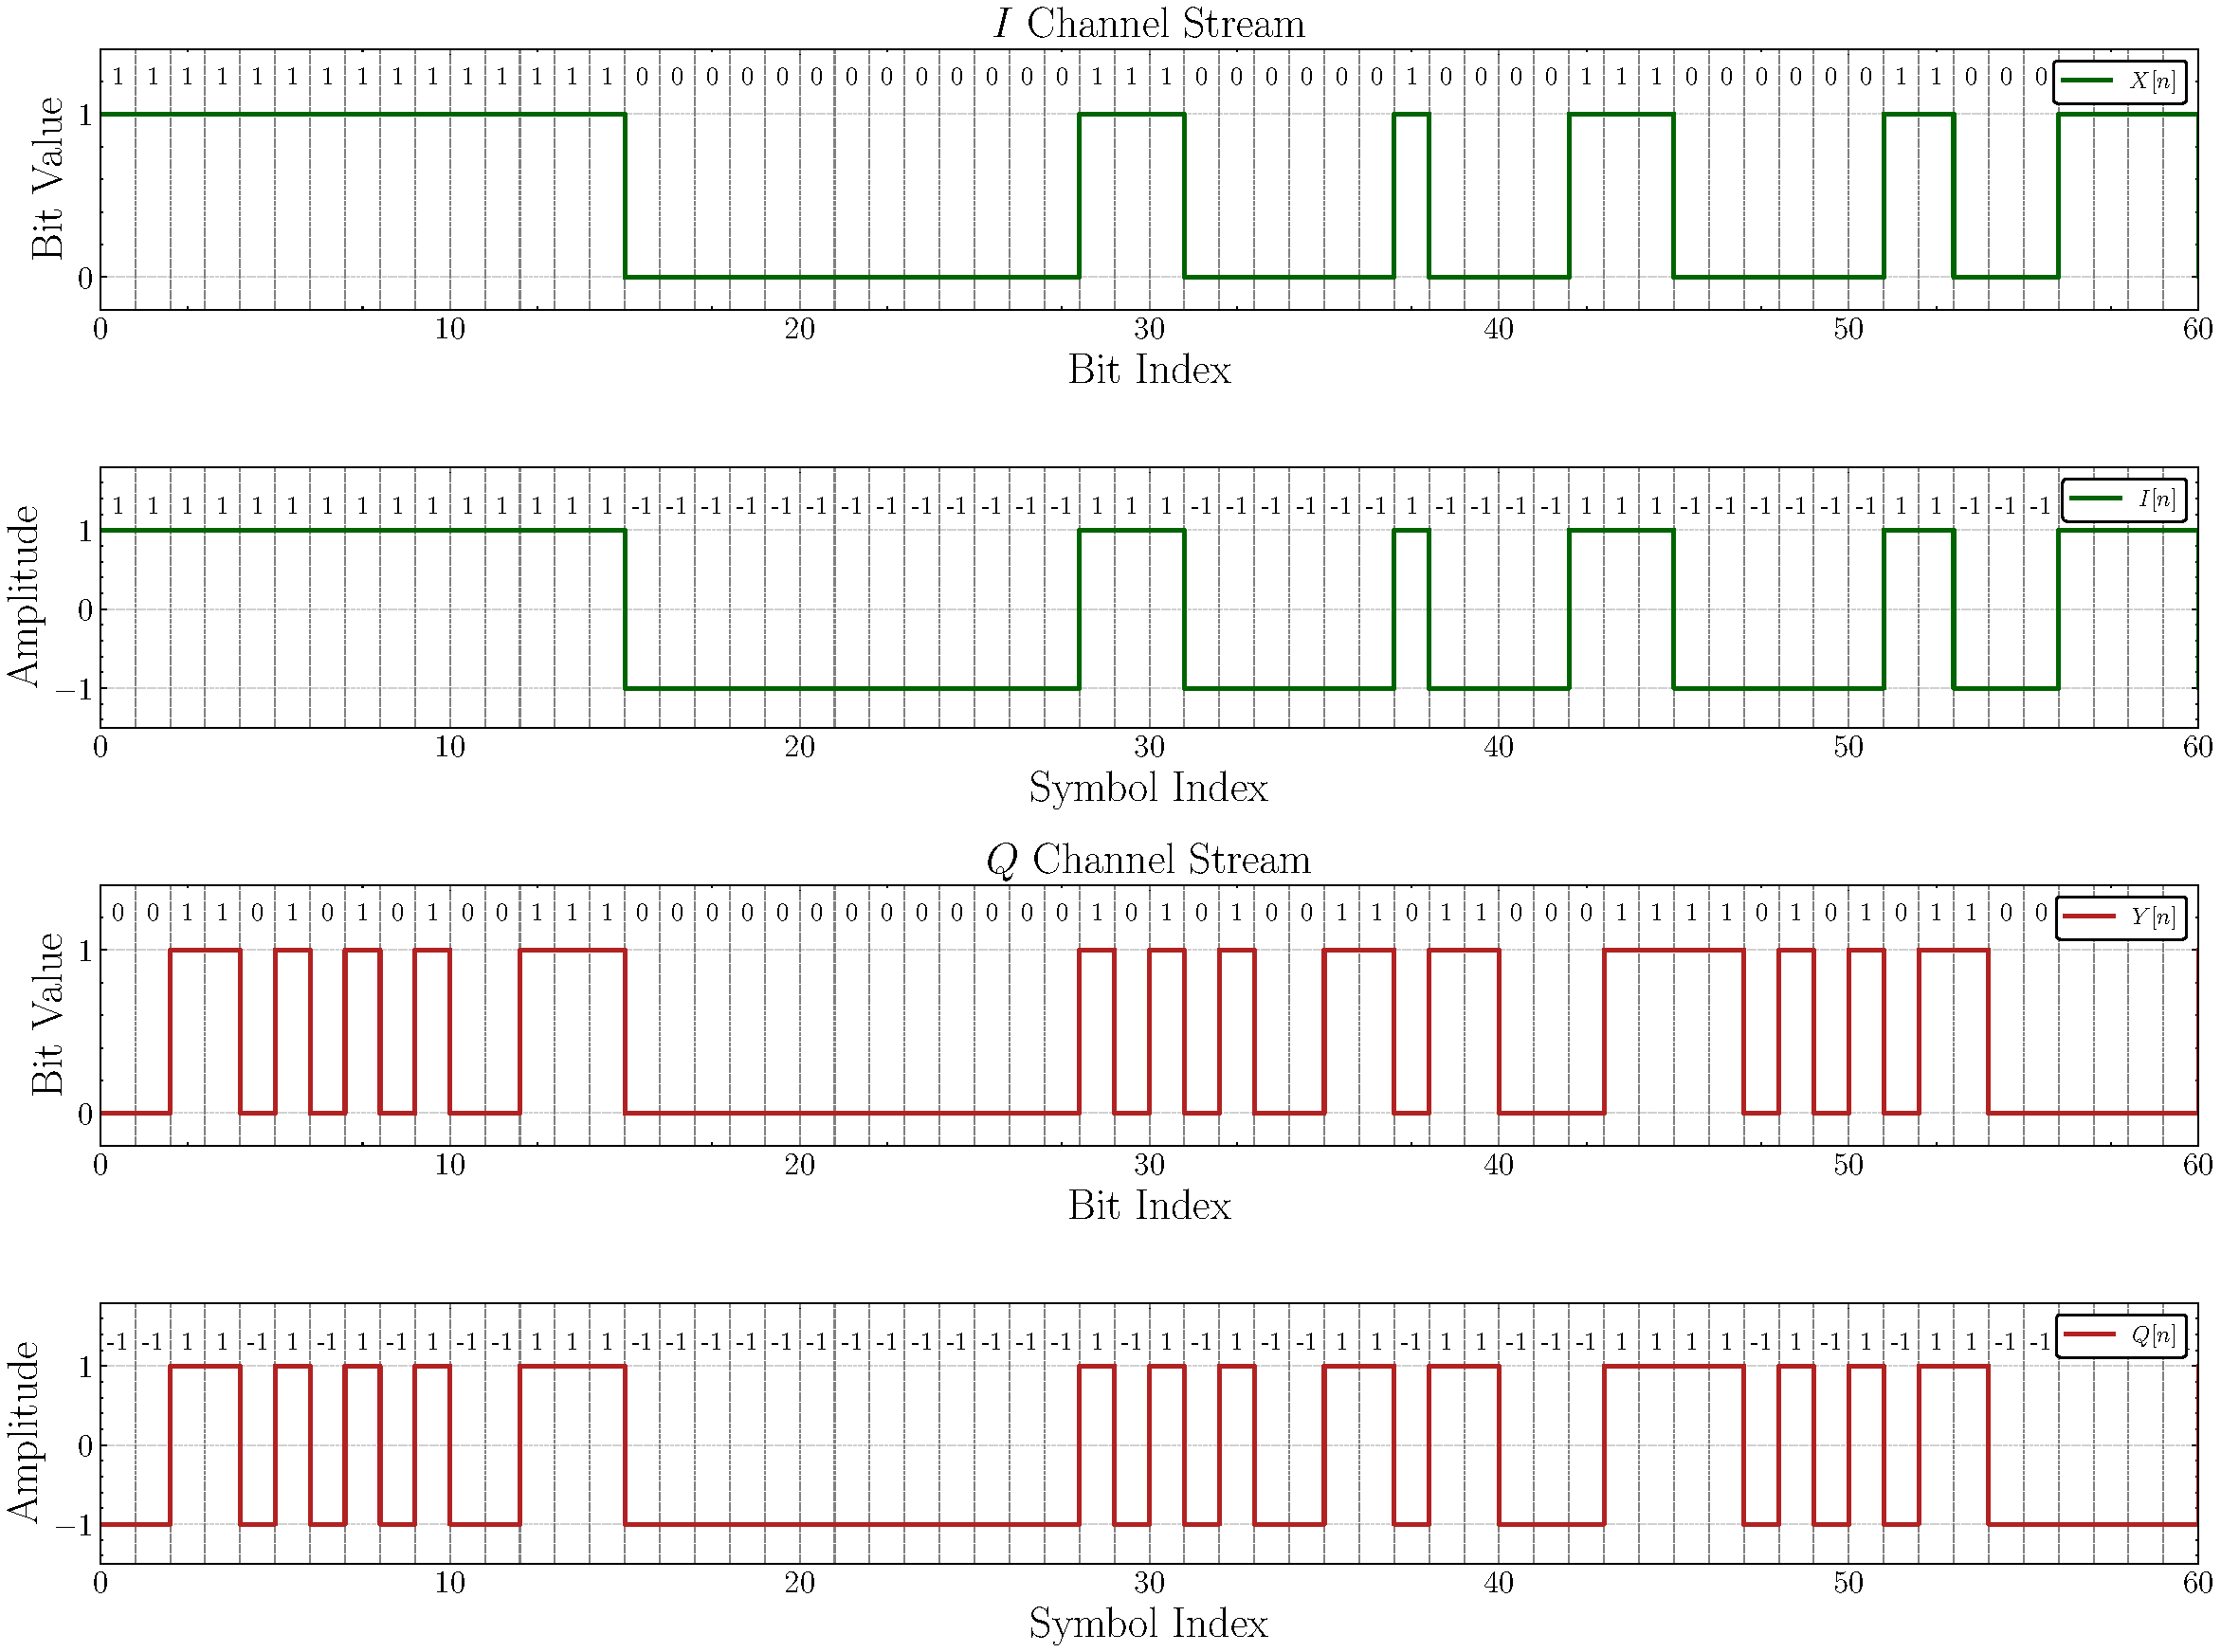
\includegraphics[width=\linewidth]{assets/cap3/transmitter_encoder_time.pdf}
\end{figure}

As sequências de simbolos \gls{In} e \gls{Qn} resultantes da codificação de linha, estão prontas para serem moduladas utilizando modulação de pulso. 

\subsection{Modulação de pulso RRC e Manchester}

Após a montagem das sequências de simbolos \gls{In} e \gls{Qn}, o próximo passo é a modulação de pulso, onde o canal \gls{cI} utiliza um filtro de pulso \gls{RRC} e o canal \gls{cQ} utiliza um filtro de pulso \gls{Manchester}, conforme detalhado na seção \ref{sec:line_coding}. A modulação de pulso é fundamental para reduzir a largura de banda \gls{W} do sinal que está sendo transmitido e também reduzir a interferência entre símbolos \gls{ISI}. O processo de modulação de pulso dos canais \gls{cI} e \gls{cQ} é ilustrado na \autoref{fig:pulse_modulate_diagram}.

\begin{figure}[H]
    \centering
    \caption{Diagrama de blocos do modulador de pulso para os canais $I$ e $Q$}\label{fig:pulse_modulate_diagram}
    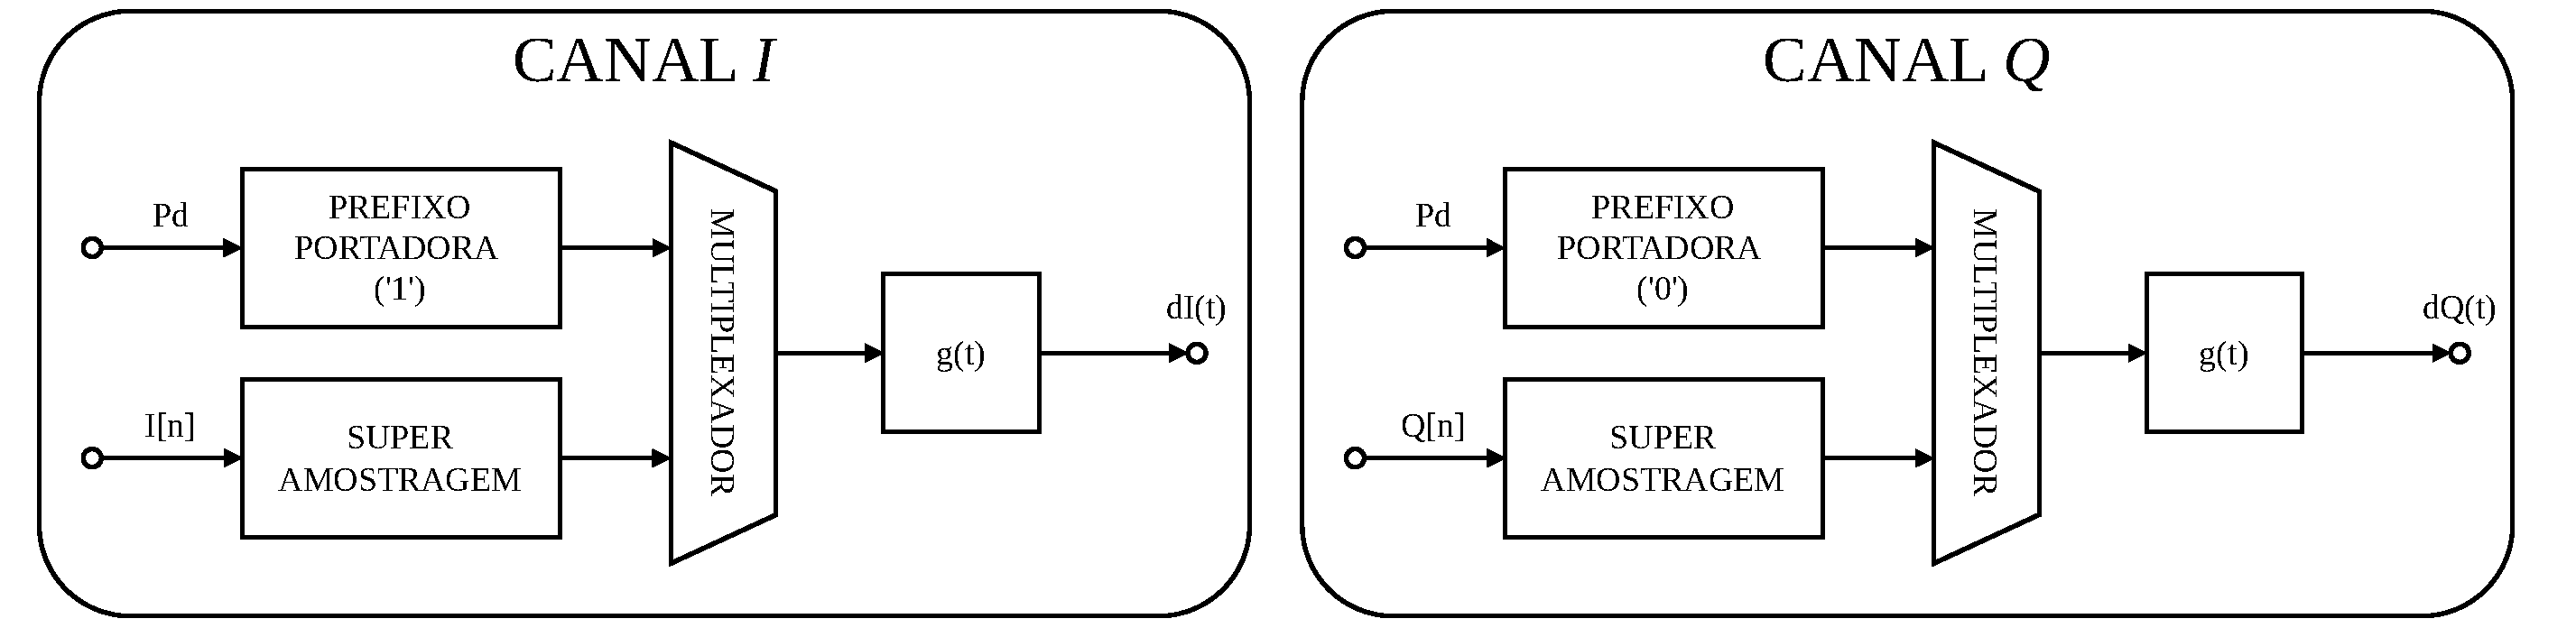
\includegraphics[width=\linewidth]{assets/diagrams/pulse_modulate.pdf}
\end{figure}

\subsubsection{Pulso RRC e Manchester}

Antes de aplicar a modulação de pulso, é necessário gerar os filtros de pulso \gls{RRC} e \gls{Manchester}, que serão utilizados para modular os canais \gls{cI} e \gls{cQ}, respectivamente. A resposta ao impulso do filtro \gls{RRC} é ilustrada na \autoref{fig:impulse_response_rrc}, e é calculada conforme apresentado na seção \ref{sec:pulse_modulation}. 

\begin{figure}[H]
	\centering
	\caption{Resposta ao impulso - Pulso RRC}\label{fig:impulse_response_rrc}
	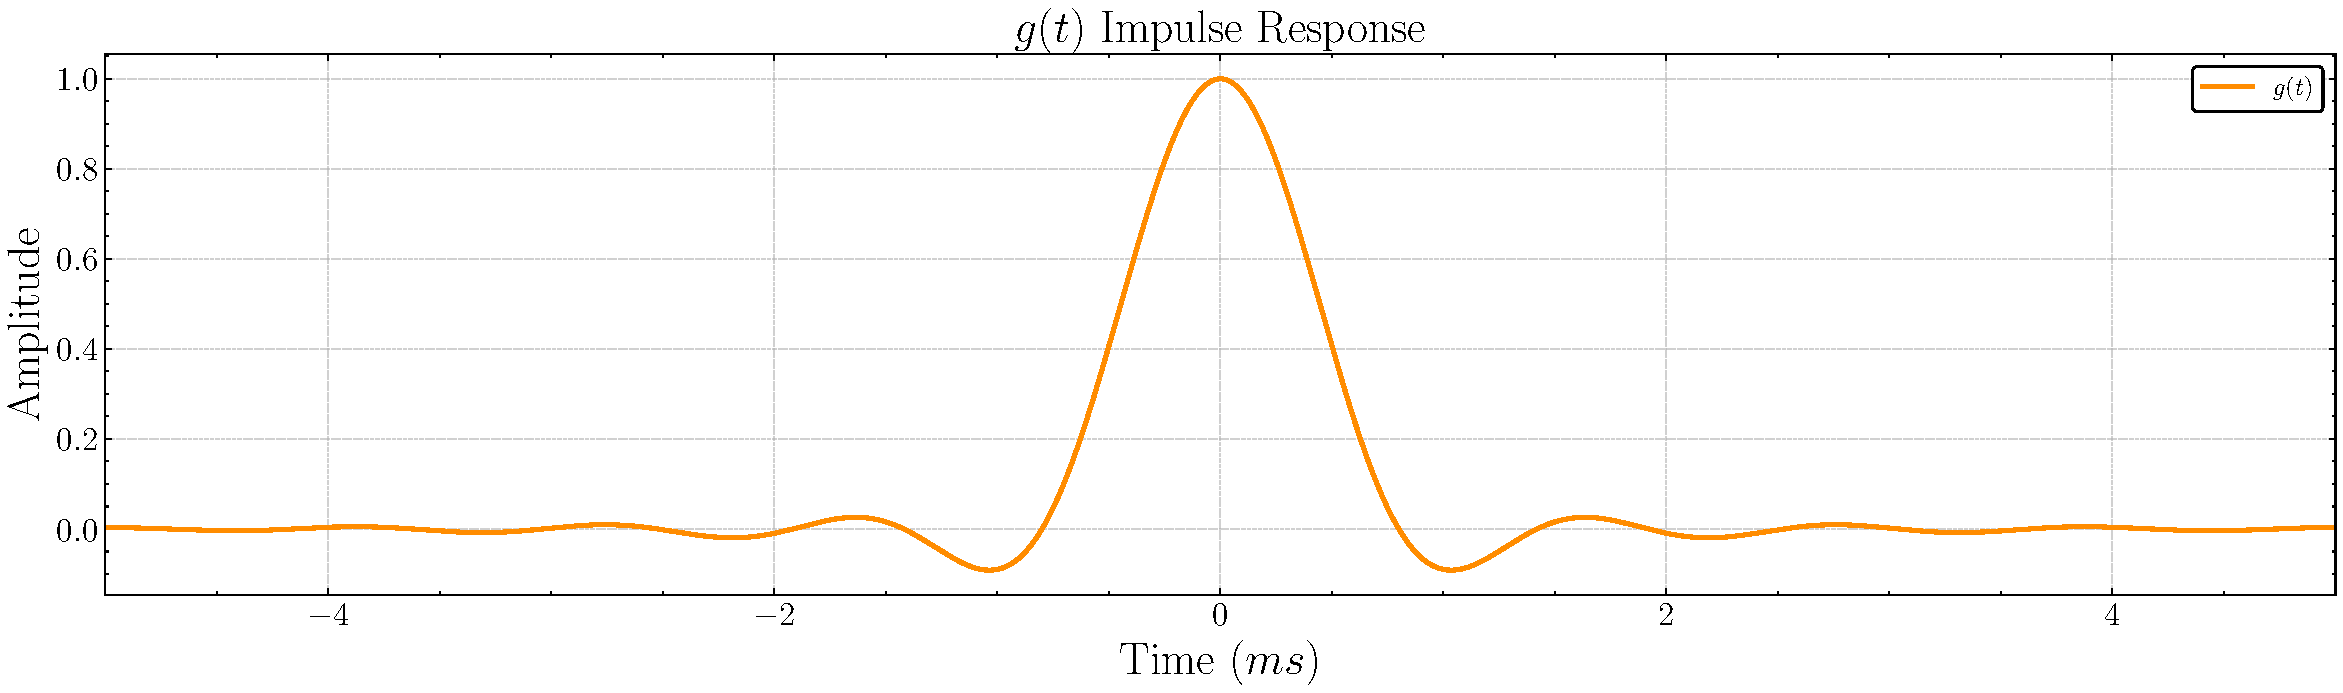
\includegraphics[width=\linewidth]{assets/cap3/example_formatter_impulse.pdf}
\end{figure}

Já o pulso \gls{Manchester} é gerado através de uma soma de dois pulsos \gls{RRC} deslocados no tempo, um positivo deslocado em $T_b/2$ e outro negativo deslocado em $-T_b/2$, conforme ilustrado na \autoref{fig:impulse_response_man}. O calculo do pulso pode ser expresso como 

\begin{equation}
g_{MAN}(t) = g_{RRC}(t + T_b/2) - g_{RRC}(t - T_b/2)
\end{equation}

Onde $g_{MAN}(t)$ é o pulso Manchester, $g_{RRC}(t)$ é o pulso RRC e $T_b$ é o tempo de bit. A resposta ao impulso do filtro \gls{Manchester} é ilustrada na \autoref{fig:impulse_response_man}.

\begin{figure}[H]
	\centering
	\caption{Resposta ao impulso - Pulso Manchester}\label{fig:impulse_response_man}
	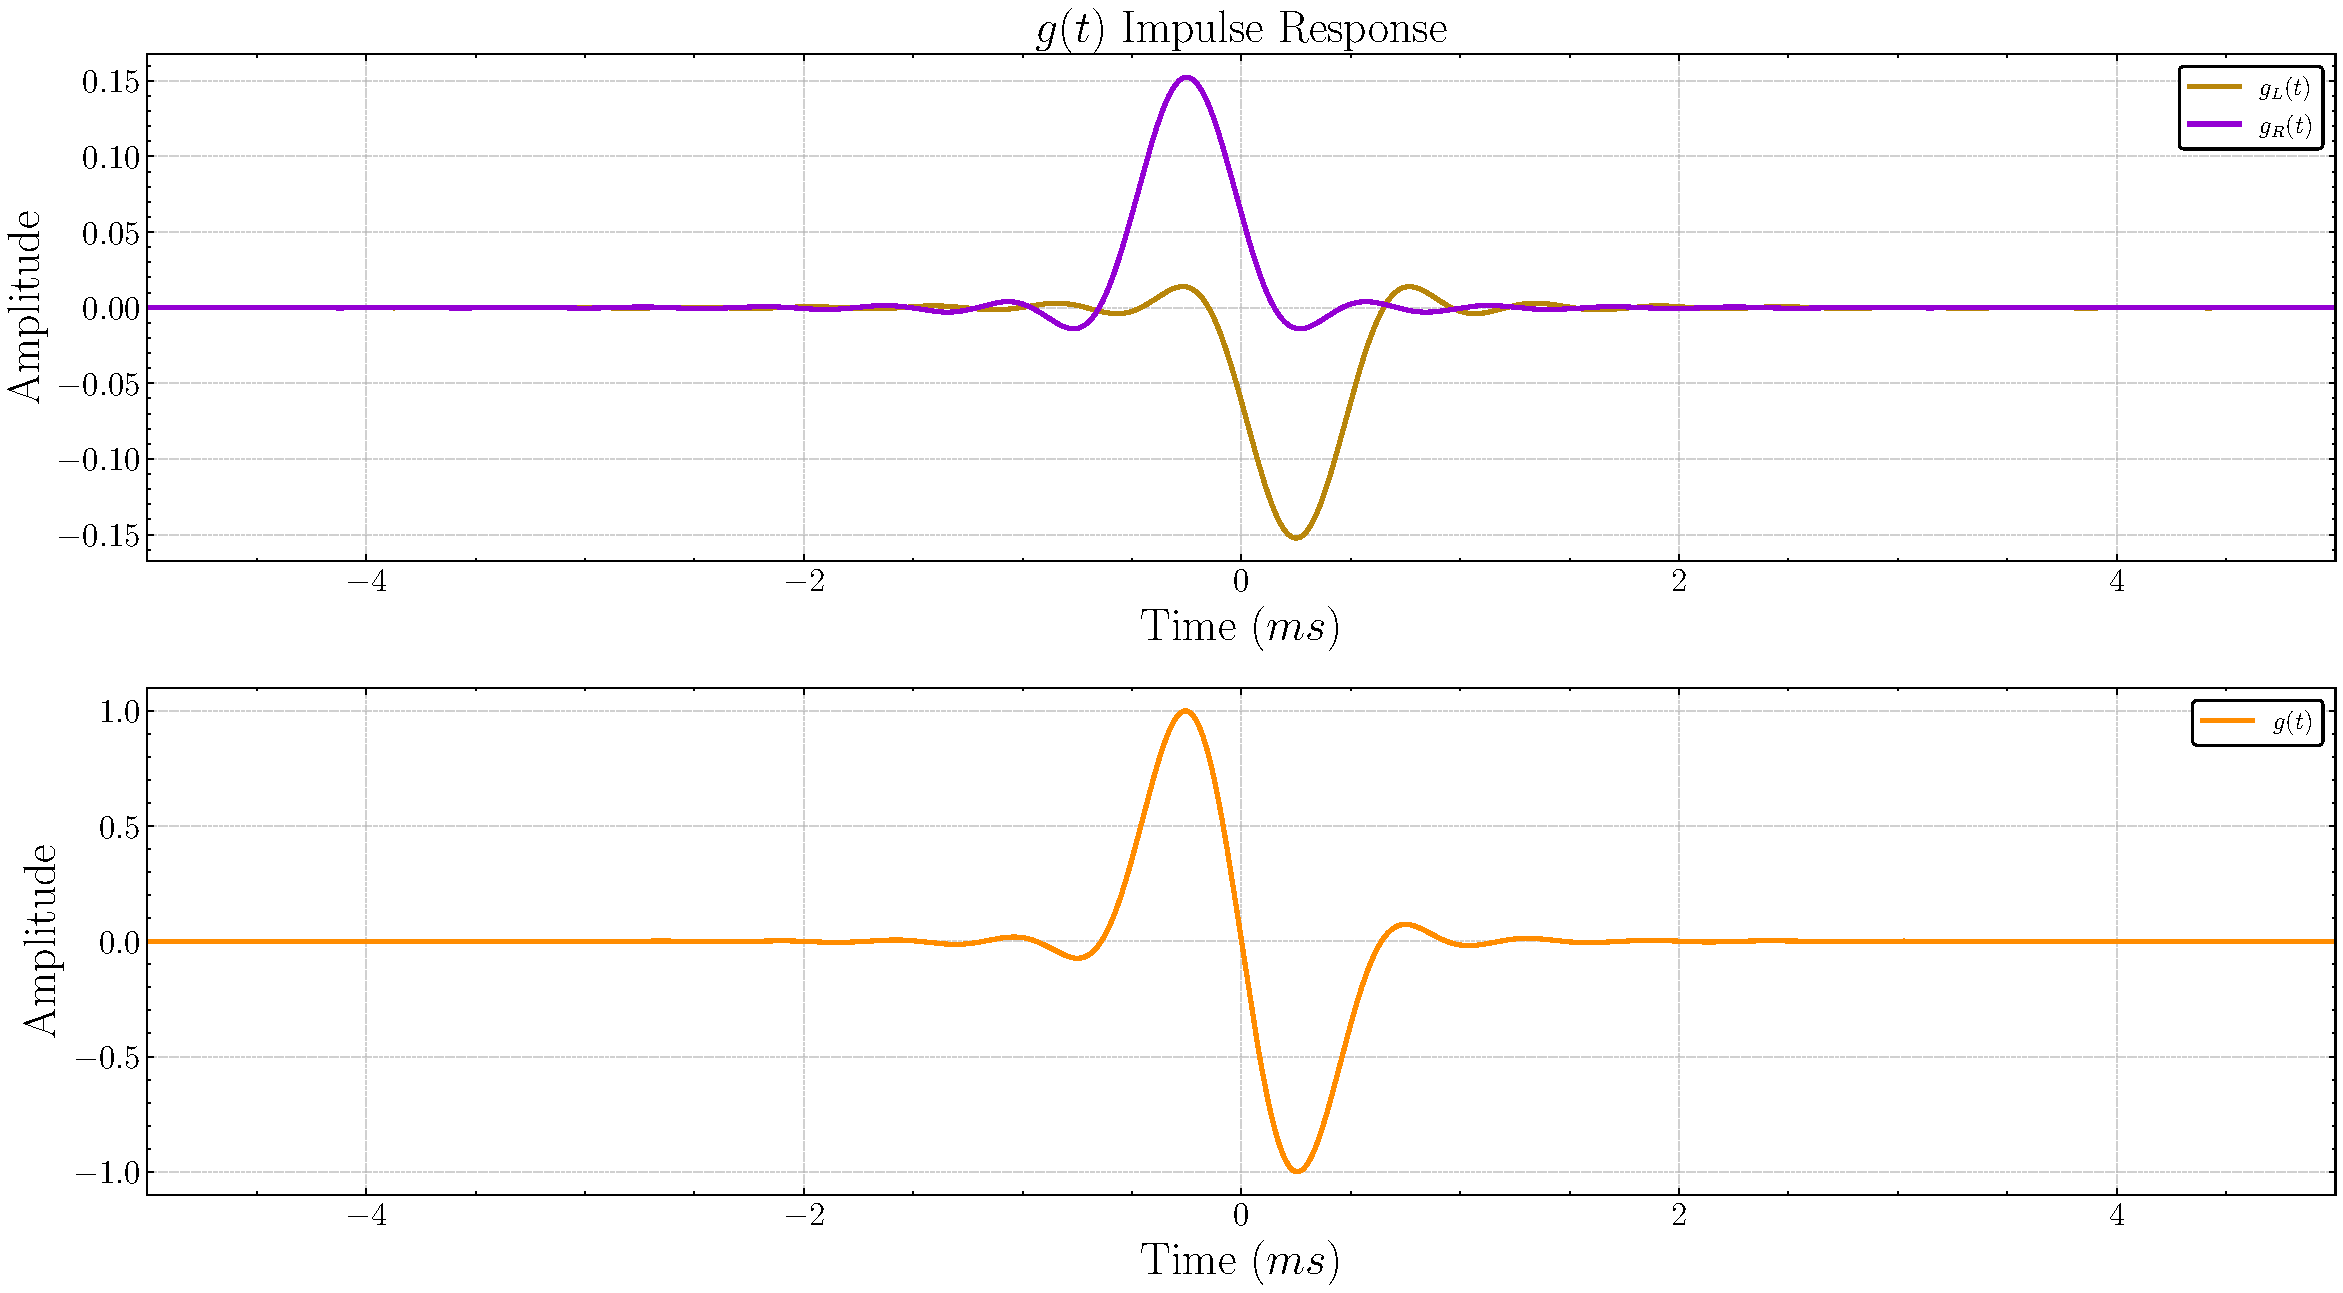
\includegraphics[width=\linewidth]{assets/cap3/example_formatter_impulse_man.pdf}
\end{figure}

A utilização do pulso \gls{Manchester} no canal \gls{cQ} ao invés da codificação de linha \gls{Manchester} proposta originalmente tem como objetivo simplificar a implementação do sistema, reduzindo a complexidade computacional e o número de etapas necessárias na cadeia de transmissão. 

\subsubsection{Modulação de pulso dos canais I e Q}

Uma vez com os filtros de pulso \gls{RRC} e \gls{Manchester} gerados, é possível aplicar a modulação de pulso nos canais \gls{cI} e \gls{cQ}, respectivamente gerando os sinais \gls{dI} e \gls{dQ} modulados em banda base. Esse processo envolve a superamostragem dos vetores de simbolos \gls{In} e \gls{Qn}, em função da frequência de amostragem \gls{fs}, seguida da filtragem com os respectivos filtros de pulso. 

O resultado são as sequências \gls{dI} e \gls{dQ} contínuas ao longo do tempo \gls{t}, onde cada bit de informação é transmitido durante um período de tempo $\text{ \gls{Tb}} = 1/ \text{\gls{Rb}}$ (tempo de bit), definido com base na taxa de bit \gls{Rb}. A modulação de pulso dos canais \gls{cI} e \gls{cQ} é ilustrada na \autoref{fig:transmitter_formatter_time}.

\begin{figure}[H]
	\centering
	\caption{Modulação de pulso dos canais $I$ e $Q$}\label{fig:transmitter_formatter_time}
	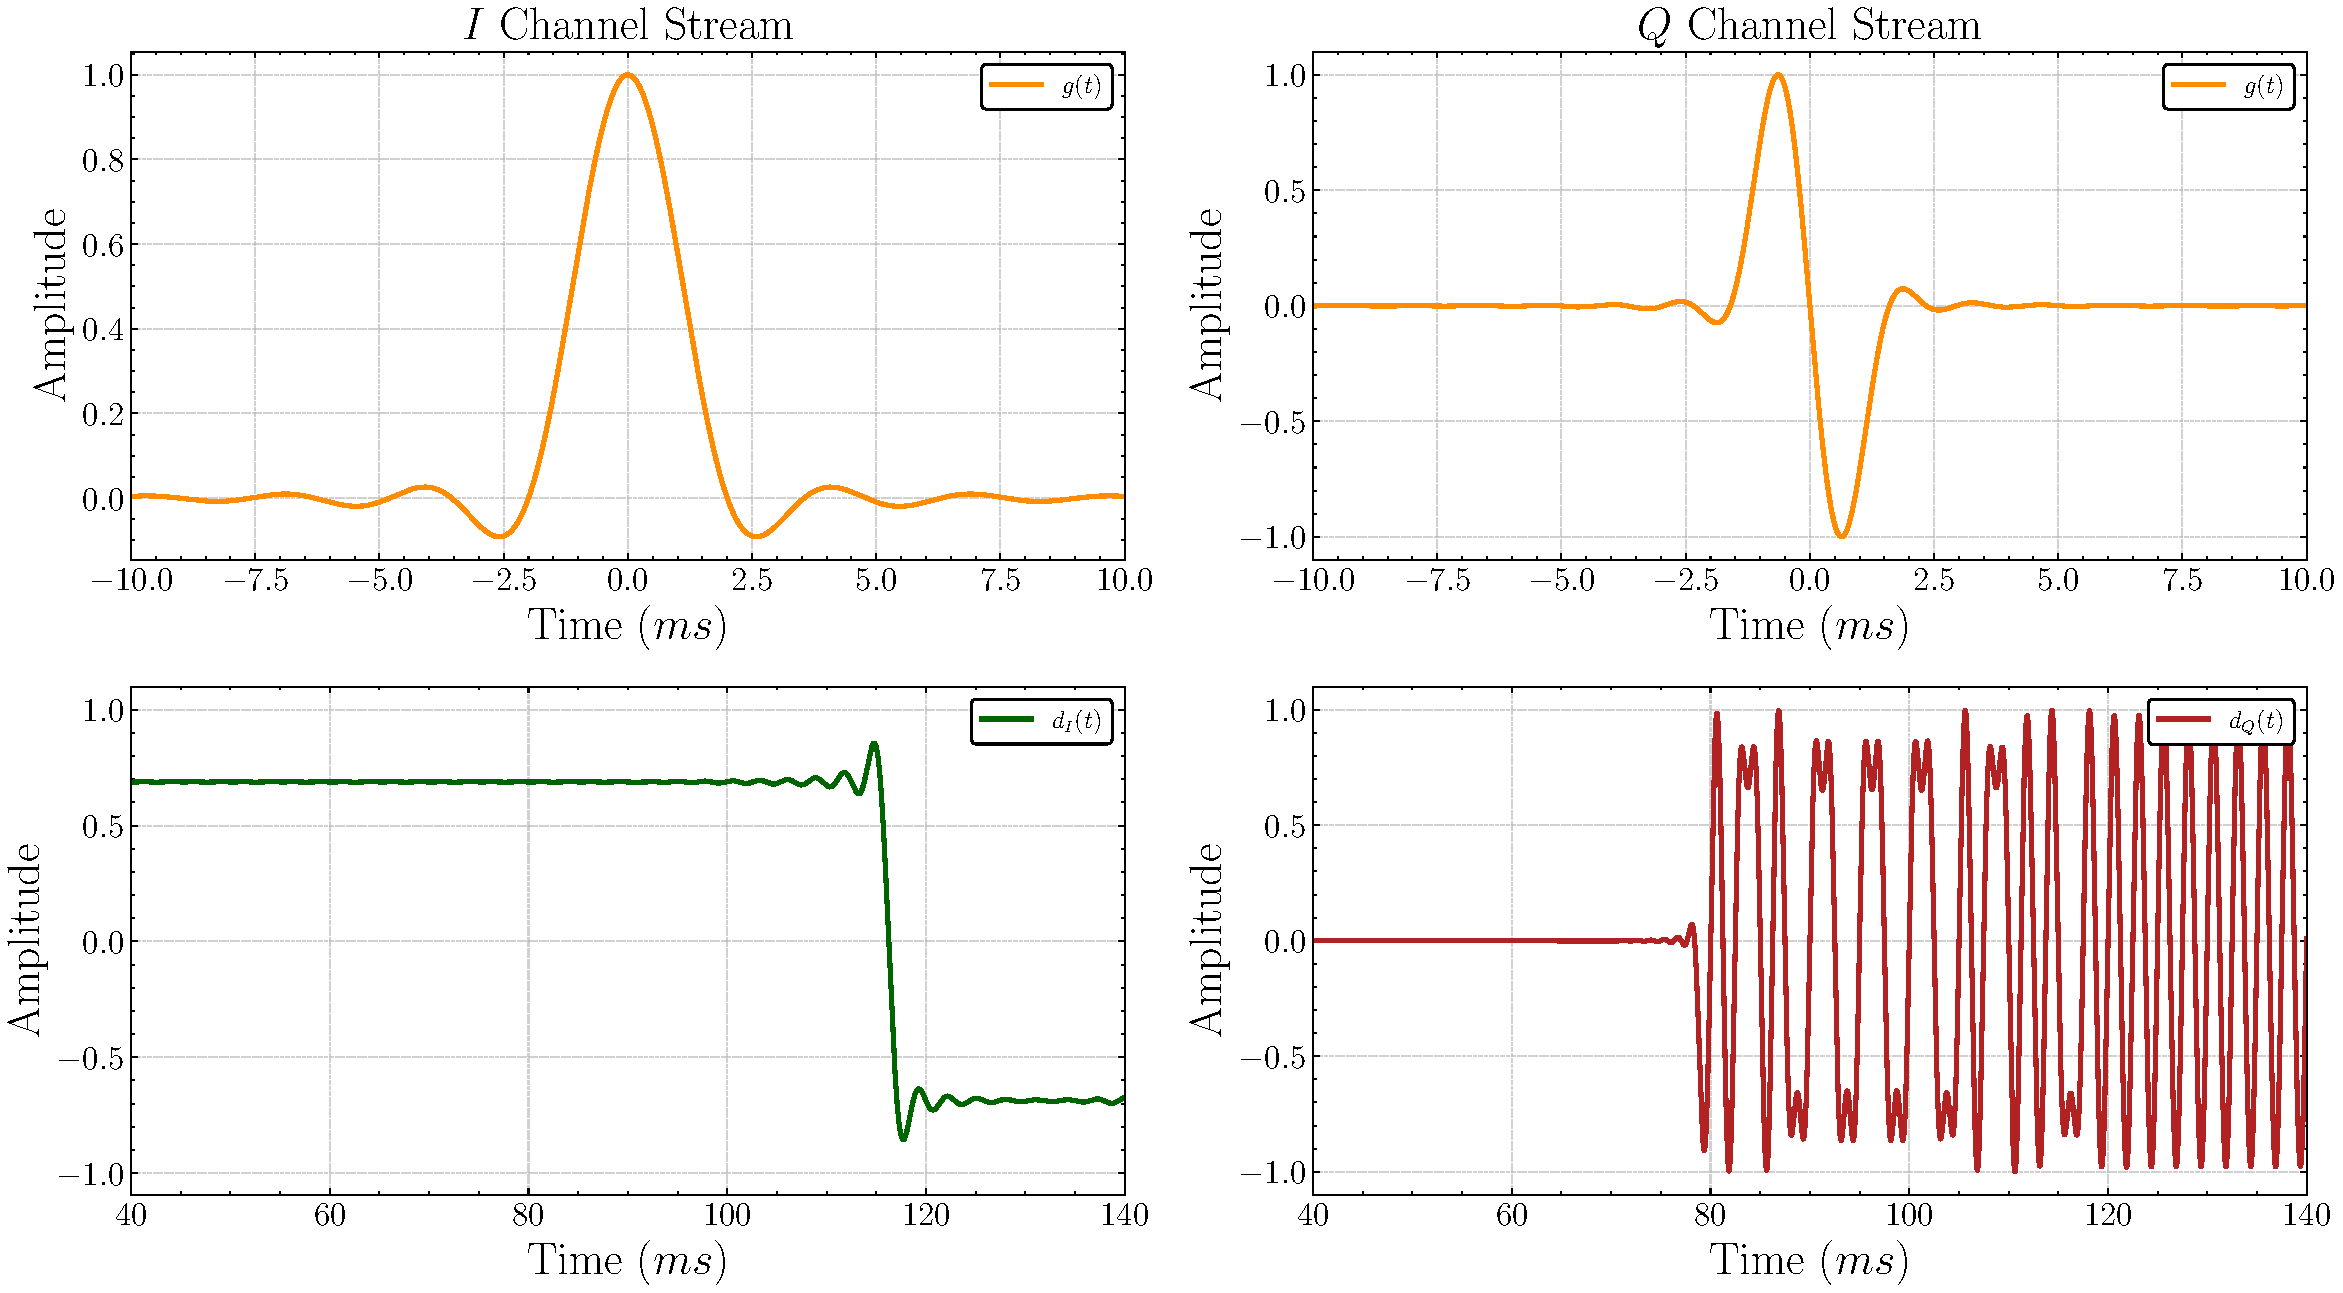
\includegraphics[width=\linewidth]{assets/cap3/transmitter_formatter_time.pdf}
\end{figure}

As sequências \gls{dI} e \gls{dQ} estão agora prontas para serem moduladas em banda passante utilizando modulação em fase em quadratura (\gls{QPSK}), conforme detalhado na seção \ref{sec:qpsk}.

\subsection{Modulação em fase em quadratura (QPSK)}\label{sec:qpsk}

Na modulação \gls{QPSK}, os sinais modulados em banda base \gls{dI} e \gls{dQ} são utilizados para modular uma componente senoideal e uma componente cossenoidal, respectivamente, com frequência \gls{fc}, o somatório dessas duas componentes moduladas resulta no sinal modulado em banda passante \gls{st}, conforme ilustrado na \autoref{fig:transmitter_modulator_time}.

\begin{figure}[H]
	\centering
	\caption{Modulação em banda passante canais $I$ e $Q$}\label{fig:transmitter_modulator_time}
	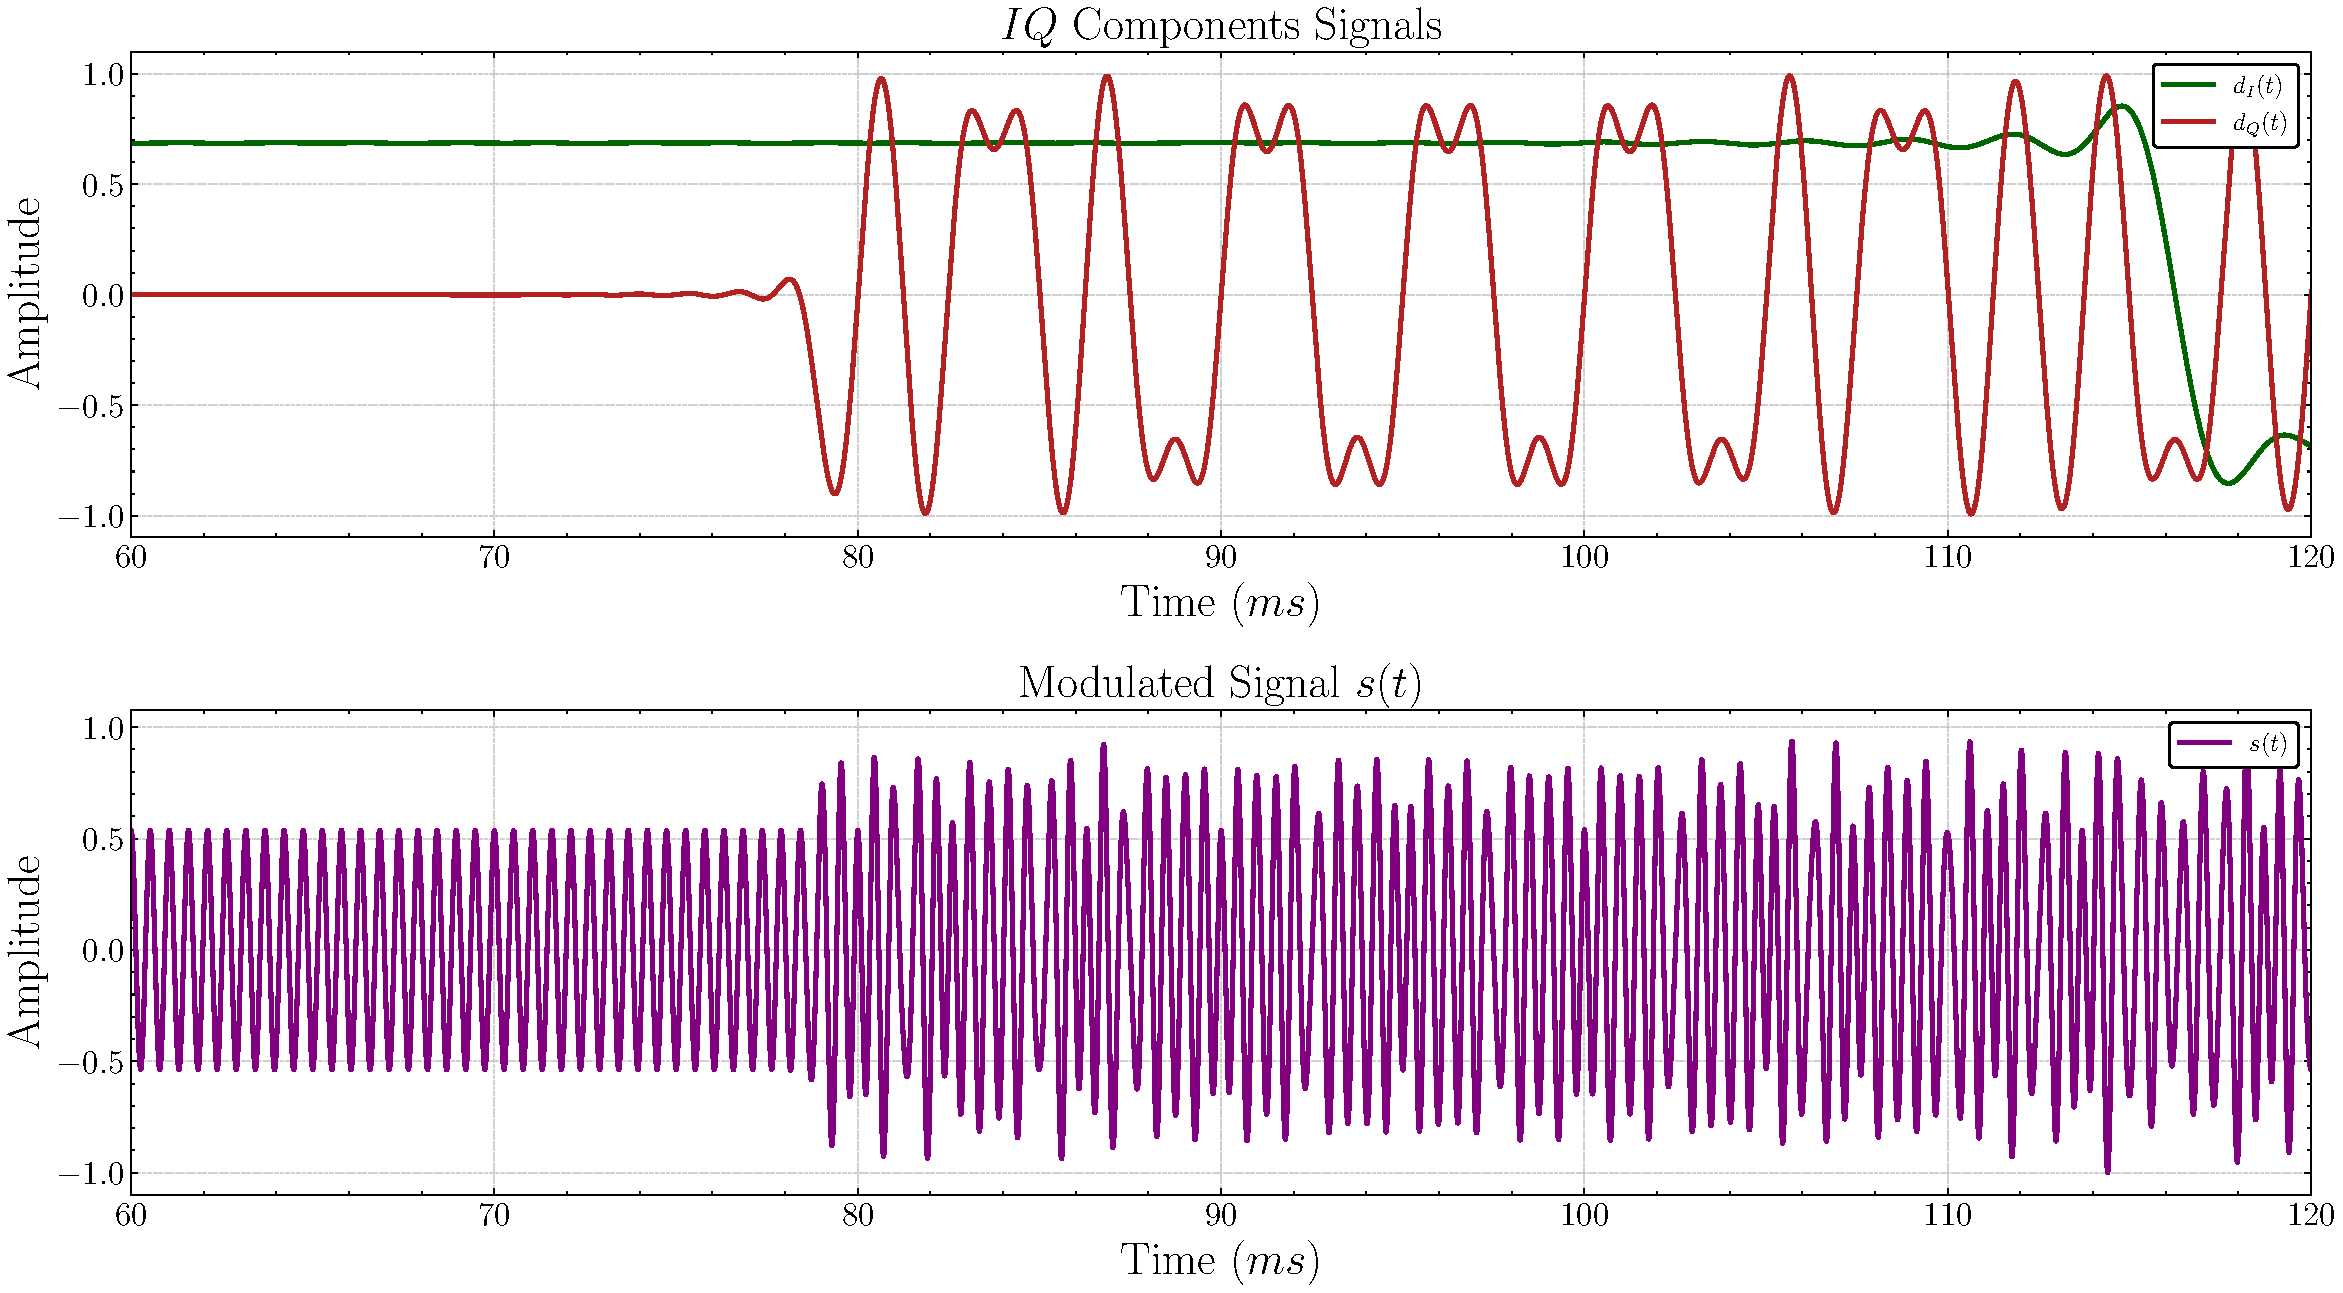
\includegraphics[width=\linewidth]{assets/cap3/transmitter_modulator_time.pdf}
\end{figure}

A partir do sinal modulado \gls{st}, é possível observar a constelação do sinal \gls{QPSK}, isto é o comportamento do sinal \gls{st} no \gls{iqplane}, que idealmente para o \gls{QPSK} é composto por quatro pontos distintos, cada um representando uma combinação única dos bits transmitidos pelos canais \gls{cI} e \gls{cQ}. A constelação do sinal modulado \gls{st} é ilustrada na \autoref{fig:transmitter_modulator_constellation}, onde é possível observar a fase do sinal modulado e a constelação resultante no \gls{iqplane}.


\begin{figure}[H]
	\centering
	\caption{Fase e Constelação do sinal modulado $s(t)$}\label{fig:transmitter_modulator_constellation}
	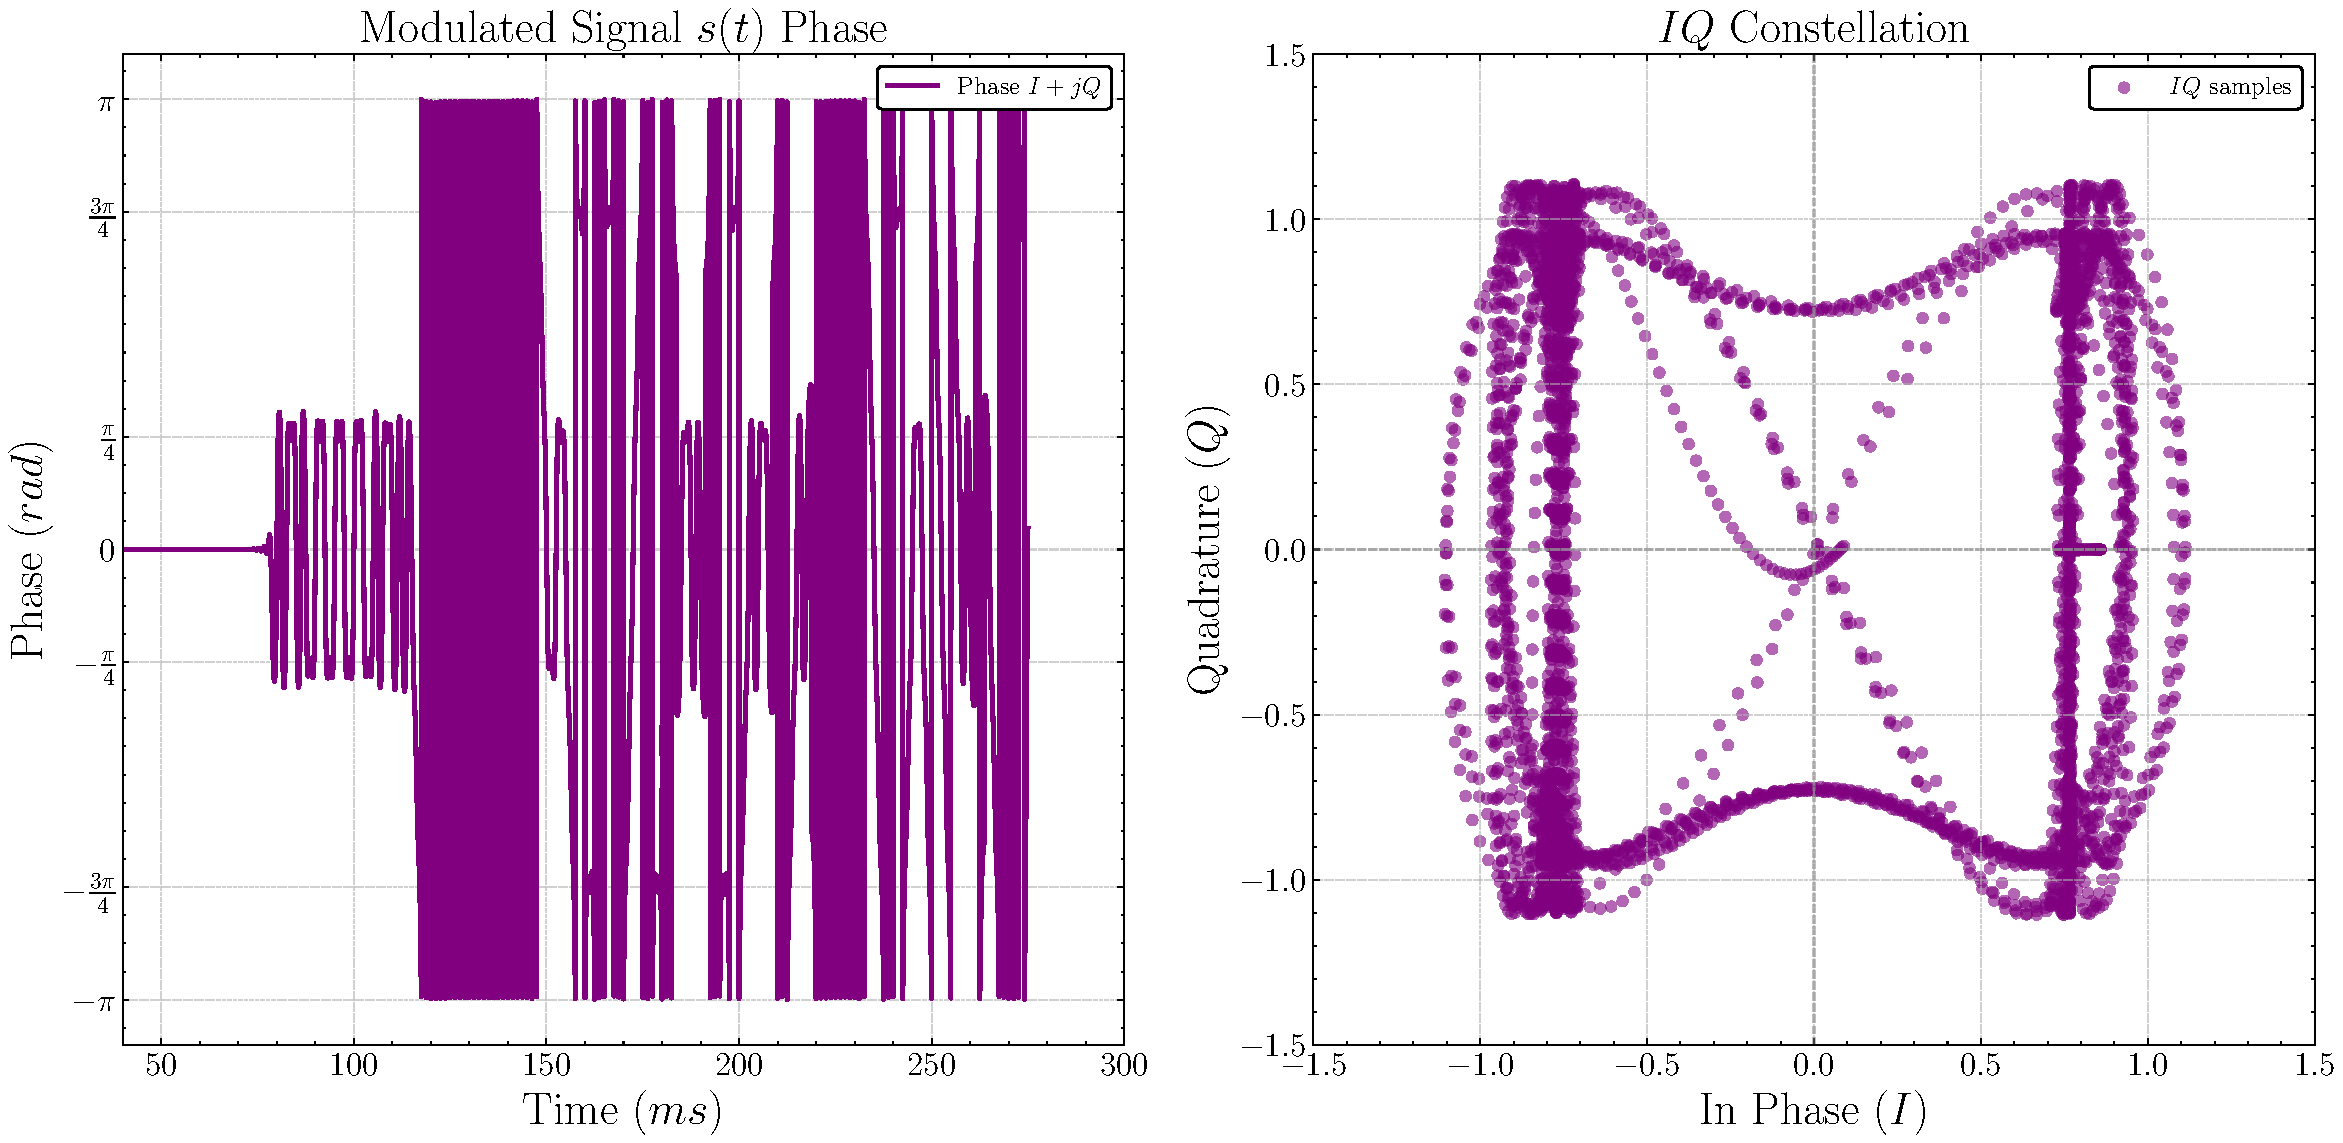
\includegraphics[width=\linewidth]{assets/cap3/transmitter_modulator_constellation.pdf}
\end{figure}


\subsubsection{Adição de portadora pura}

Ao se observar mais atentamente a \ref{fig:transmitter_modulator_time} e também \ref{fig:transmitter_formatter_time} pode-se notar que no inicio da transmissão, a componente \gls{dI} está com amplitude estável e proxima á $`1`$, enquanto que a componente \gls{dQ} está estável com amplitude igual a $`0`$, essa é configuração é proposital dentro do \gls{Pd} para que a sequência resultante modulada em banda passante tenha um periodo de fase estável, ou seja, uma portadora pura, antes do inicio da transmissão dos dados. O equacionamento para o período de portadora pura pode ser expresso como

\begin{equation}
    s(t) = 1(t) \cdot \cos(2\pi f_c t) - 0(t) \cdot \sin(2\pi f_c t) \mapsto s(t) = \cos(2\pi f_c t)
\end{equation}

\noindent Onde $1(t)$ é a componente \gls{dI} com valor constante $`1`$ e $0(t)$ é a componente \gls{dQ} com valor constante $`0`$. O período de portadora pura é fundamental para o receptor identificar a frequência da portadora \gls{fc} e realizar a detecção do sinal corretamente, conforme detalhado na seção \ref{sec:detector}. A duração do período de portadora pura é definida pelo parâmetro \gls{Pd}, que no padrão \gls{ARGOS-III} é aproximadamente $0.082$ segundos.

Com o sinal modulado em banda passante \gls{st} conforme definido acima, podemos também verificar a presença da portadora pura nos primeiros instantes da transmissão, isto é ilustrado na figura \ref{fig:transmitter_modulator_portadora} apresentada abaixo.

\begin{figure}[H]
	\centering
	\caption{Comparação de portadora pura e sinal modulado}\label{fig:transmitter_modulator_portadora}
	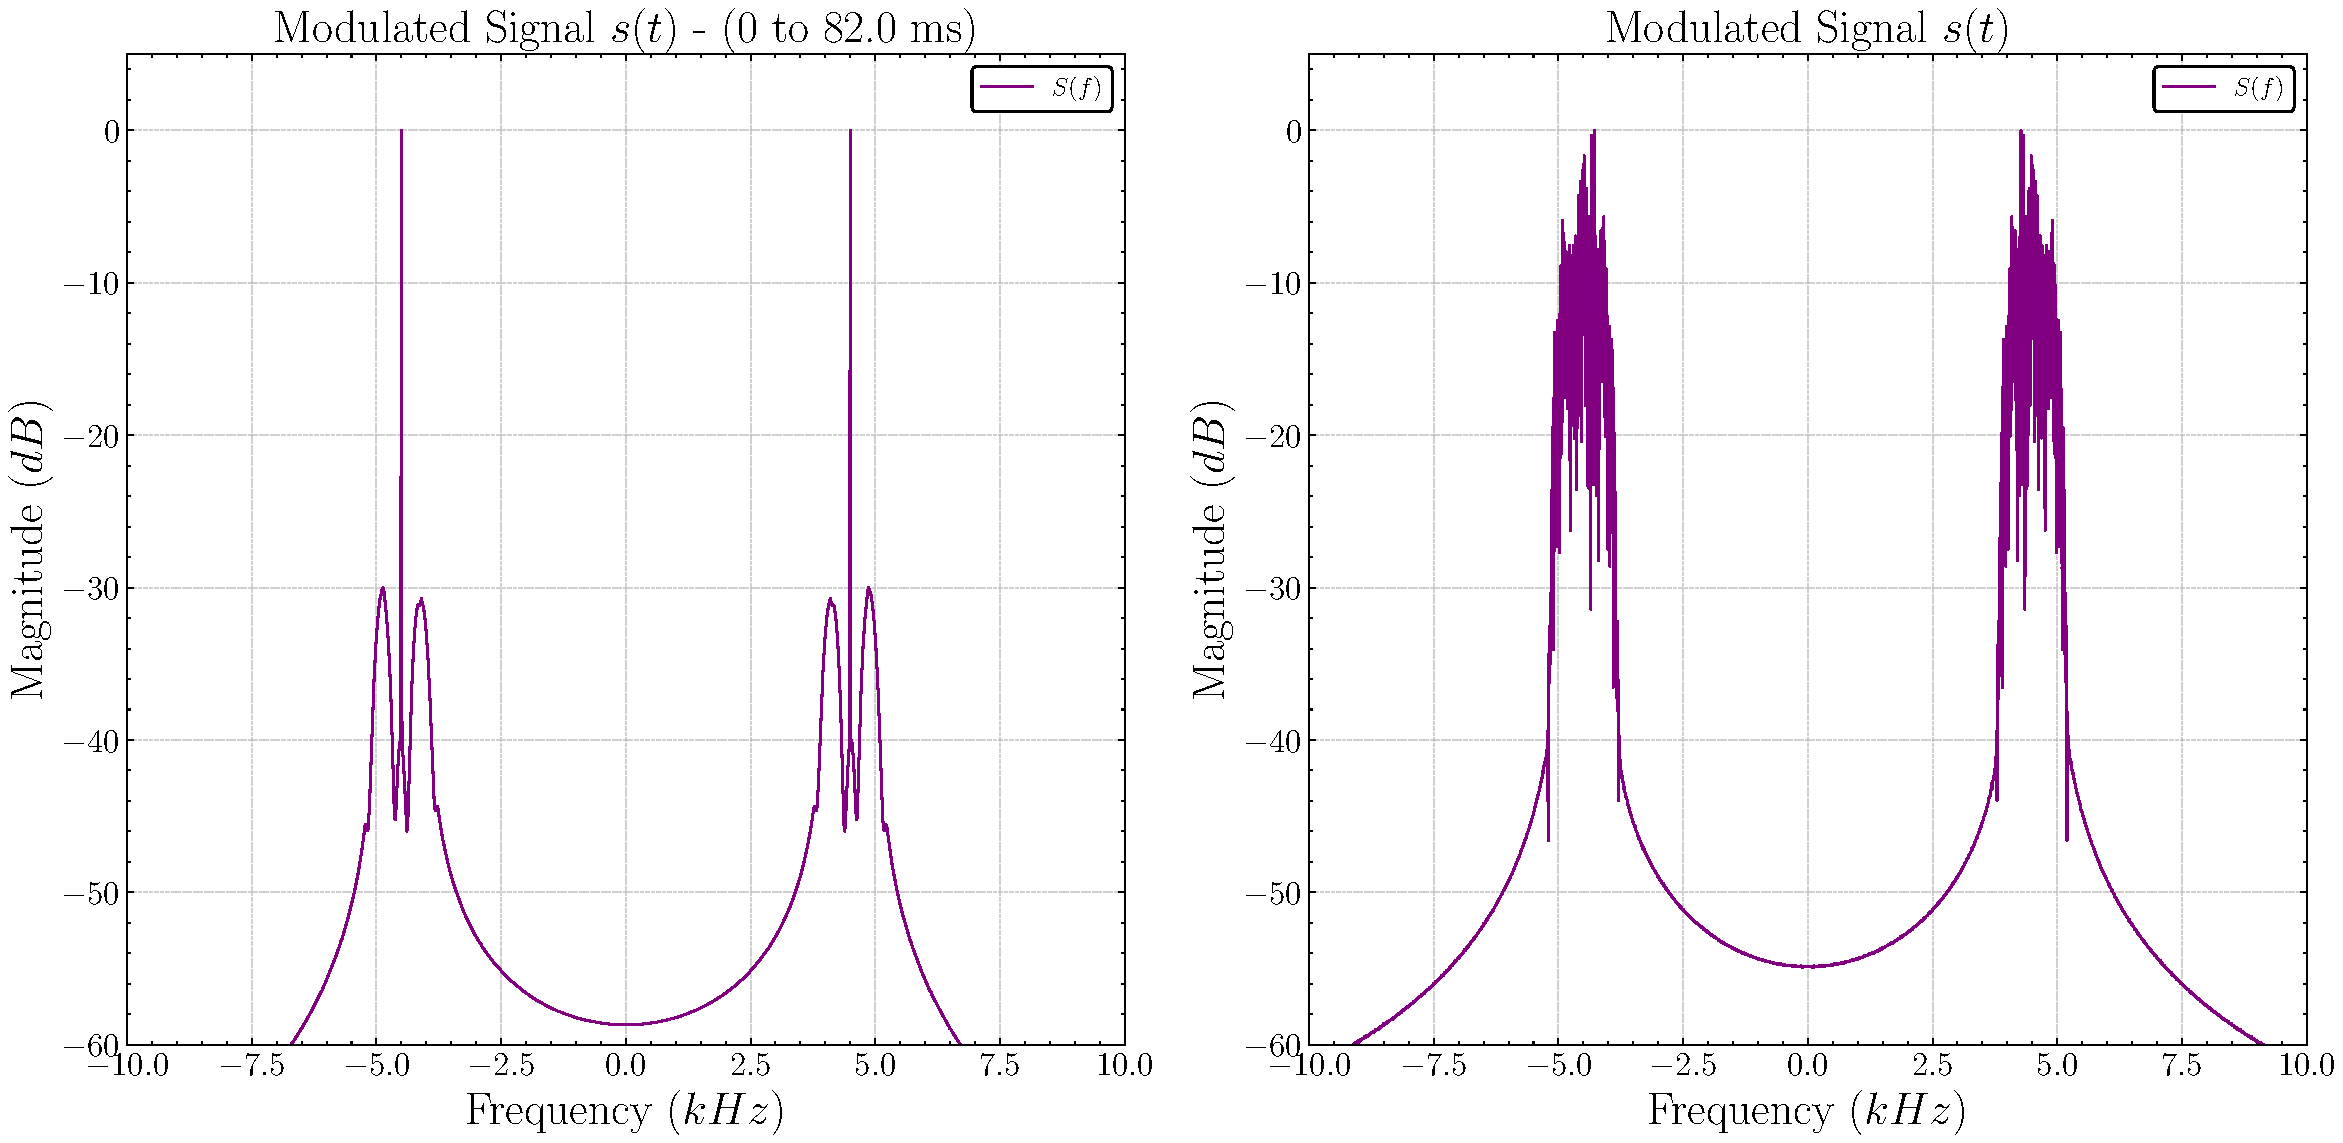
\includegraphics[width=\linewidth]{assets/cap3/transmitter_modulator_portadora.pdf}
\end{figure}

\section{CANAL E ADIÇÃO DE RUÍDO}\label{sec:canal}



\begin{figure}[H]
	\centering
	\caption{Diagrama de blocos do canal}\label{fig:channel_diagram}
	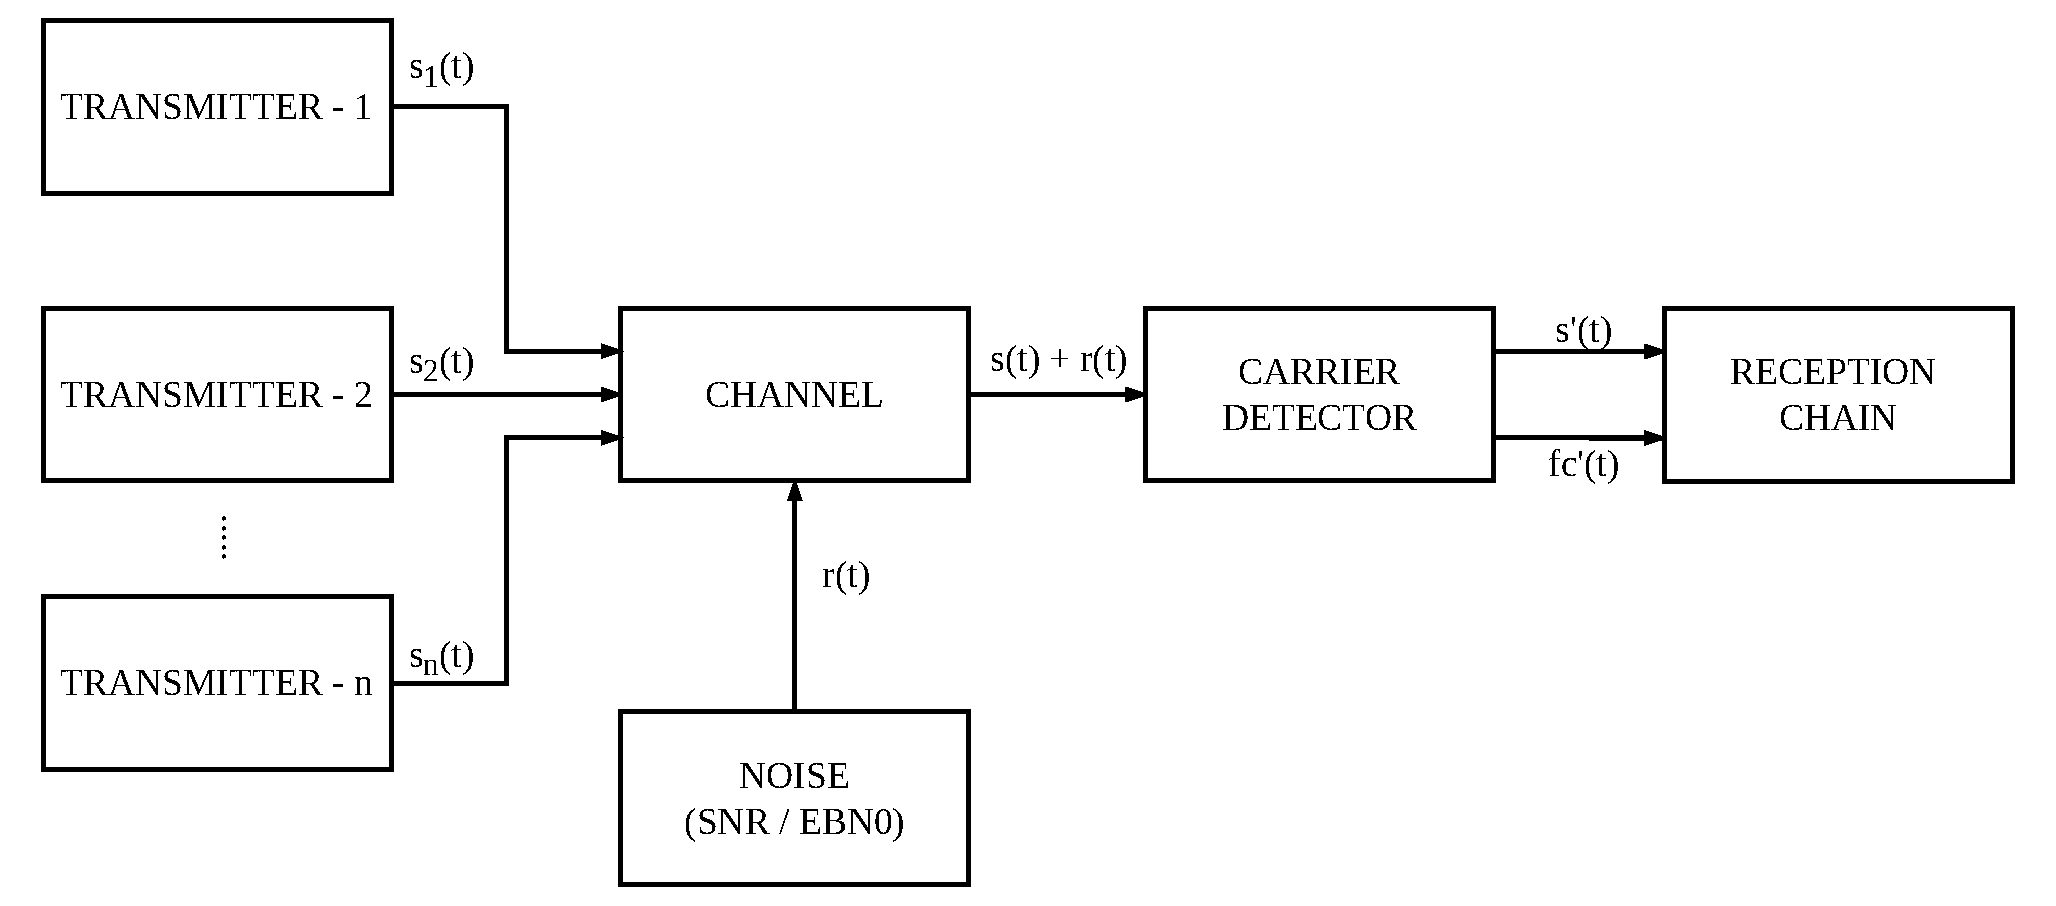
\includegraphics[width=\linewidth]{assets/diagrams/channel.pdf}
\end{figure}

\subsection{Modelo de canal}\label{sec:modelo_canal}

\begin{figure}[H]
	\centering
	\caption{Adição de multiplas transmissões no canal}\label{fig:channel_time}
	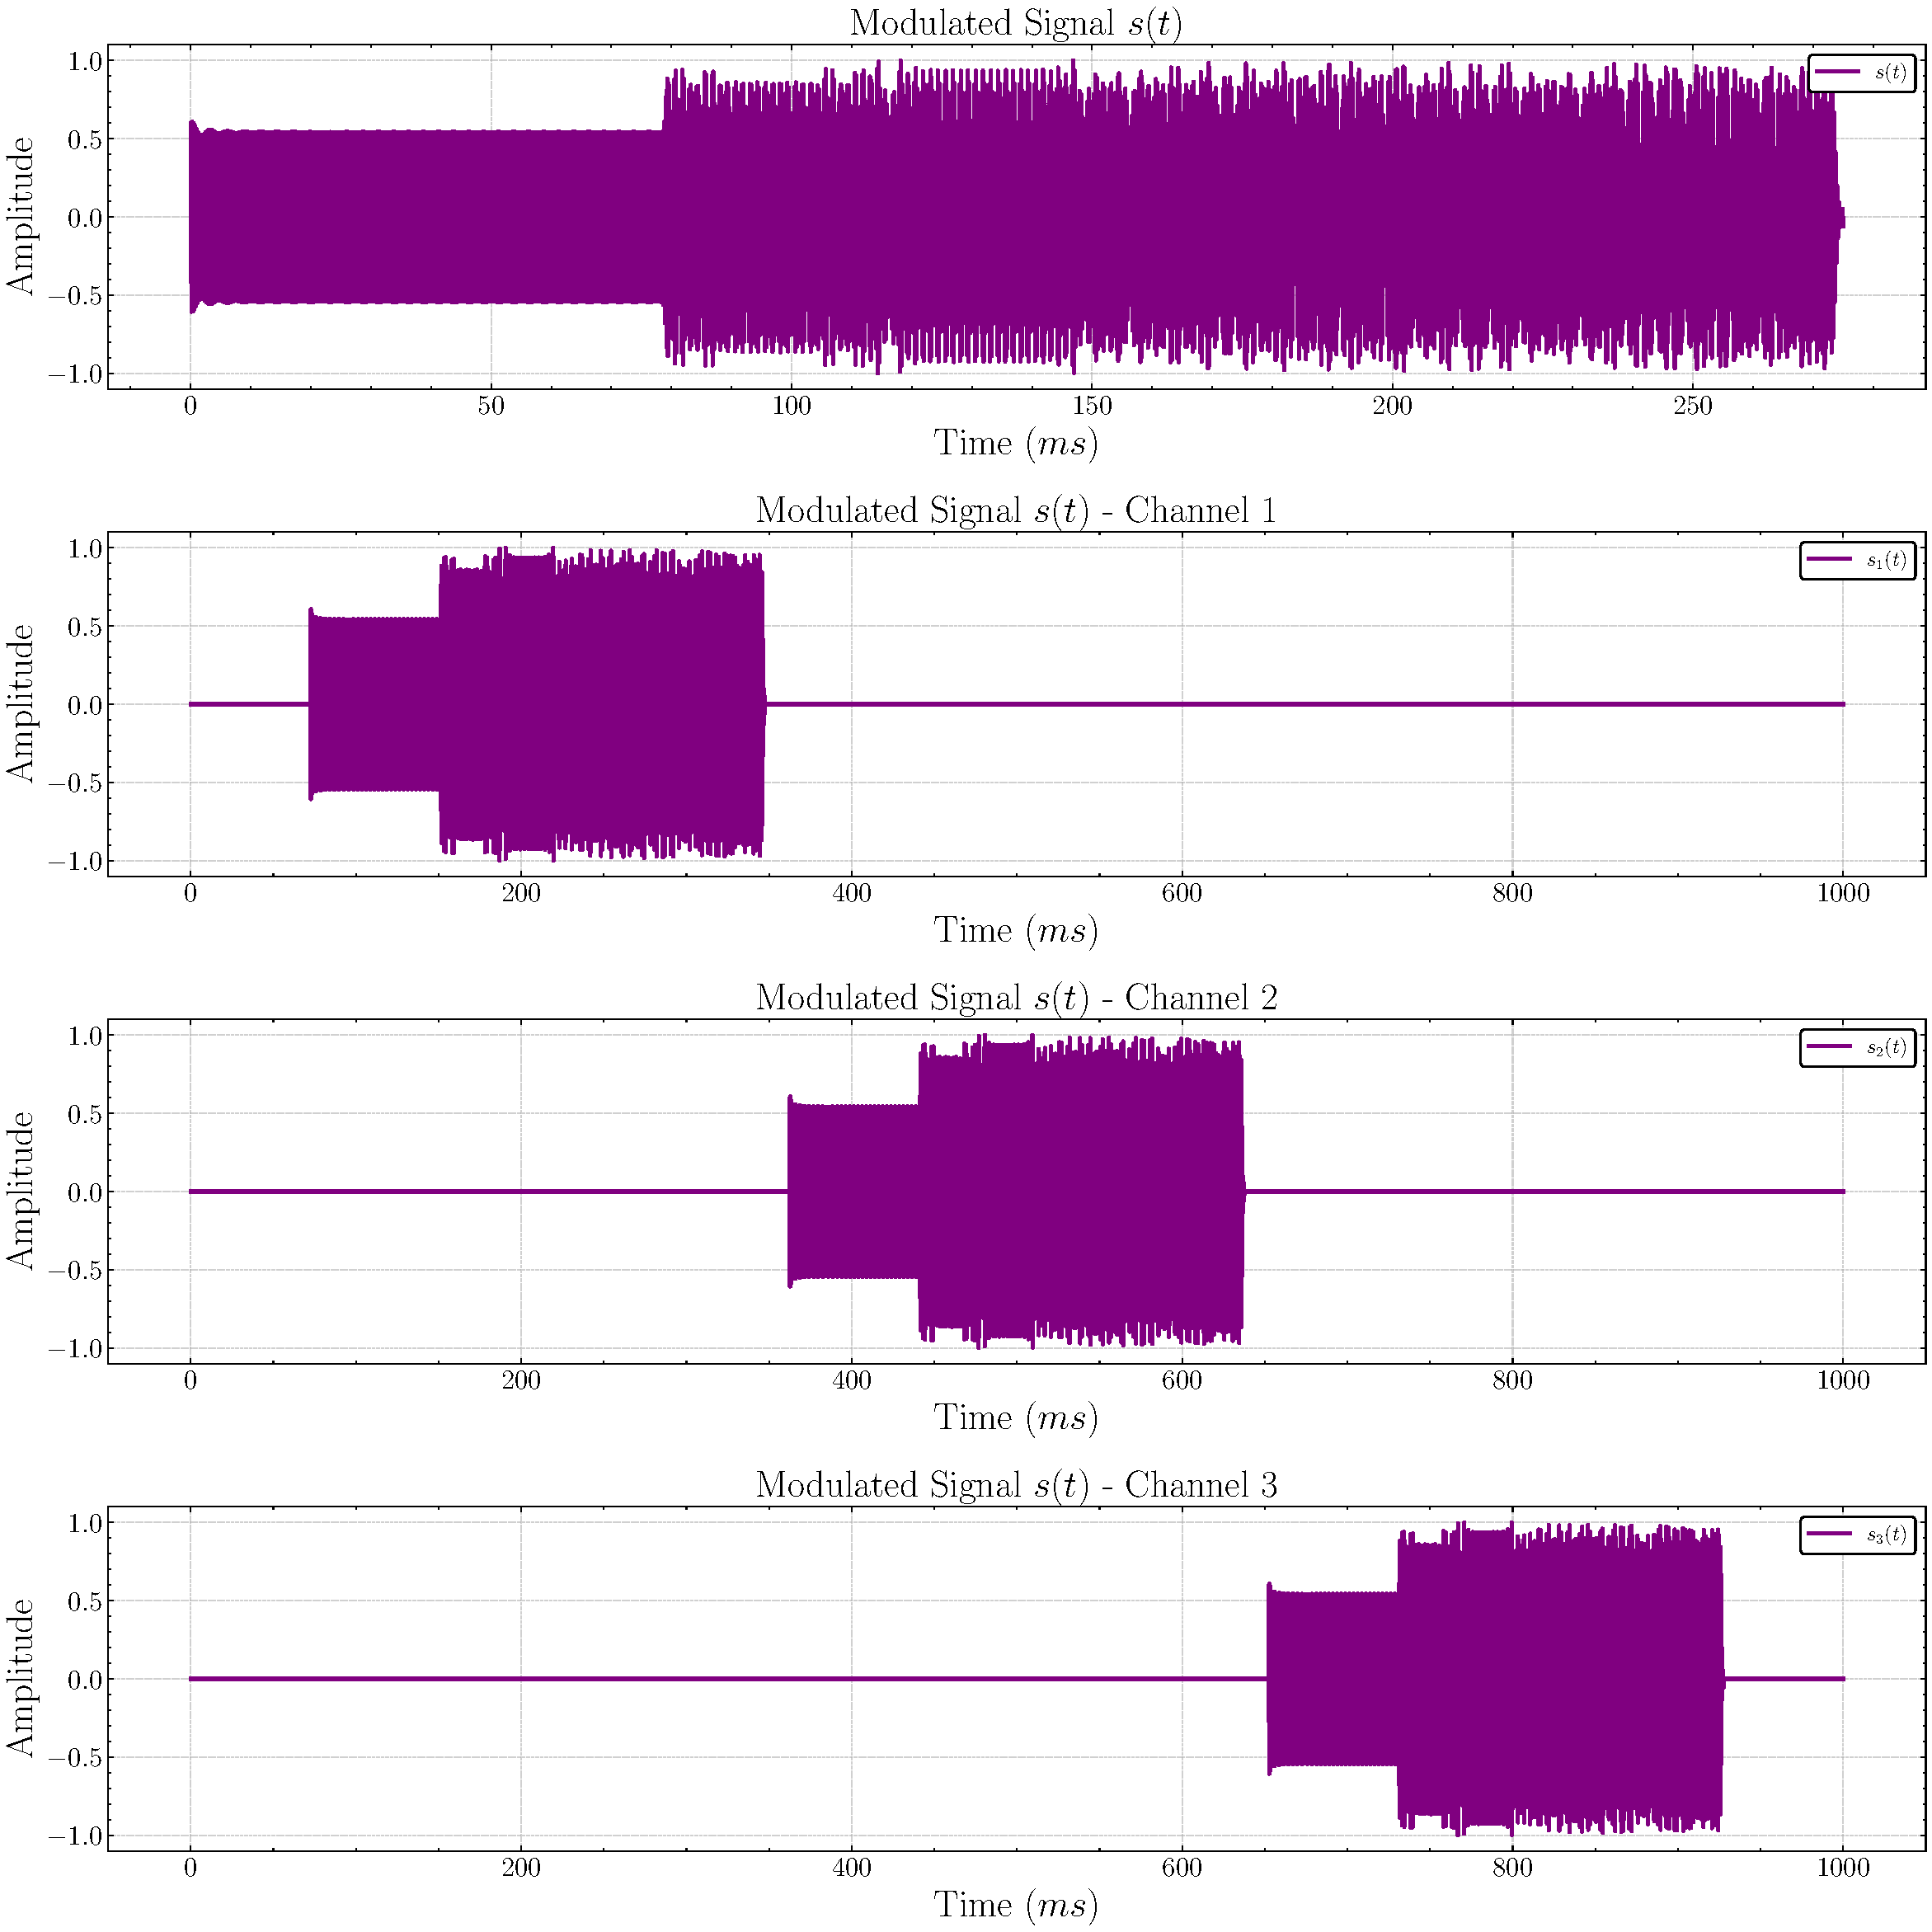
\includegraphics[width=\linewidth]{assets/cap3/example_channel_time_subchannels.pdf}
\end{figure}

\subsection{Geração de ruído AWGN}\label{sec:geracao_ruido}

\begin{figure}[H]
	\centering
	\caption{Adição de ruído ao canal}\label{fig:add_noise_time}
	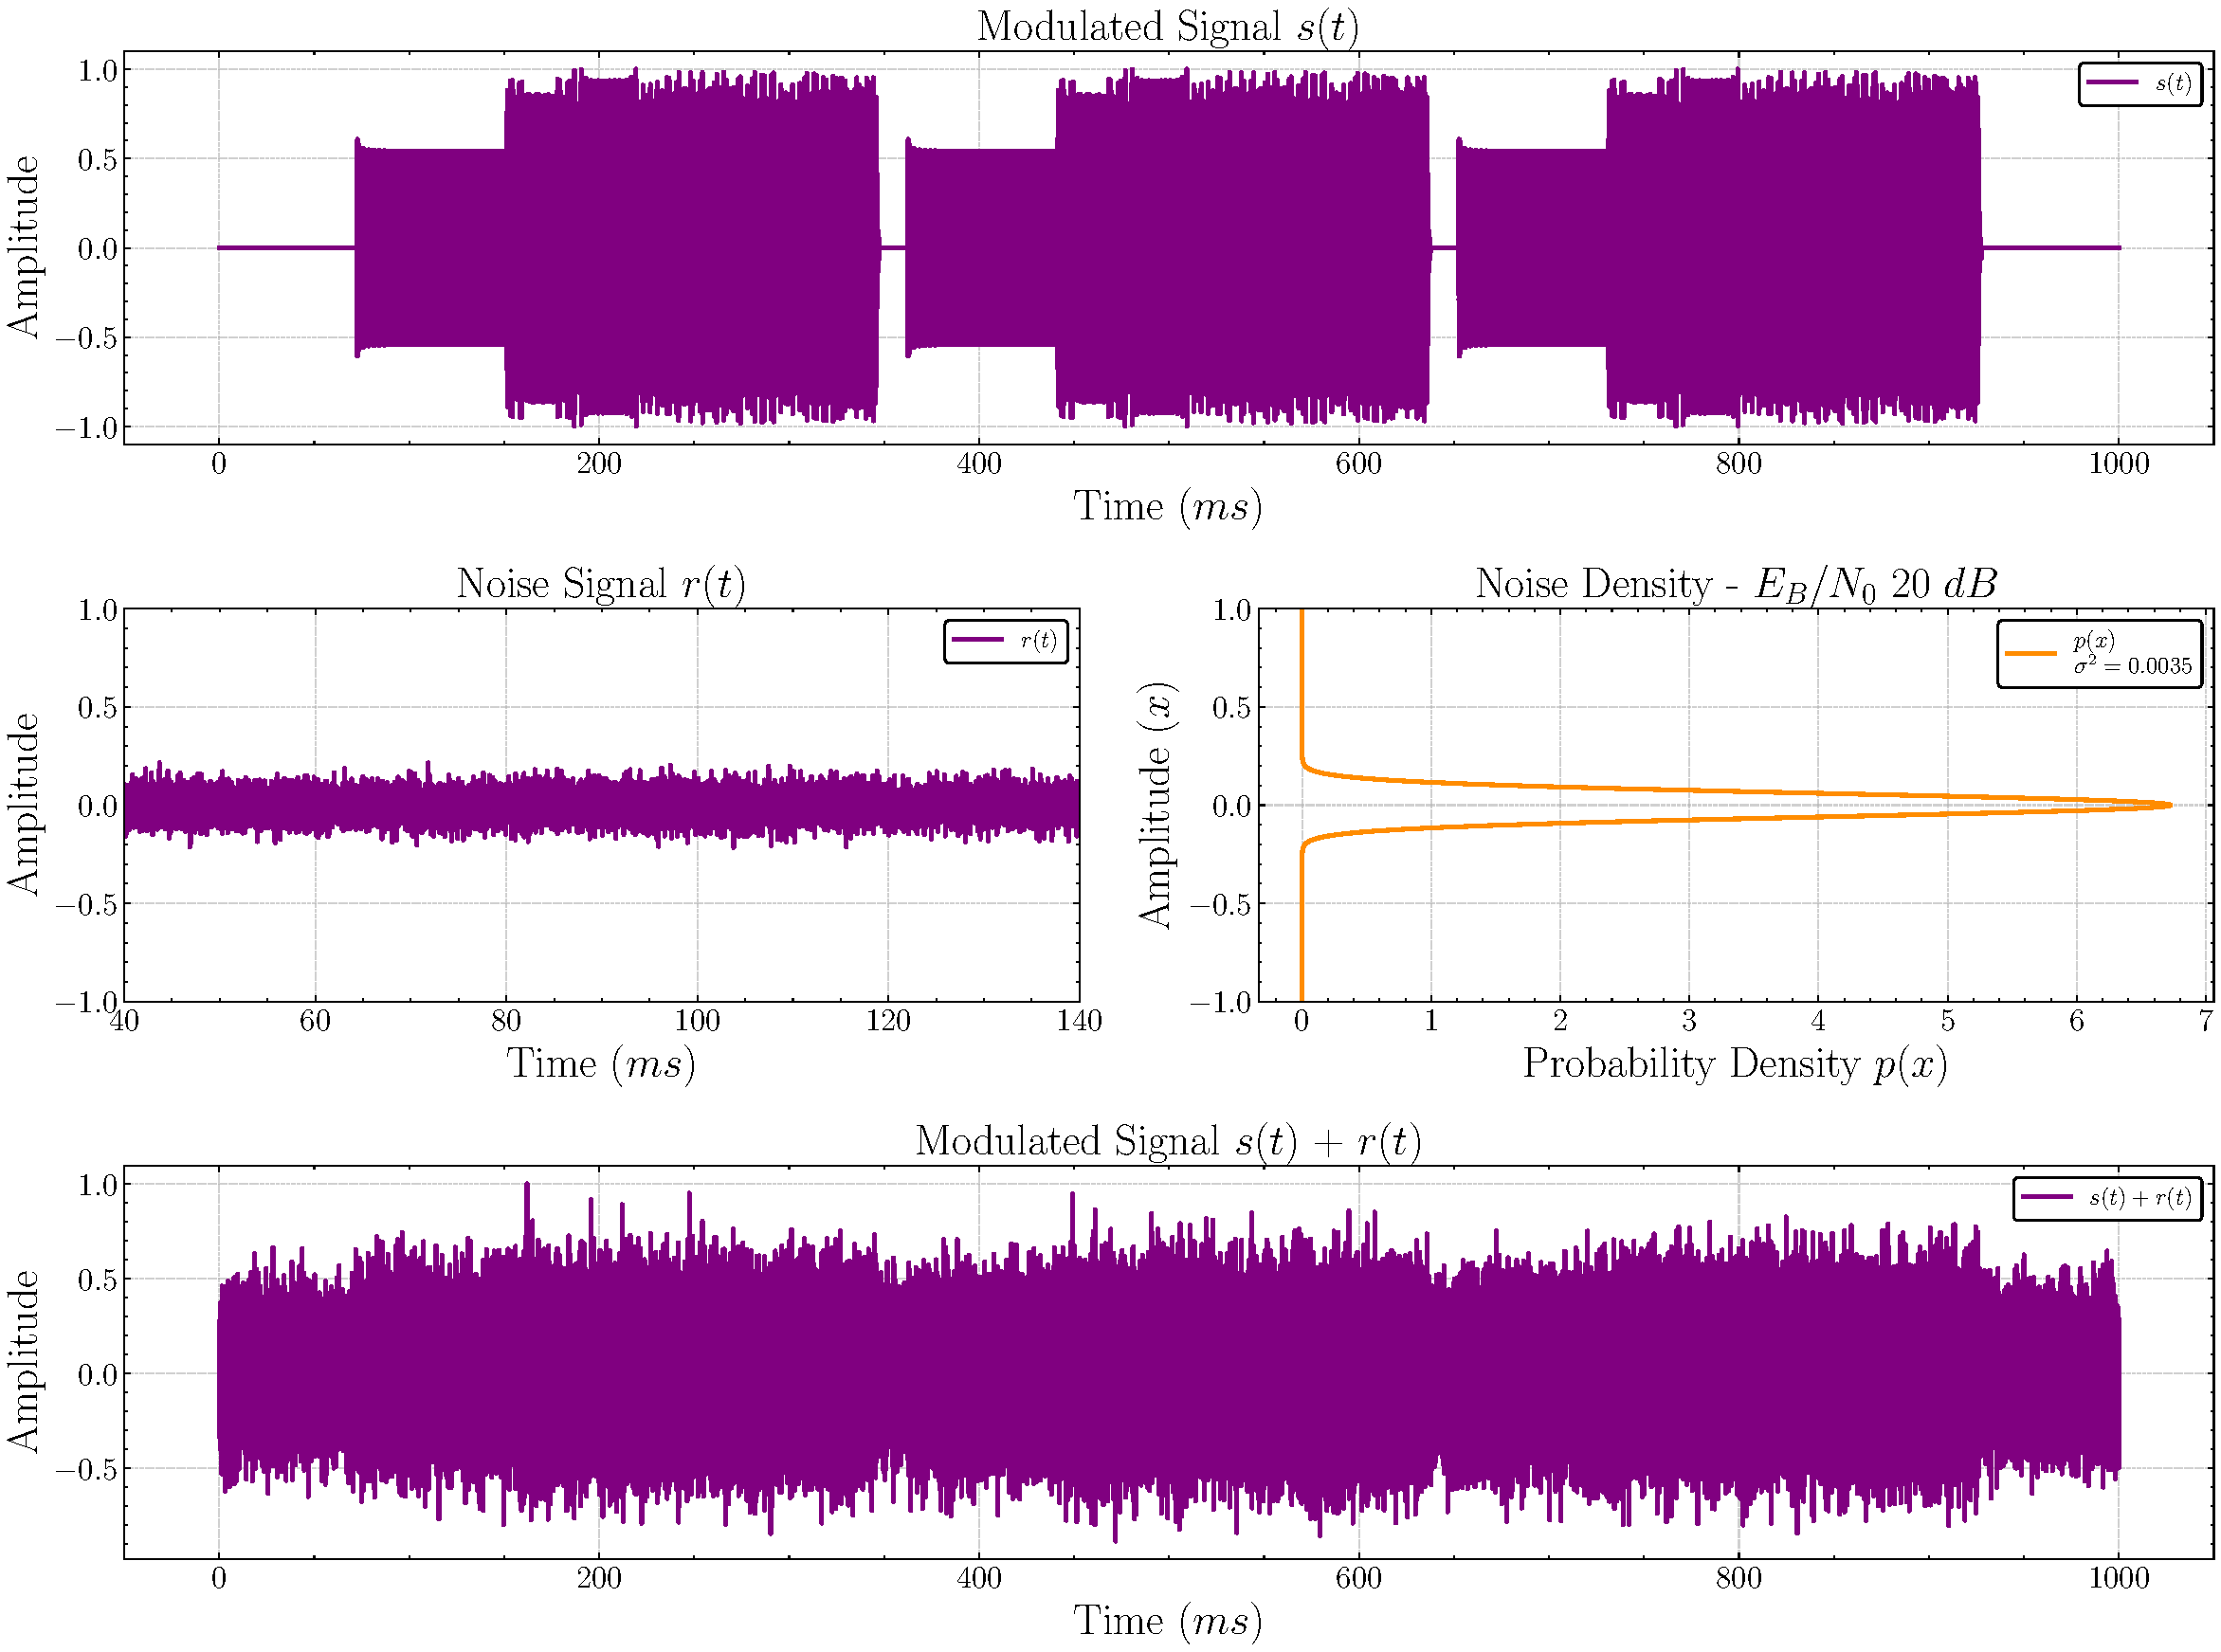
\includegraphics[width=\linewidth]{assets/cap3/example_channel_time_channel.pdf}
\end{figure}

\section{DETECÇÃO DE PORTADORA}\label{sec:detector}

\begin{figure}[H]
	\centering
	\caption{Diagrama de blocos da detecção de portadora}\label{fig:detector_diagram}
	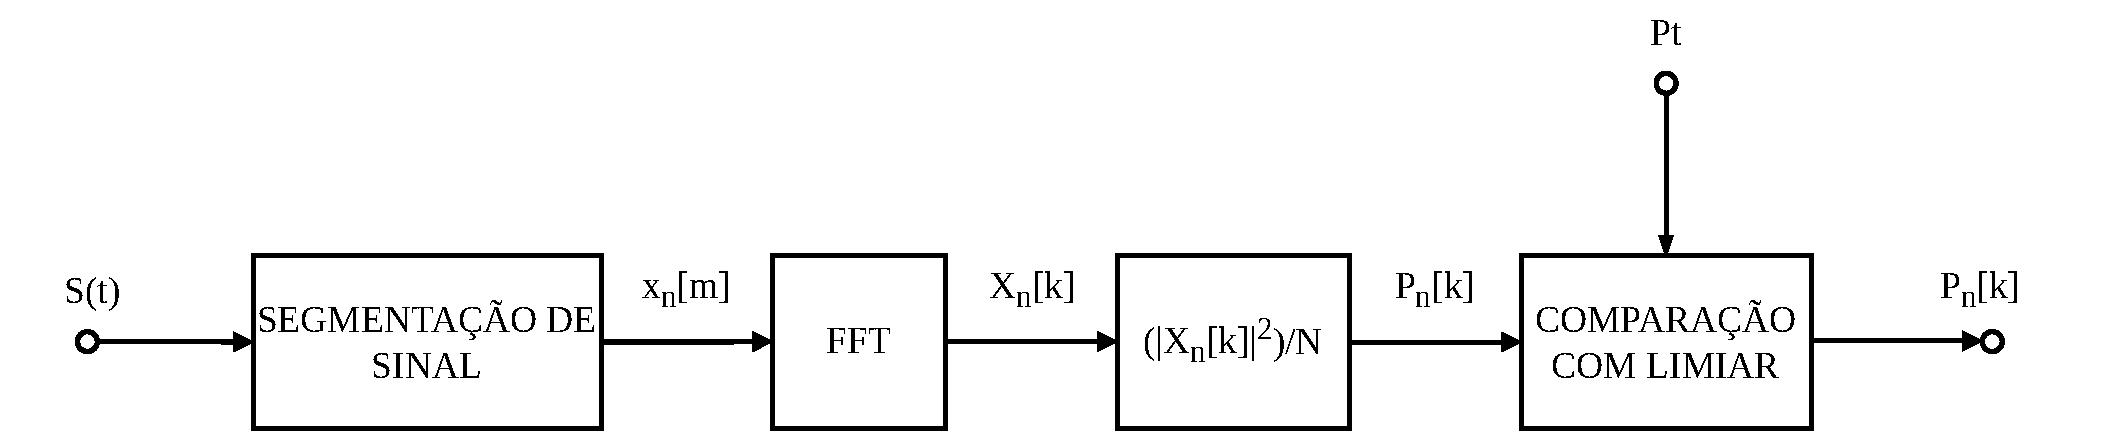
\includegraphics[width=\linewidth]{assets/diagrams/detector.pdf}
\end{figure}

\subsection{Segmentação do sinal recebido}\label{sec:segmentacao}

\begin{figure}[H]
	\centering
	\caption{Diagrama de waterfall do canal}\label{fig:waterfall}
	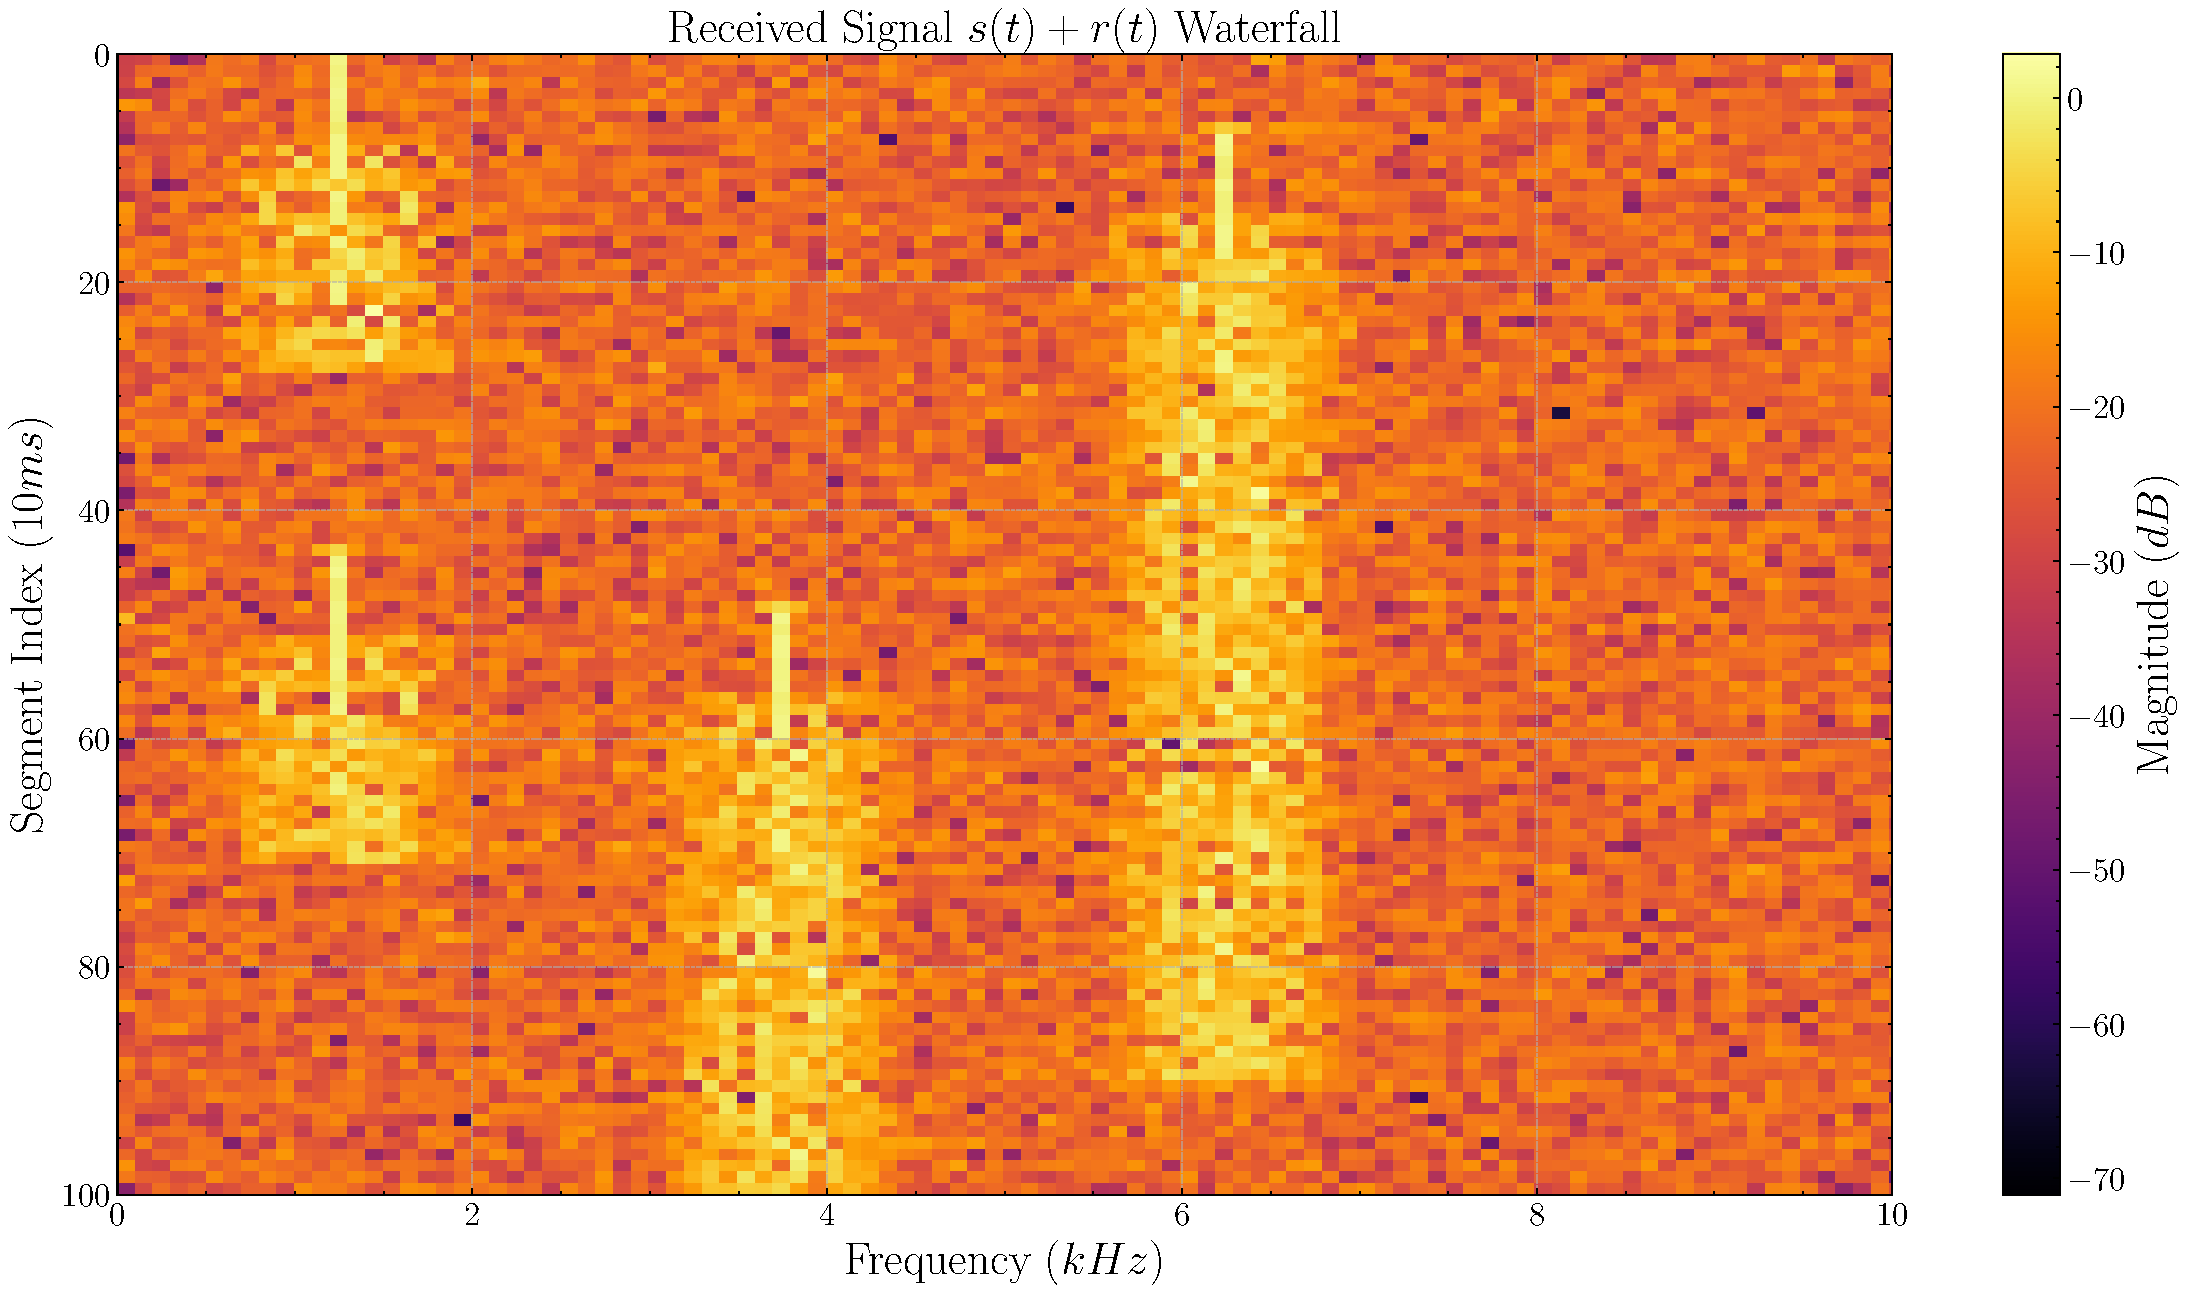
\includegraphics[width=\linewidth]{assets/cap3/example_detector_waterfall.pdf}
\end{figure}


\subsection{Detecção de componentes no espectro}\label{sec:comparacao_potencia}

\begin{figure}[H]
	\centering
	\caption{Detecção de componentes no espectro com base em $P_t$}\label{fig:freq_detection}
	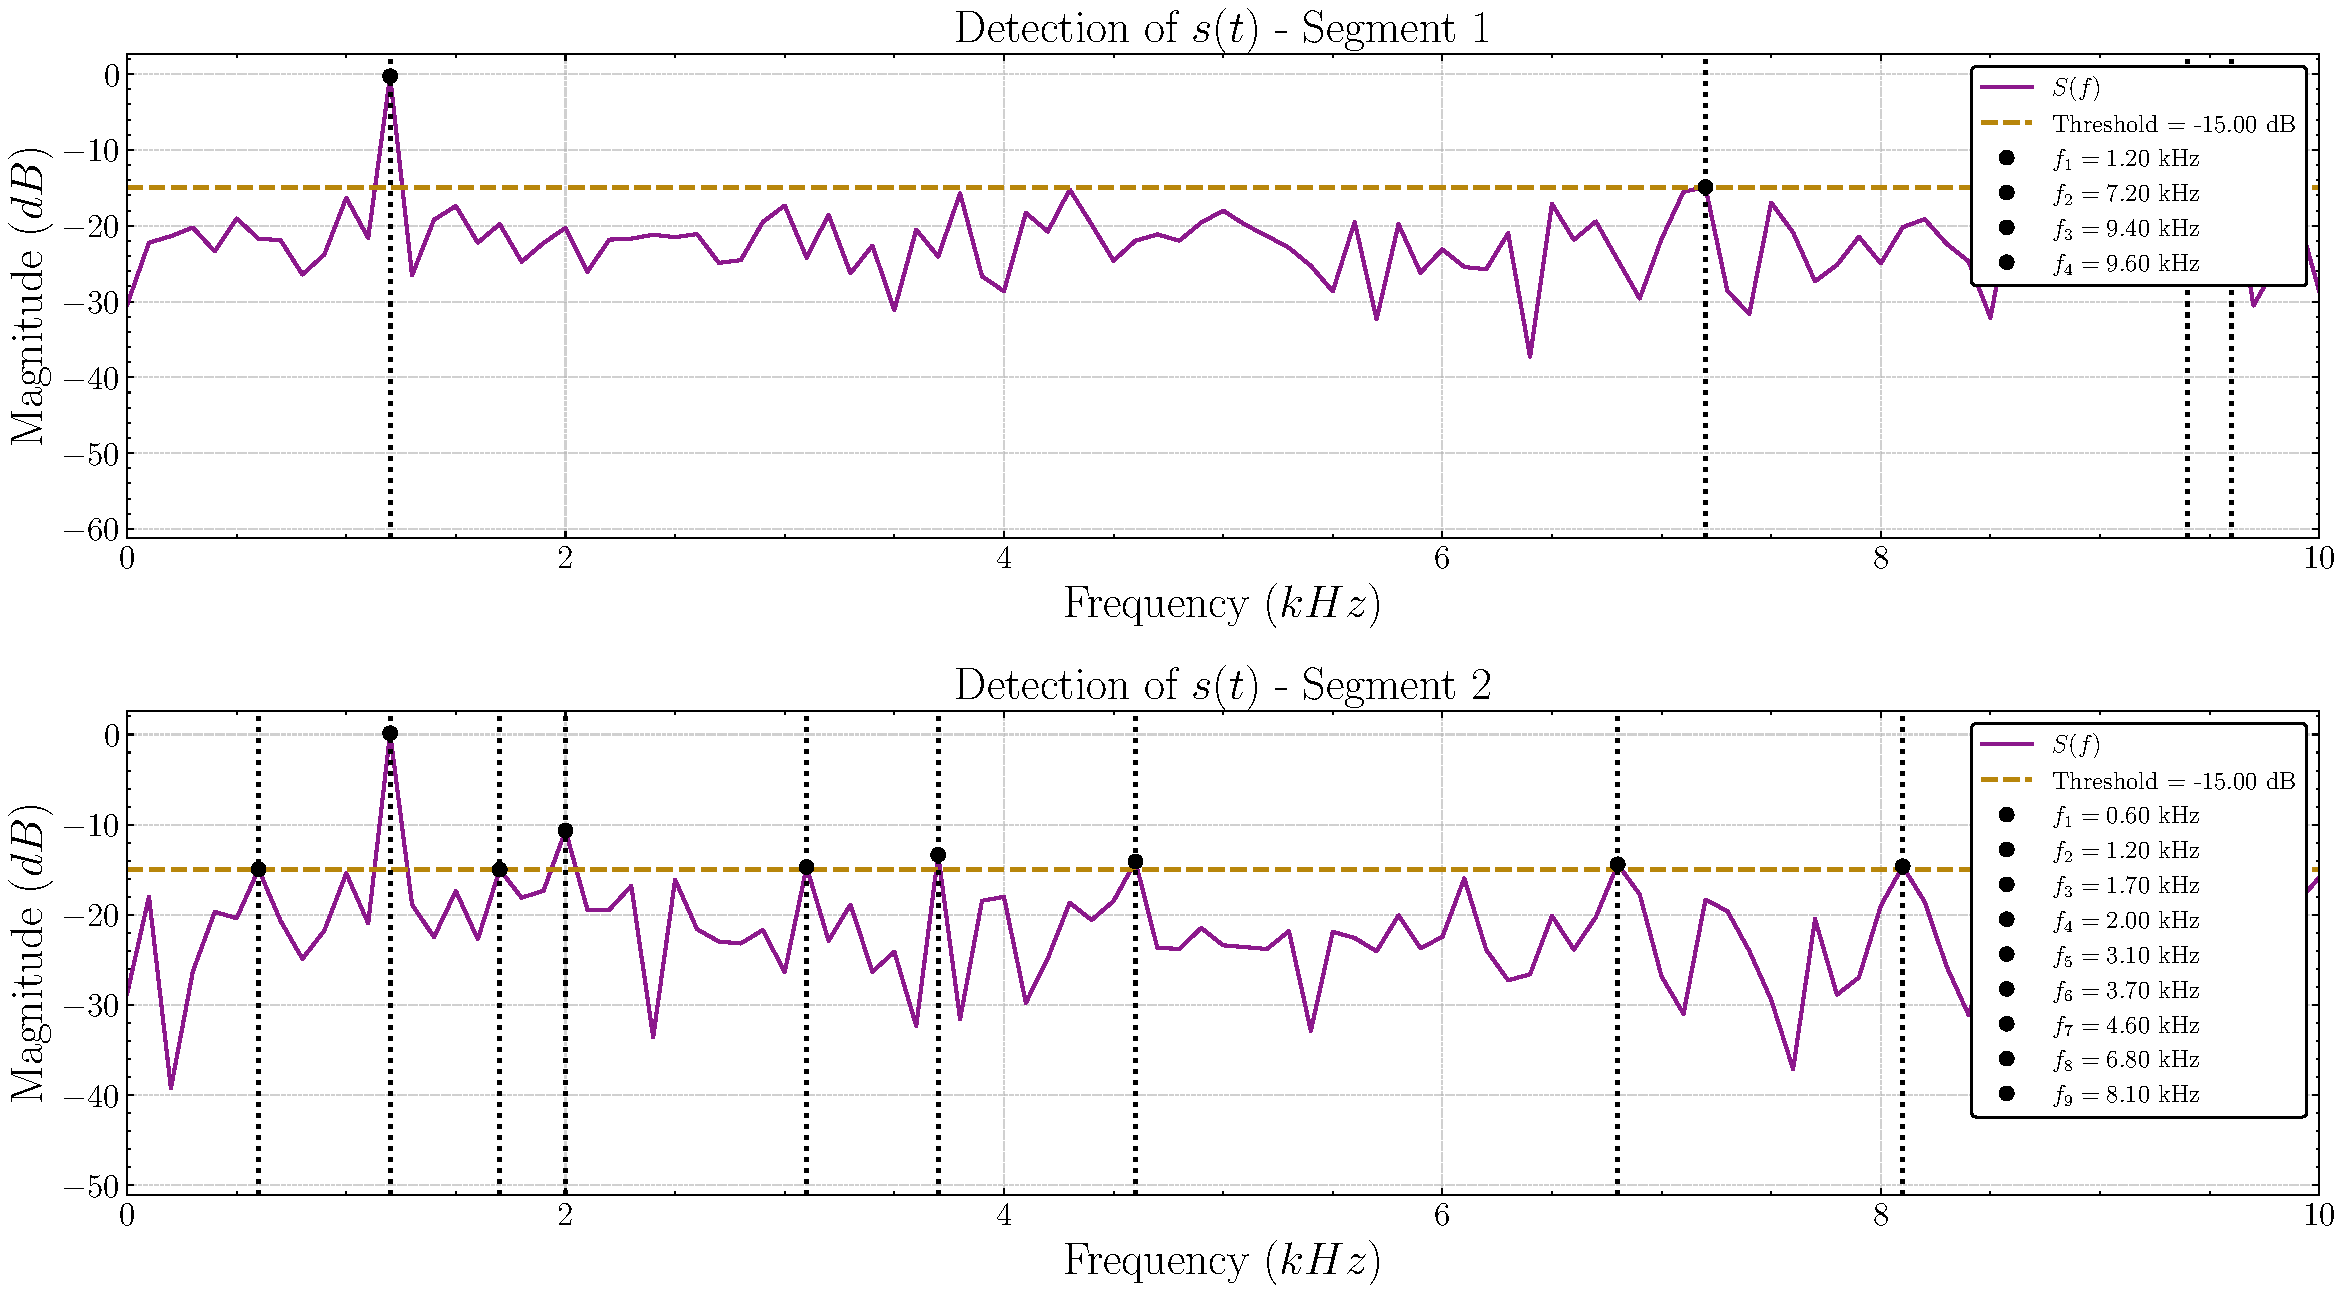
\includegraphics[width=\linewidth]{assets/cap3/example_detector_freq.pdf}
\end{figure}

\begin{figure}[H]
	\centering
	\caption{Diagrama de waterfall de detecção do canal}\label{fig:waterfall_detection}
	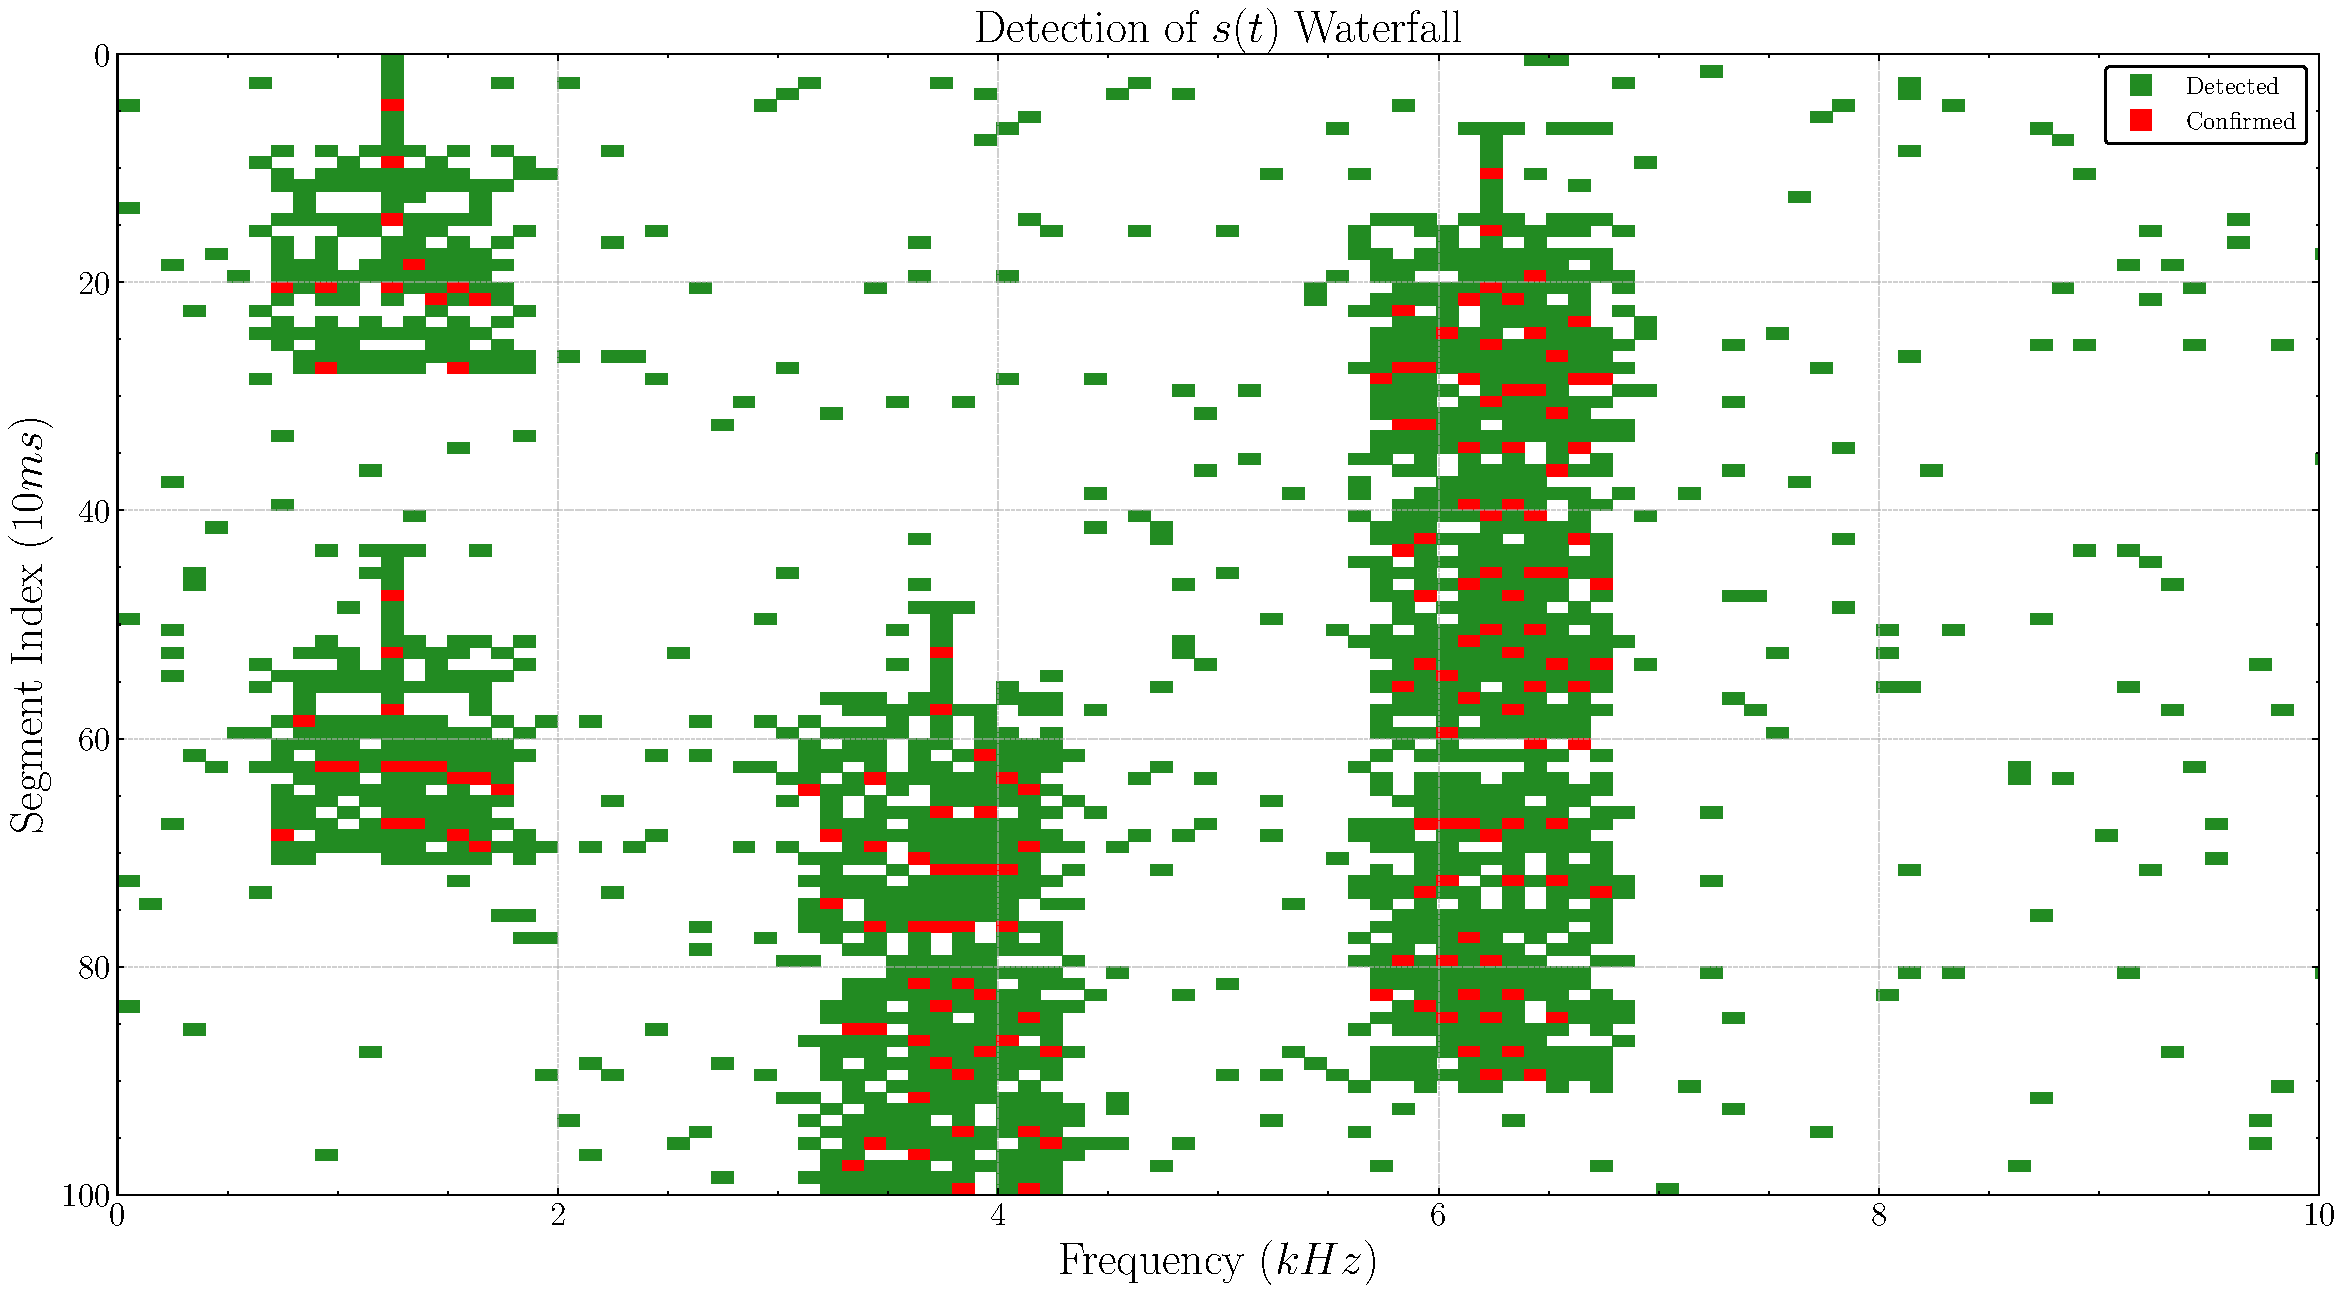
\includegraphics[width=\linewidth]{assets/cap3/example_detector_waterfall_detection.pdf}
\end{figure}


\subsection{Decisão de componentes detectadas}\label{sec:decisao}

\begin{figure}[H]
	\centering
	\caption{Diagrama de waterfall de decisão do canal}\label{fig:waterfall_decision}
	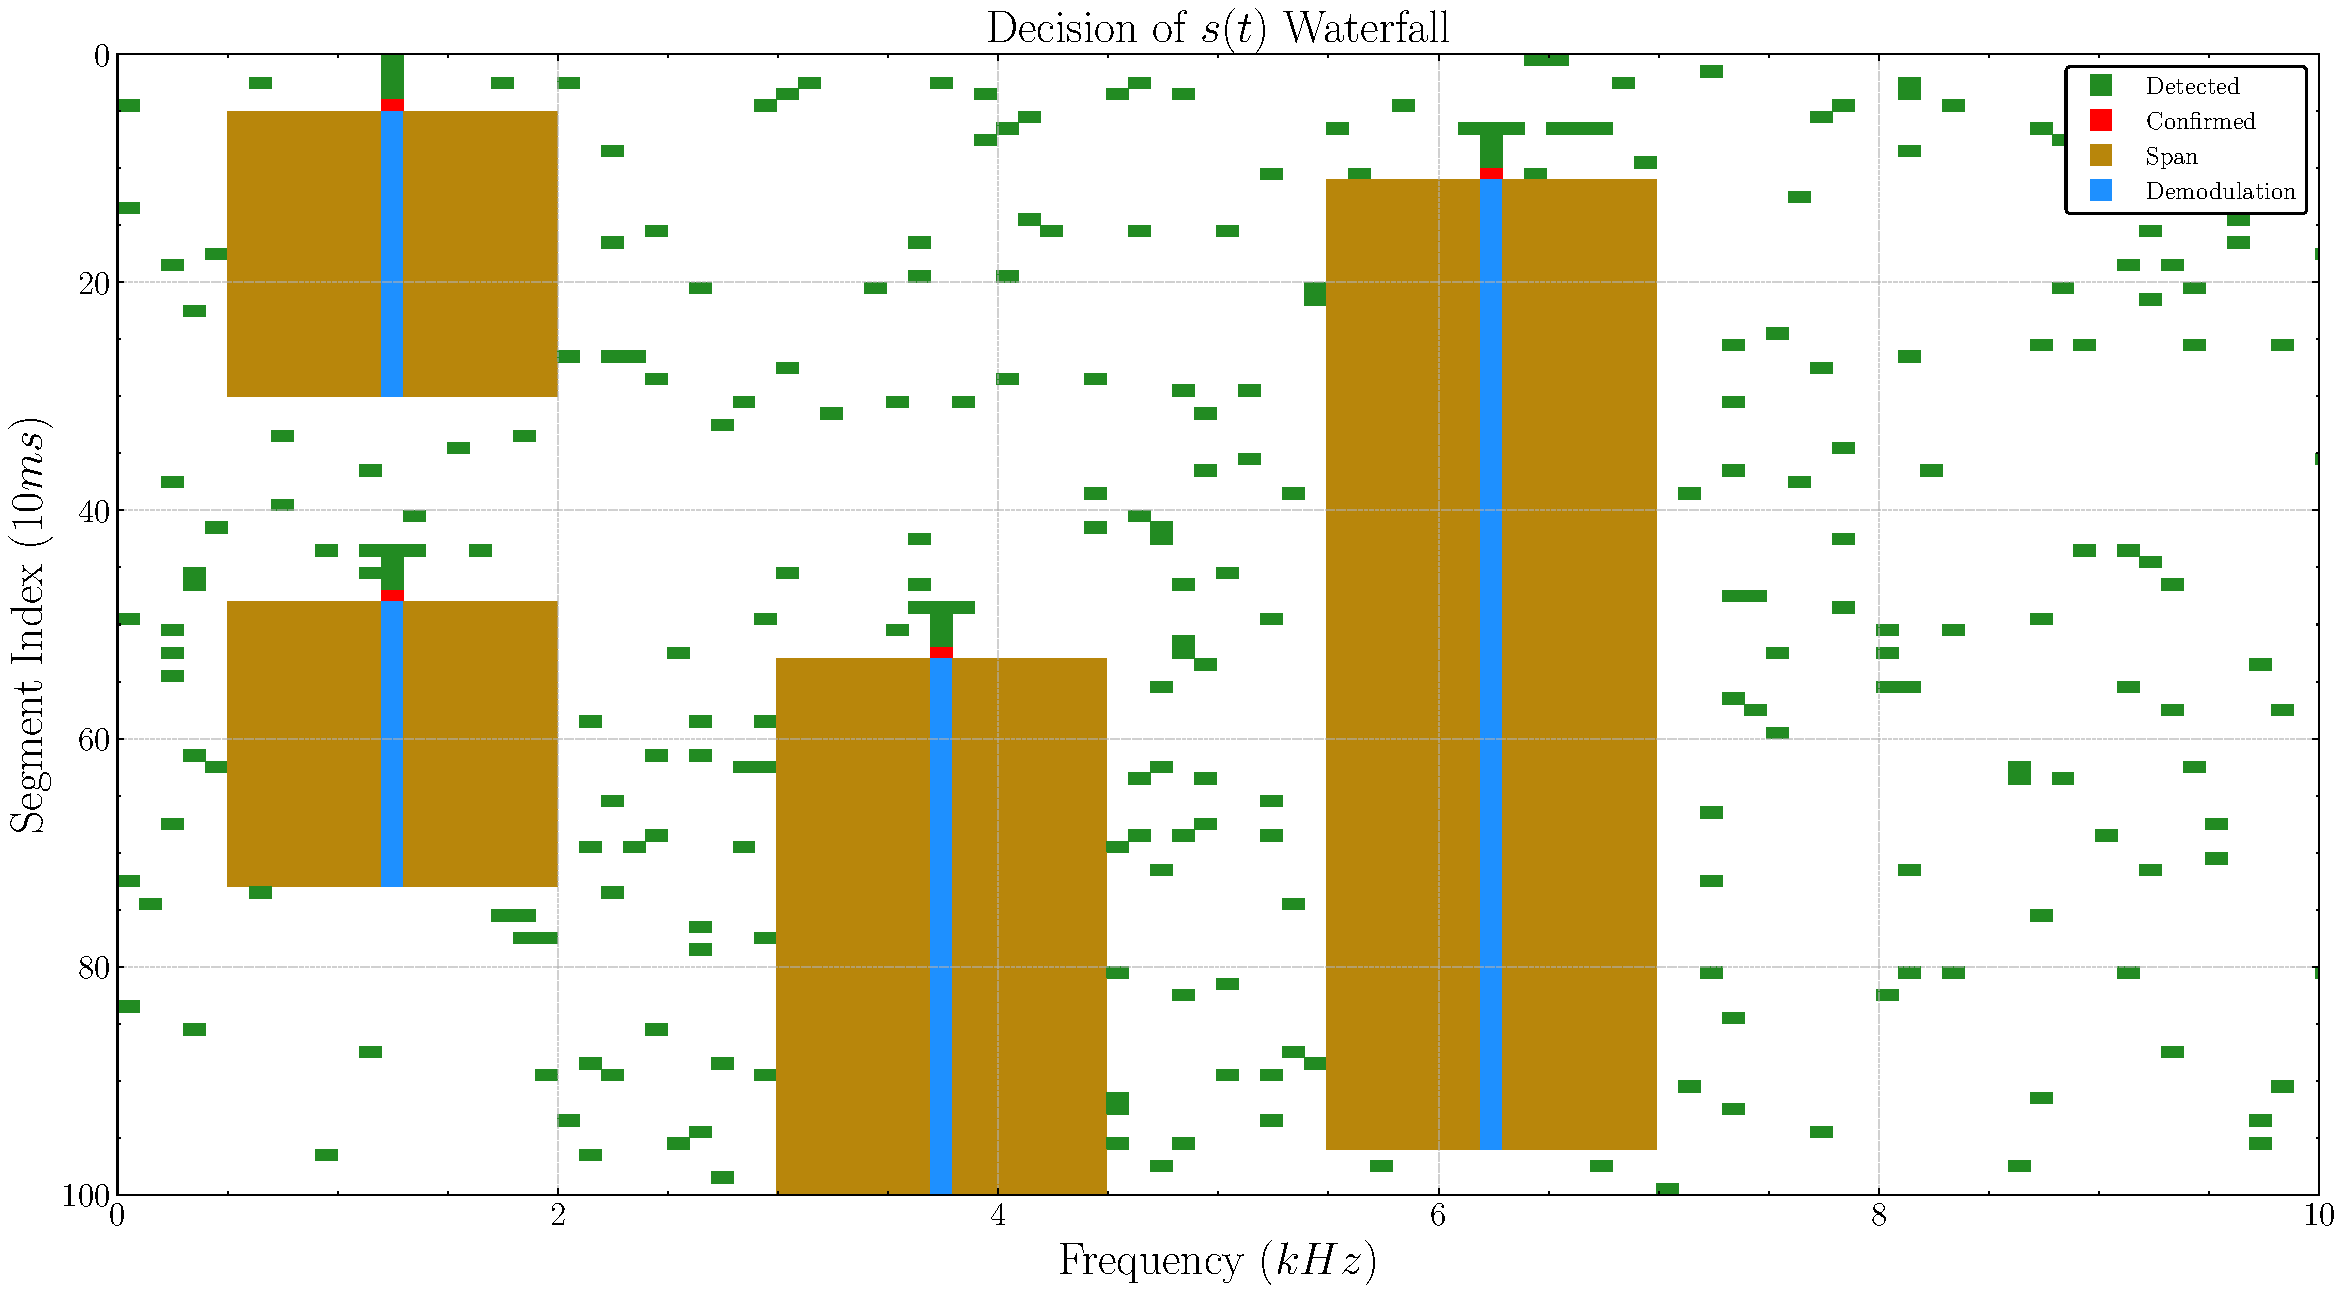
\includegraphics[width=\linewidth]{assets/cap3/example_detector_waterfall_decision.pdf}
\end{figure}

\subsection{Segmentação do sinal recebido para recepção}\label{sec:segmentacao_recepcao}

\section{CADEIA DE RECEPÇÃO}\label{sec:recepcao}    

\subsection{Demodulação banda base}\label{sec:demodulacao}

\begin{figure}[H]
	\centering
	\caption{Demodulação banda base dos canais $I$ e $Q$}\label{fig:receiver_demodulator}
	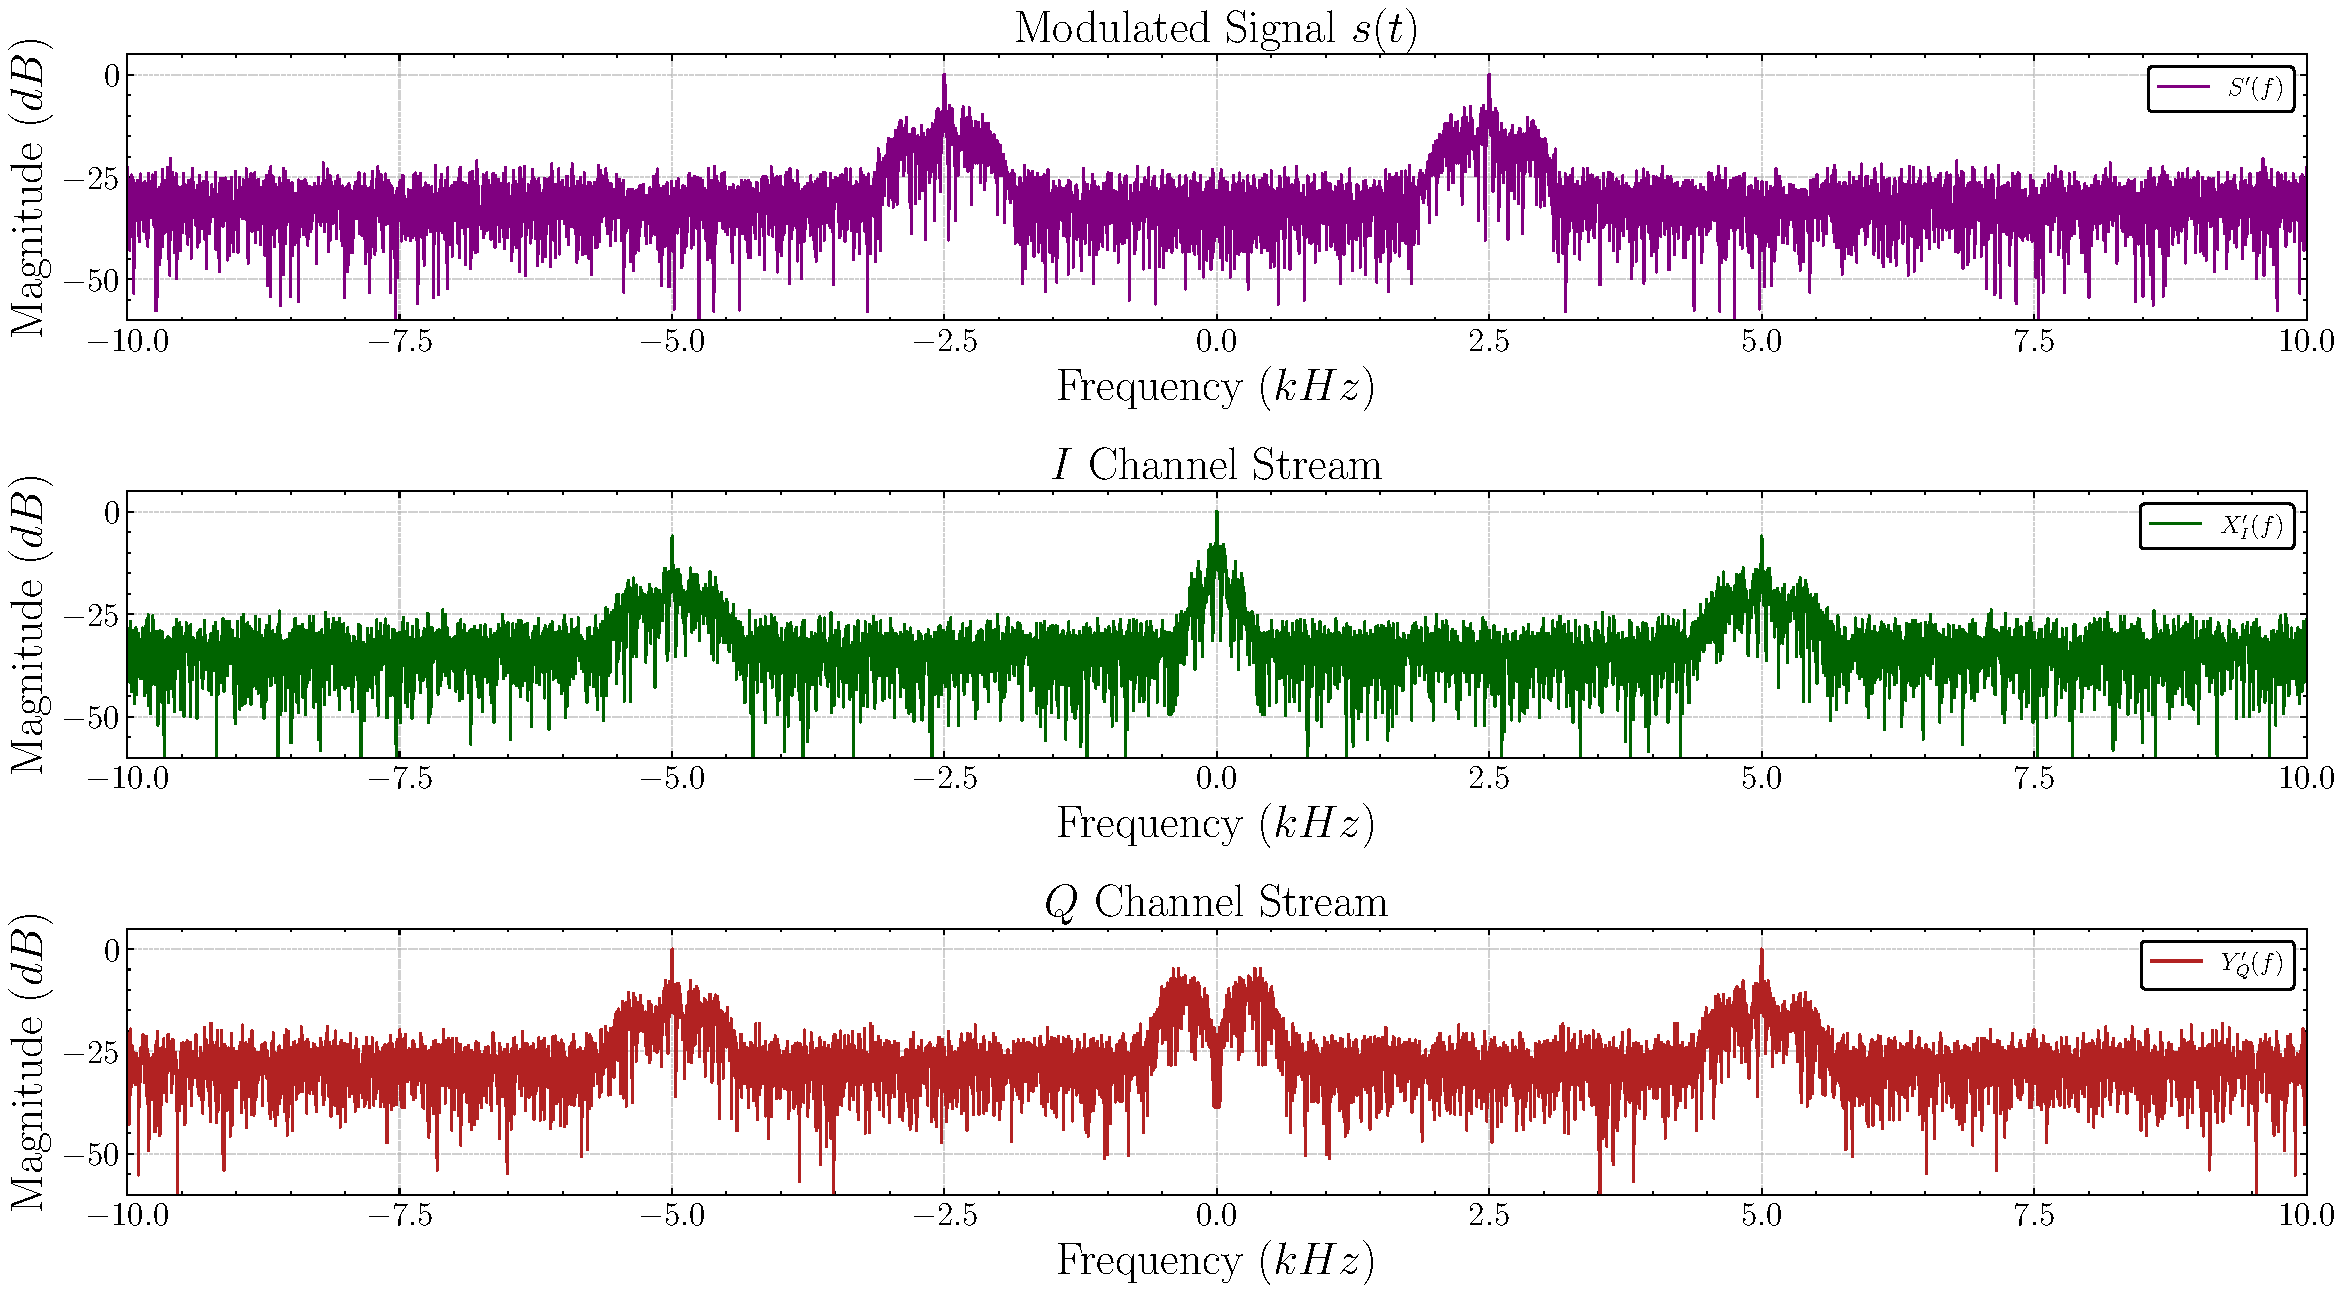
\includegraphics[width=\linewidth]{assets/cap3/receiver_demodulator_freq.pdf}
\end{figure}

\subsection{Filtragem}\label{sec:filtragem}

\begin{figure}[H]
	\centering
	\caption{Filtragem passa baixa dos canais $I$ e $Q$}\label{fig:receiver_lpf}
	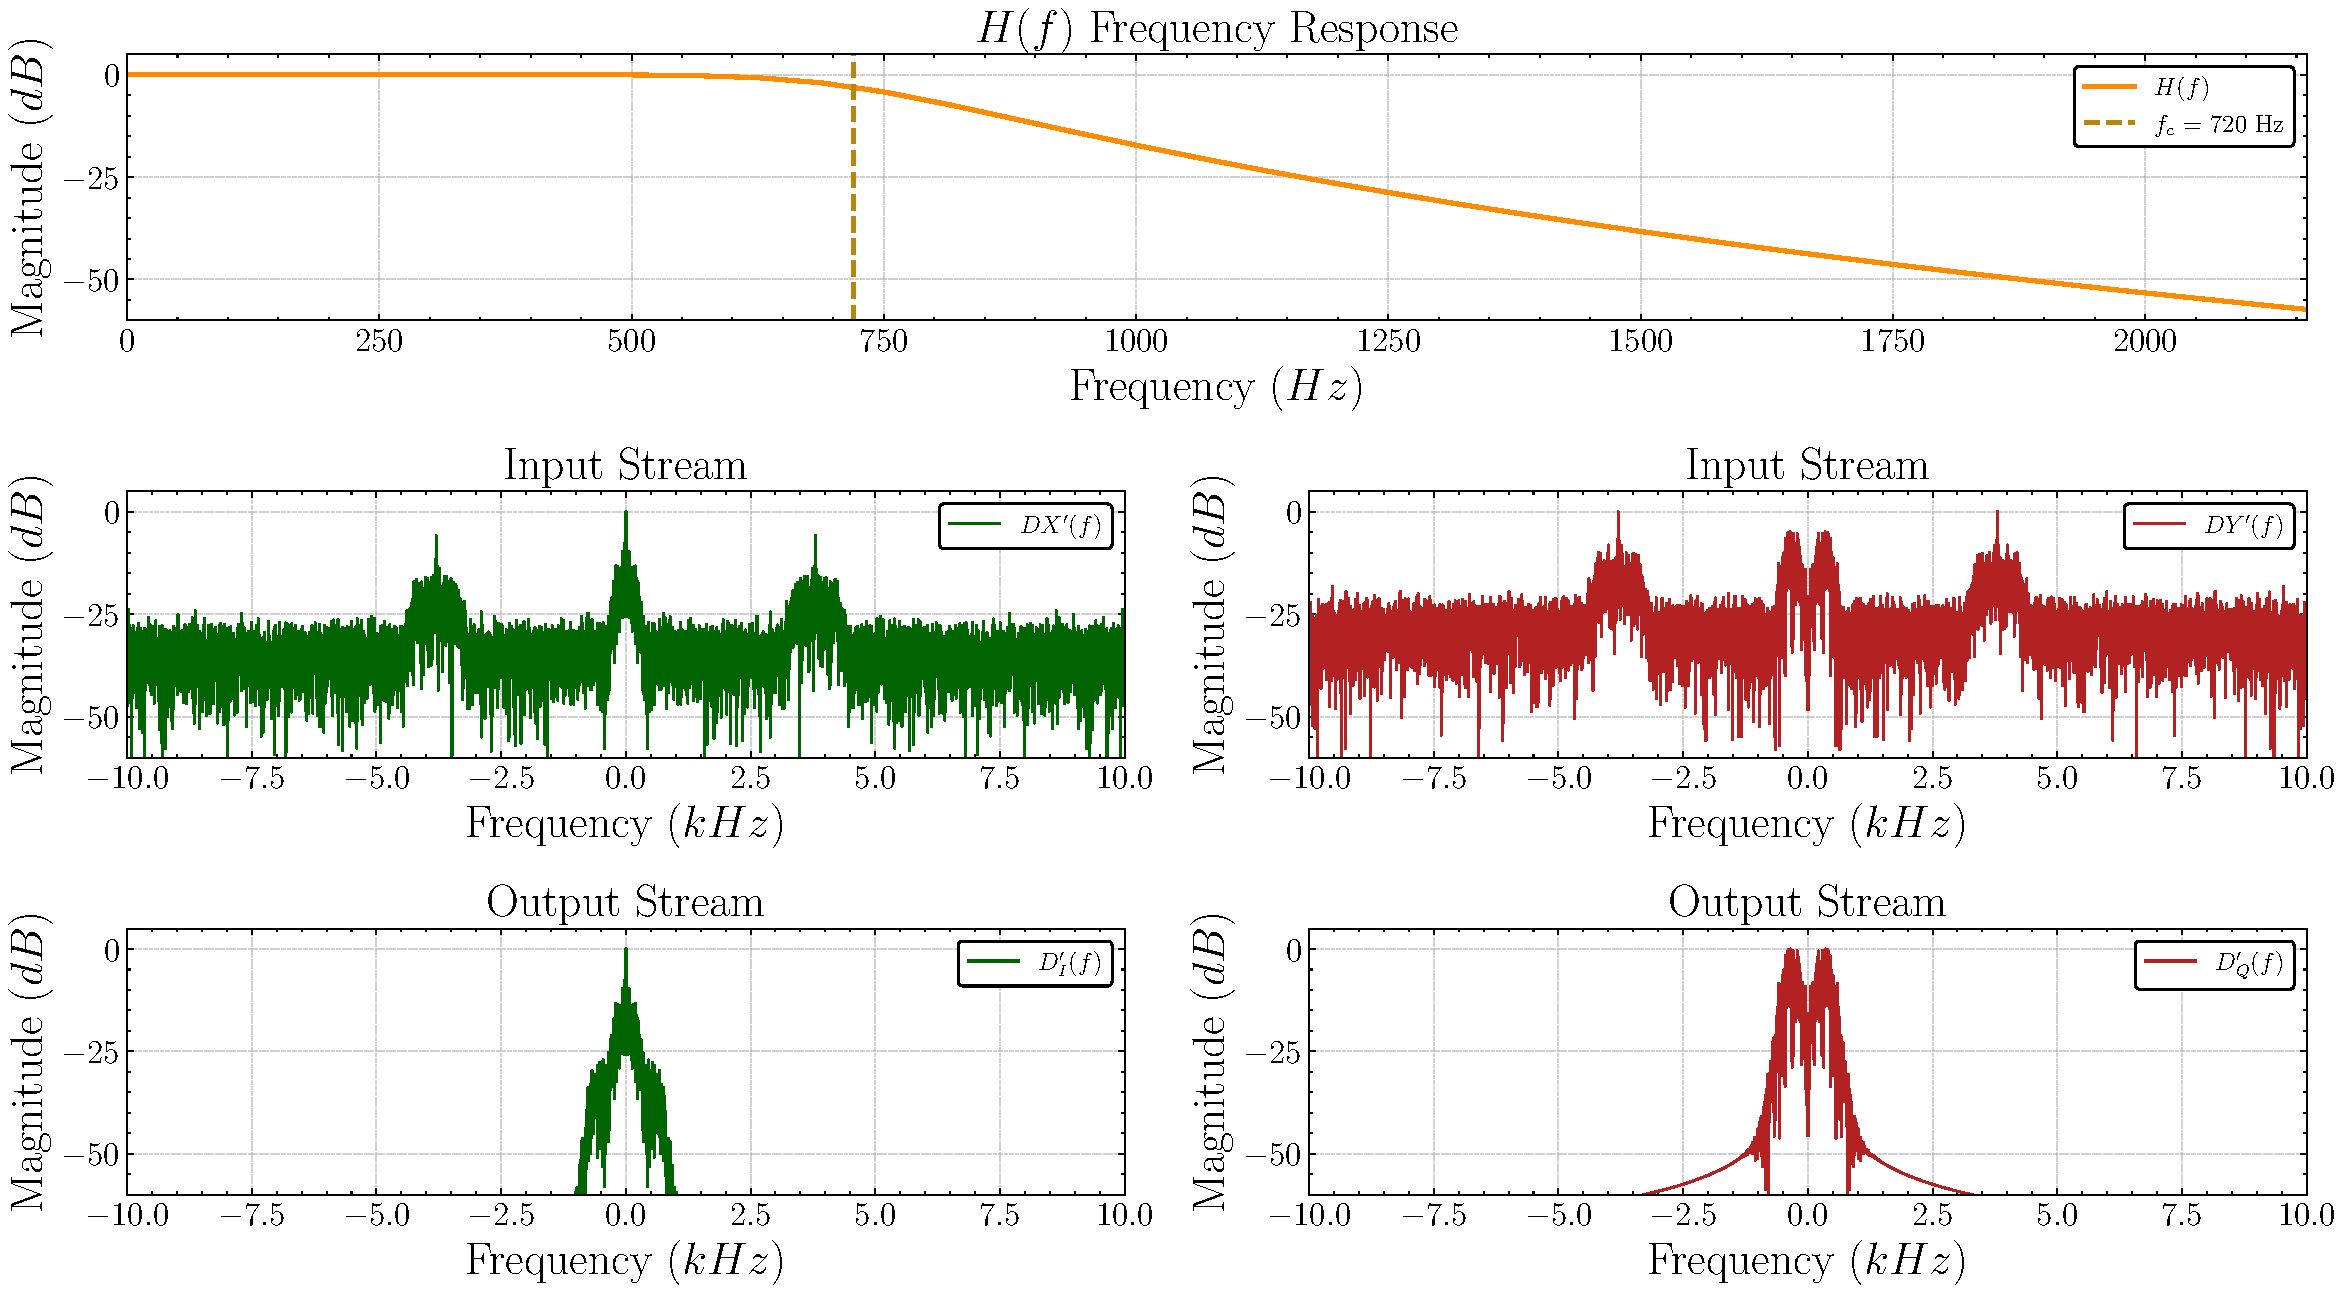
\includegraphics[width=\linewidth]{assets/cap3/receiver_lpf_freq.pdf}
\end{figure}

\begin{figure}[H]
	\centering
	\caption{Filtragem casada dos canais $I$ e $Q$}\label{fig:receiver_matchedfilter}
	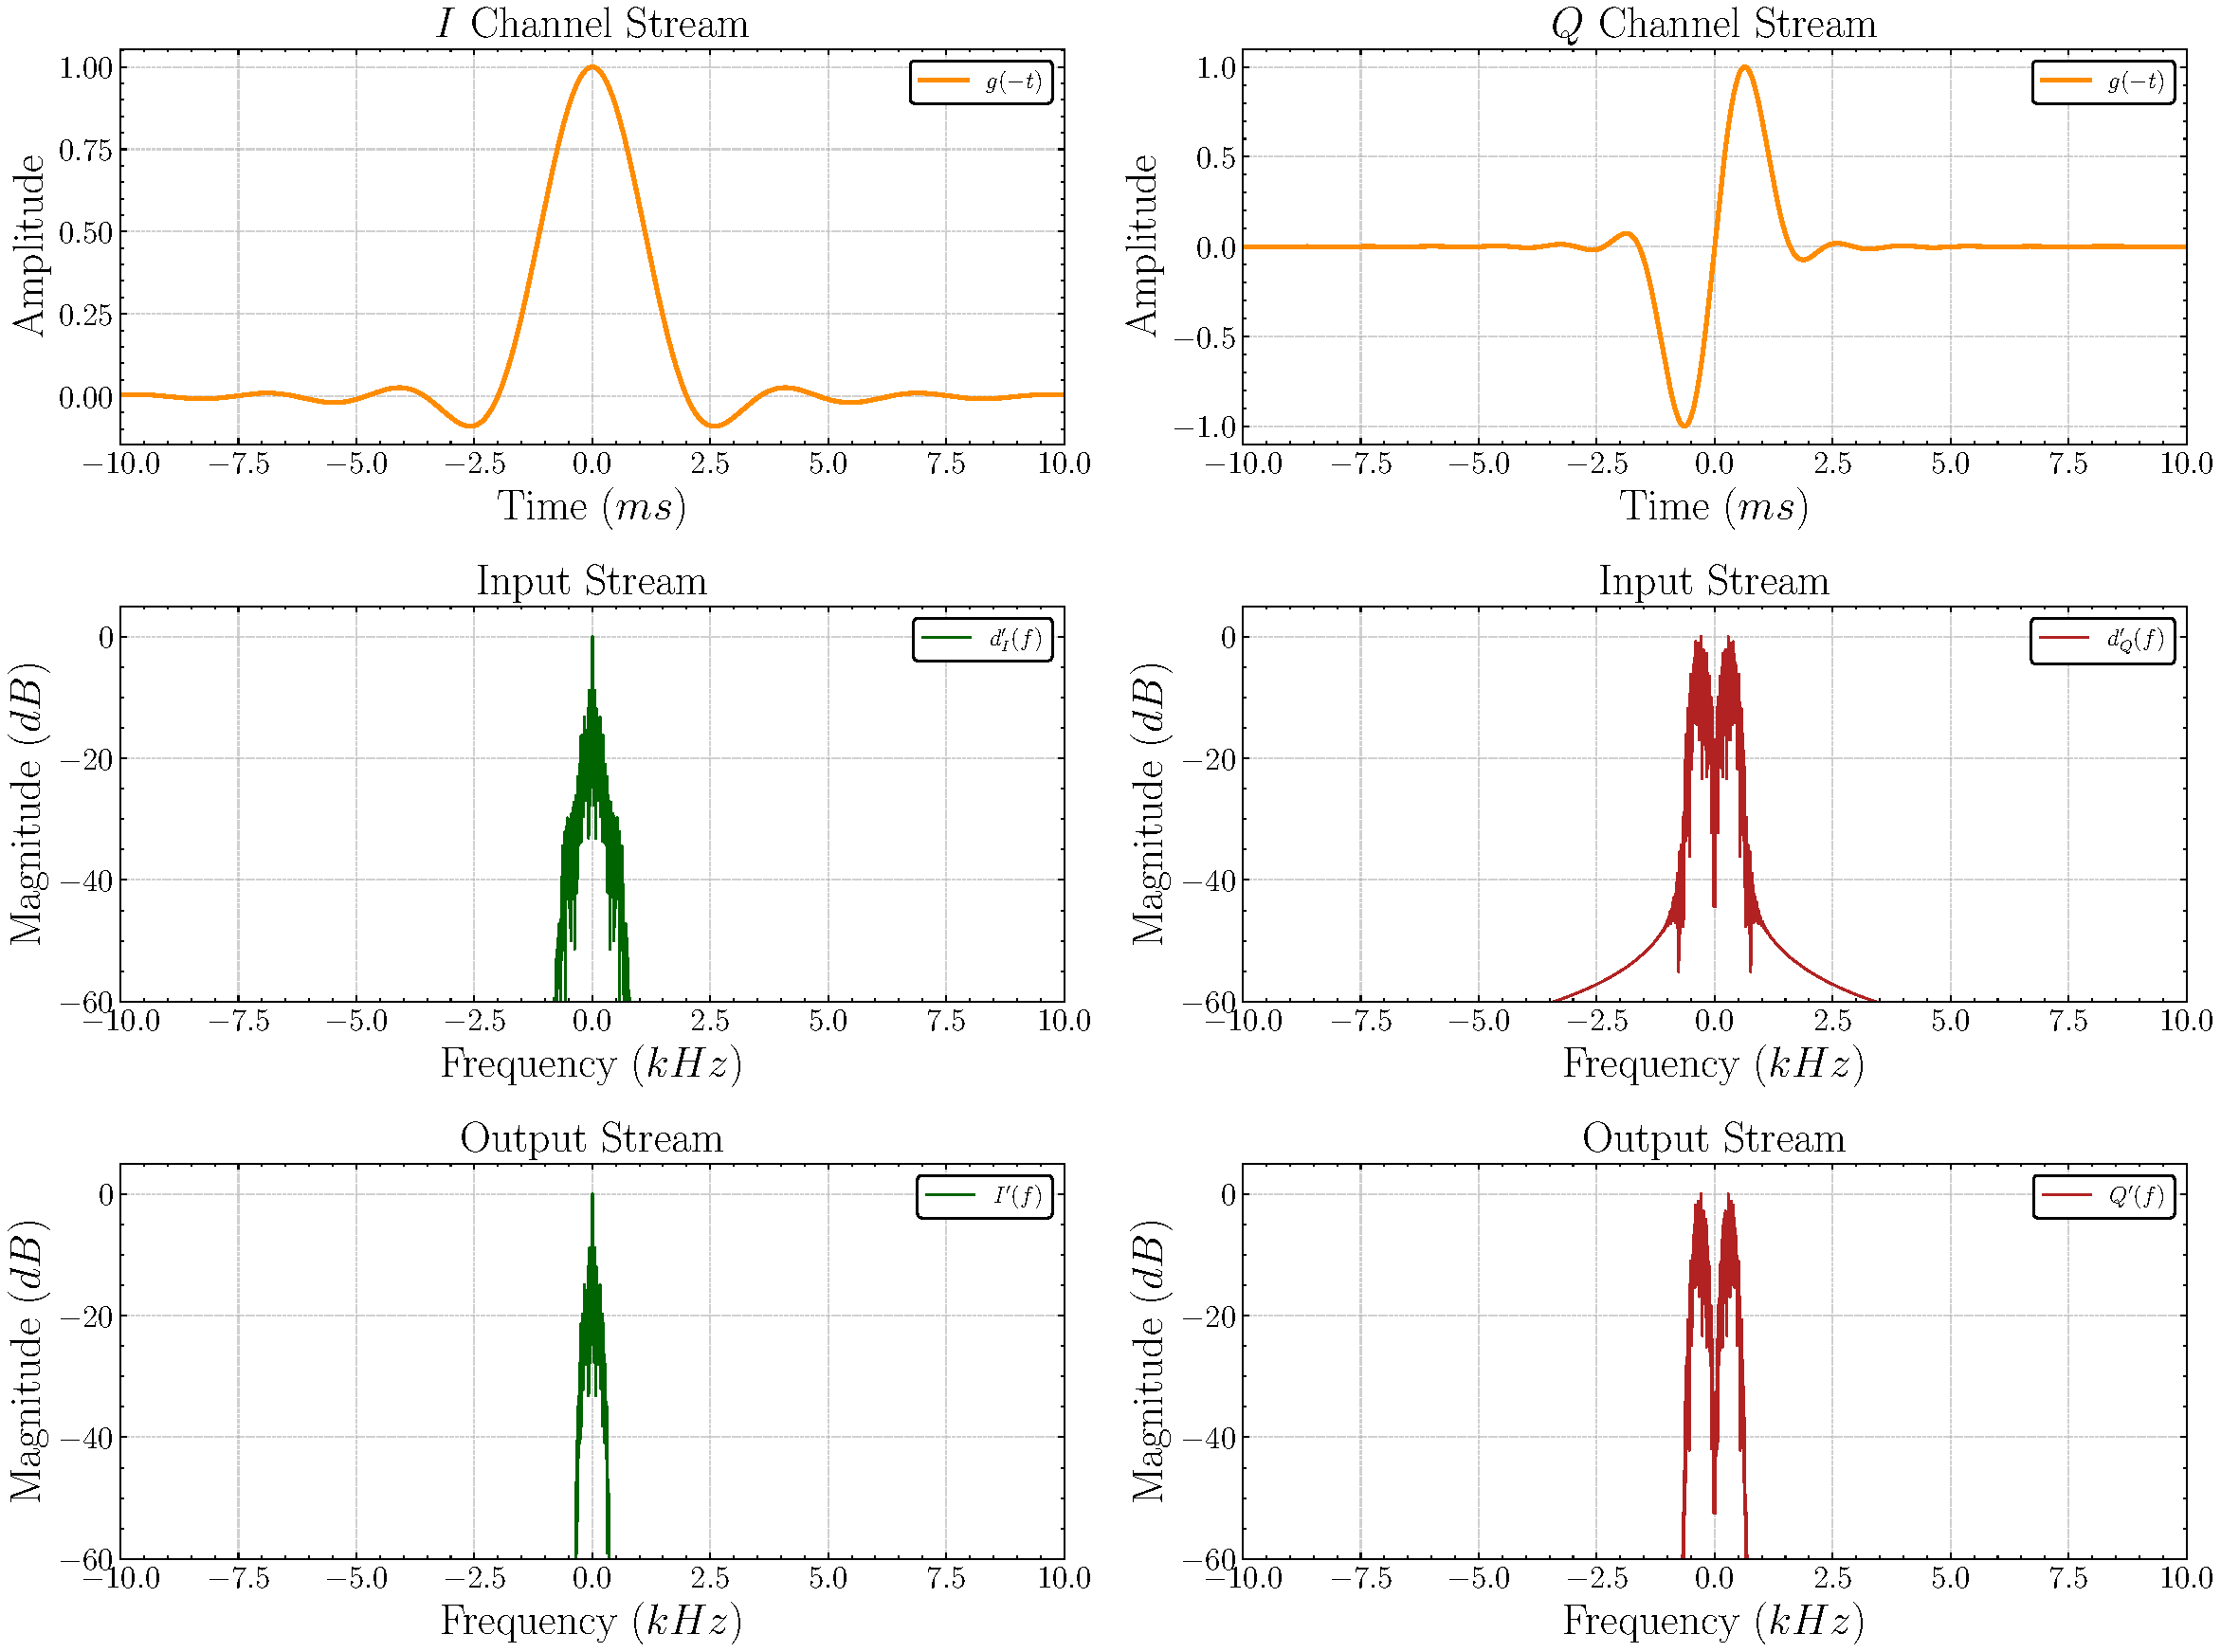
\includegraphics[width=\linewidth]{assets/cap3/receiver_mf_freq.pdf}
\end{figure}

\subsection{Sincronização de símbolos}\label{sec:sincronizacao}

\begin{figure}[H]
	\centering
	\caption{Diagrama de blocos para montagem do vetor de sincronismo}\label{fig:receiver_sync_diagram}
	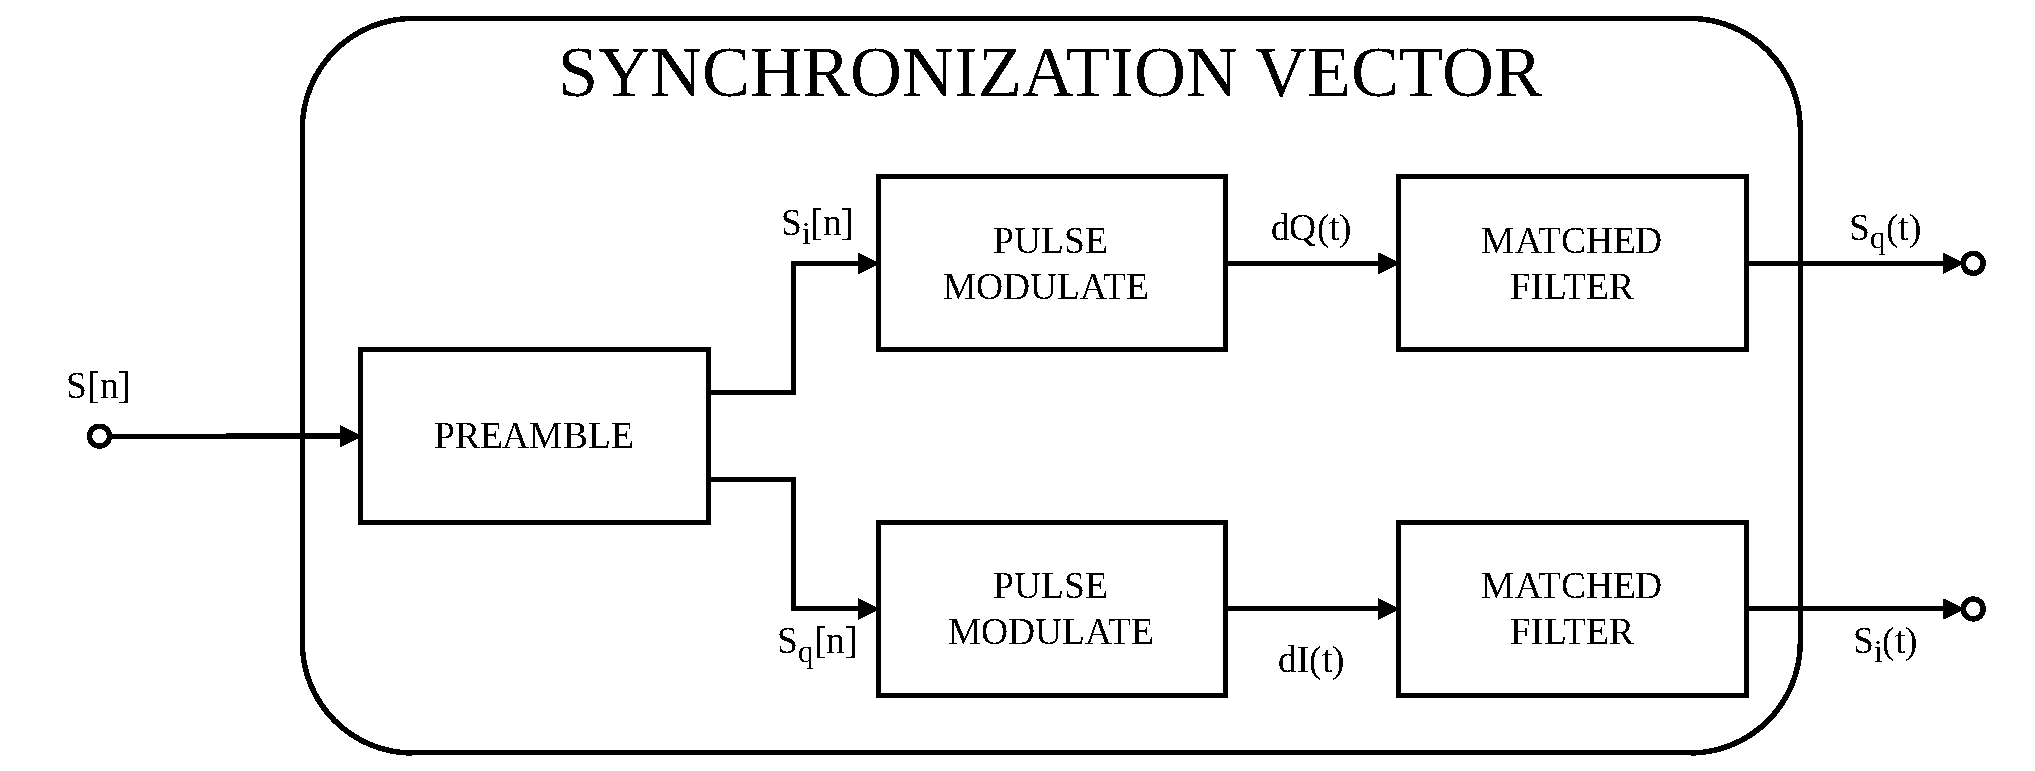
\includegraphics[width=\linewidth]{assets/diagrams/sync.pdf}
\end{figure}


\begin{figure}[H]
	\centering
	\caption{Vetor de amostras esperadas para sincronismo com $I$ e $Q$}\label{fig:receiver_sync_word}
	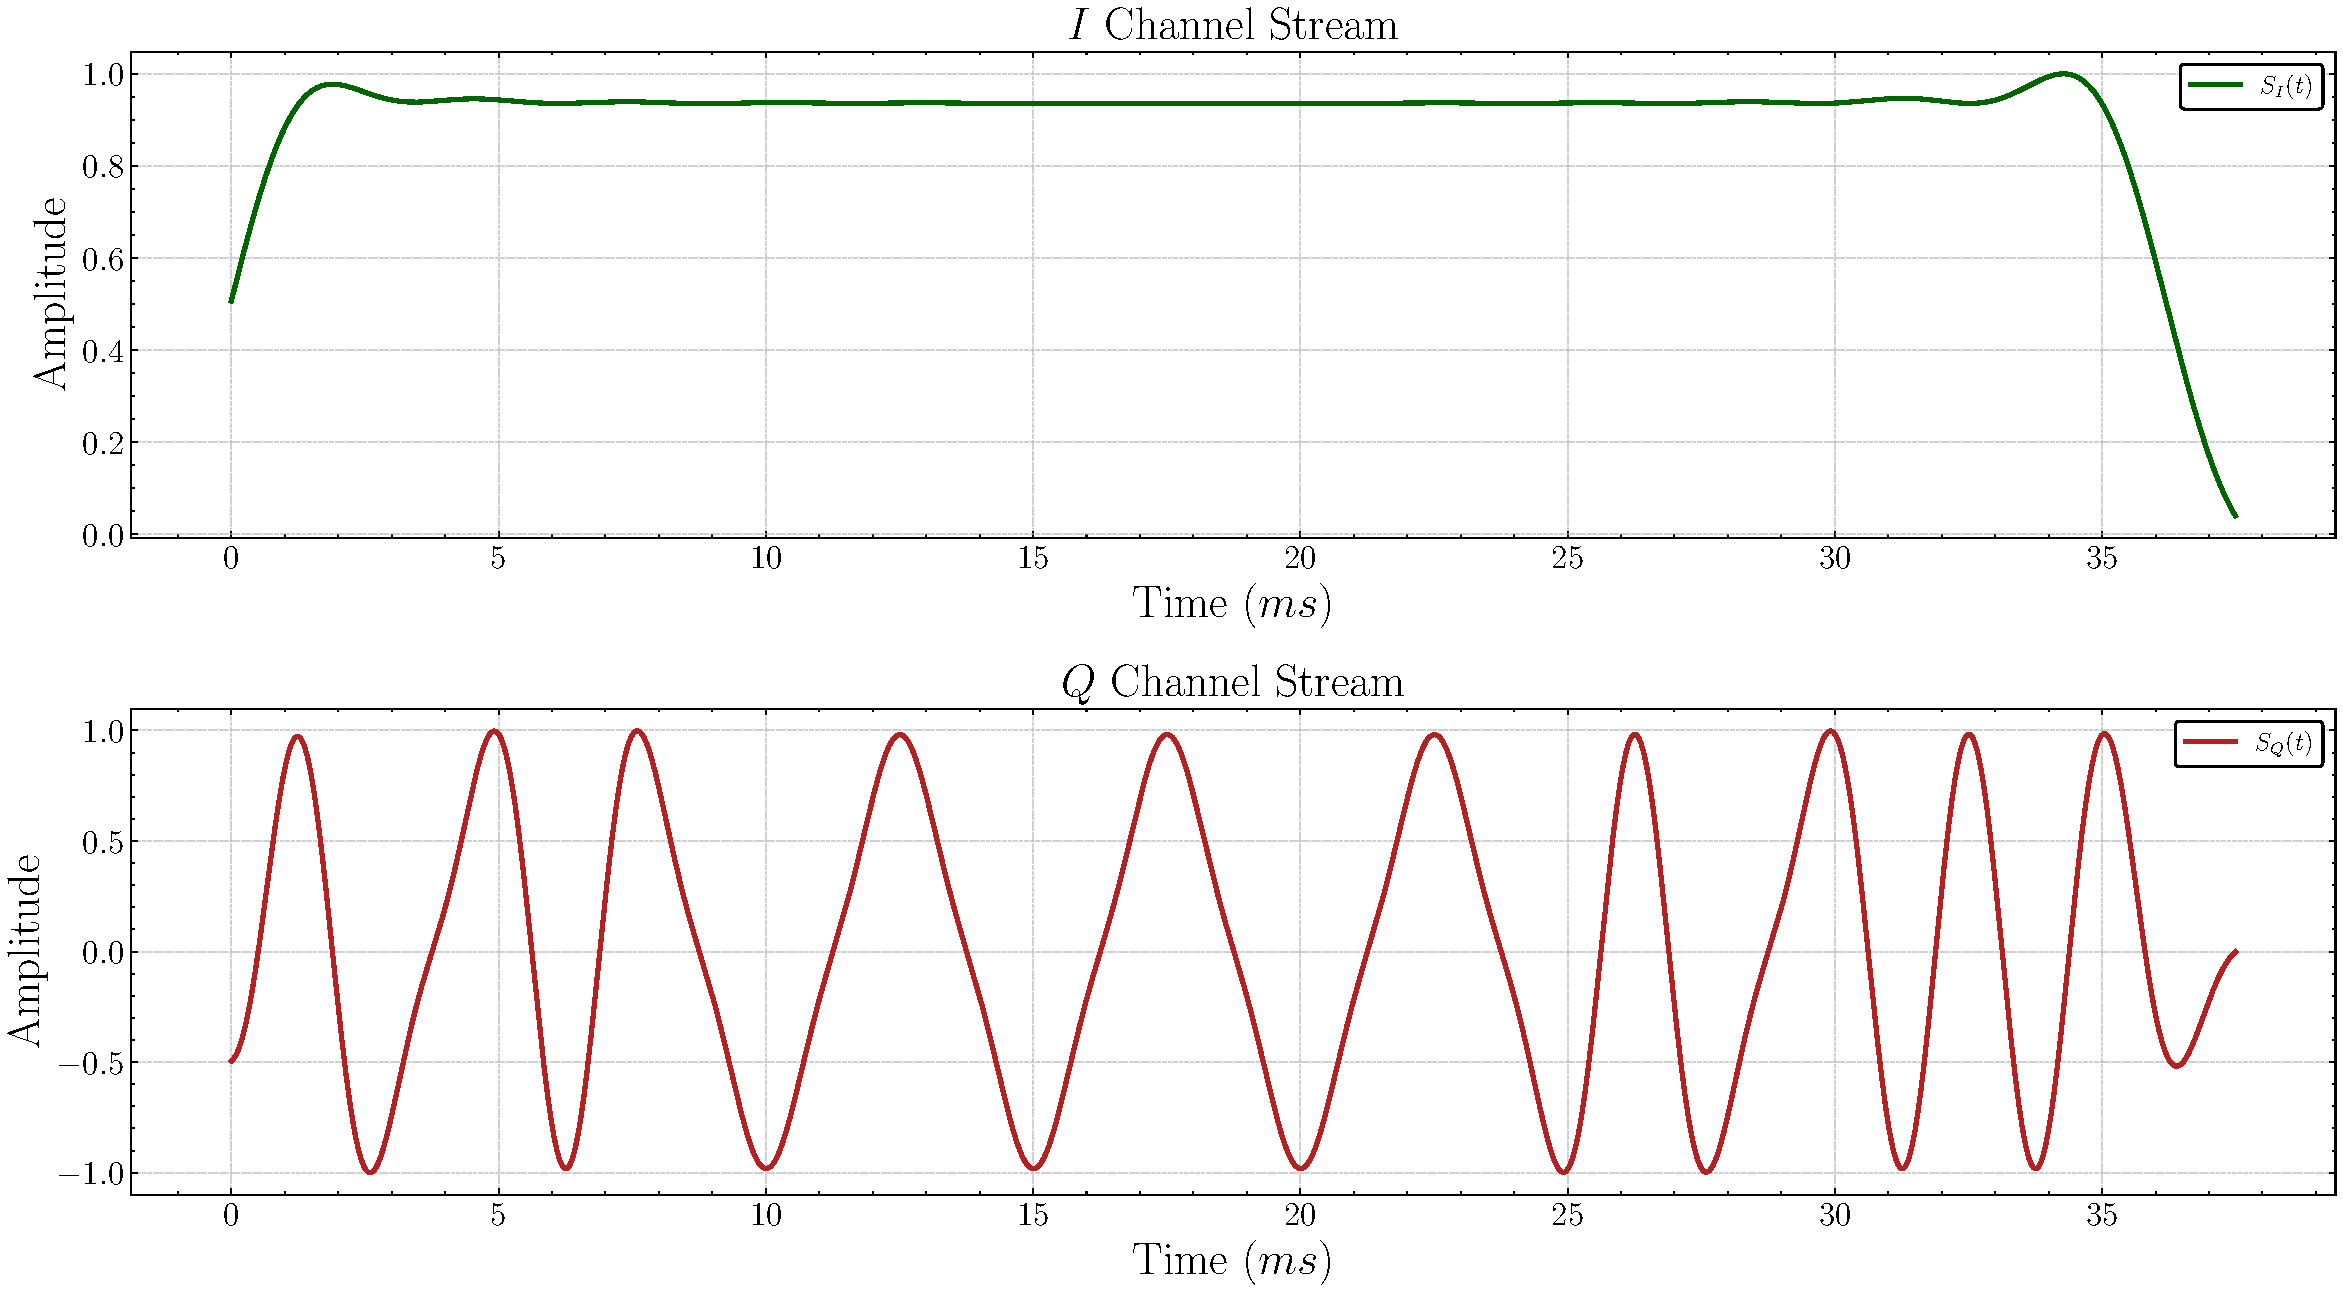
\includegraphics[width=\linewidth]{assets/cap3/example_synchronizer_word.pdf}
\end{figure}

\begin{figure}[H]
	\centering
	\caption{Módulo de correlação entre $I$ e $Q$ e vetor de sincronismo}\label{fig:receiver_corr}
	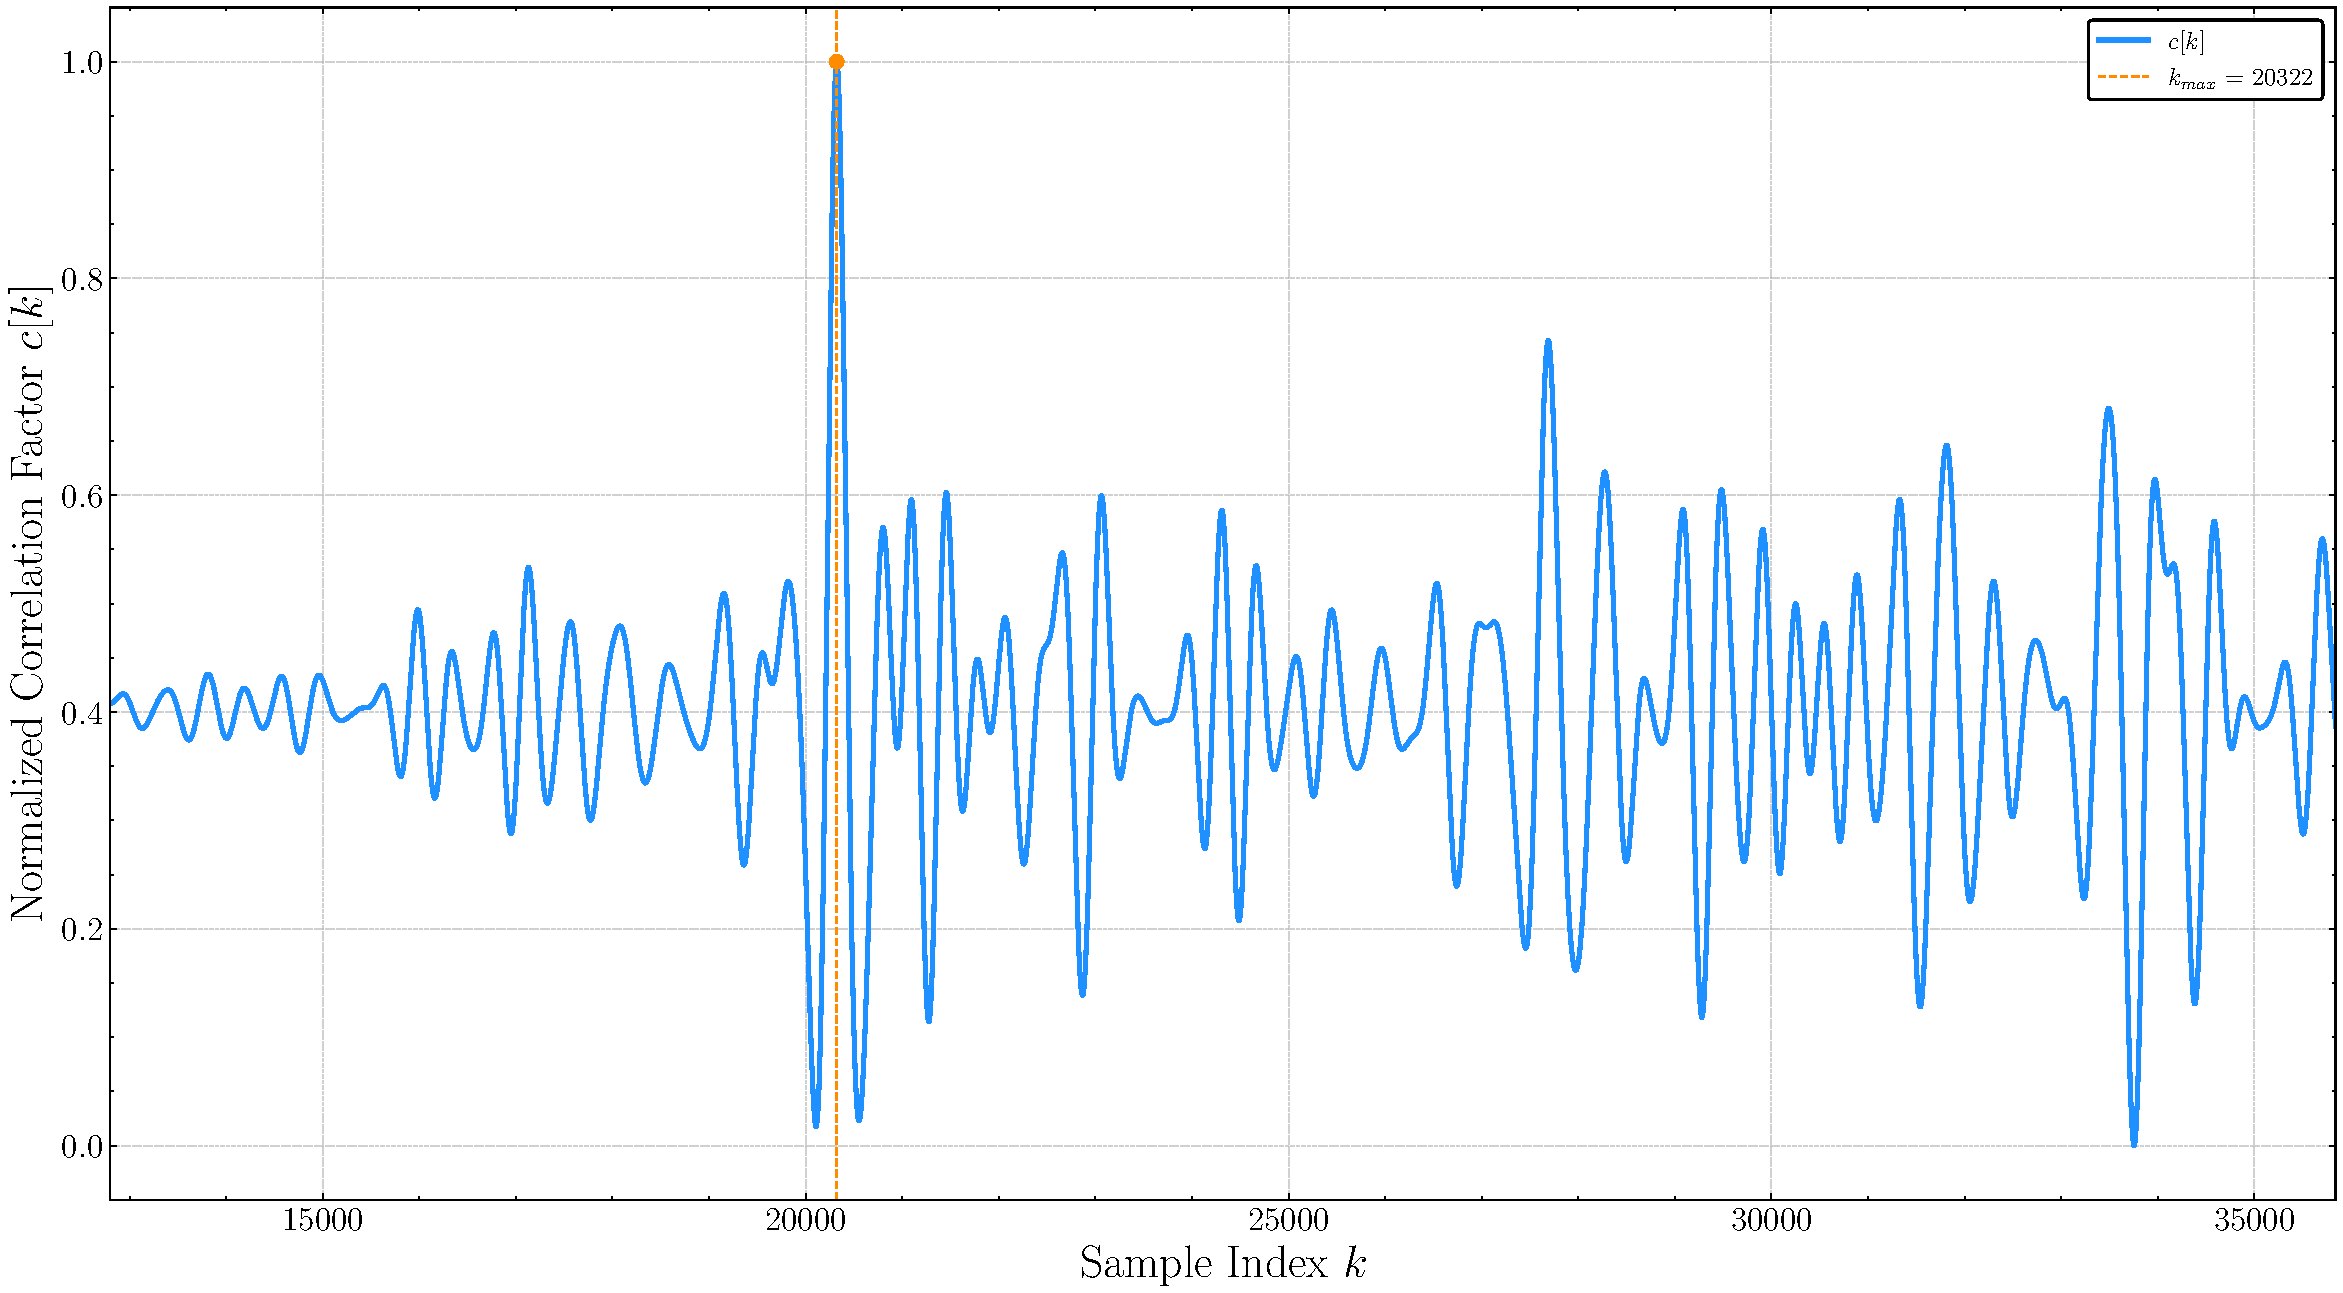
\includegraphics[width=\linewidth]{assets/cap3/receiver_sync_corr.pdf}
\end{figure}

\begin{figure}[H]
	\centering
	\caption{Sicronização de $I$ e $Q$ com vetor de sincronismo}\label{fig:receiver_sync}
	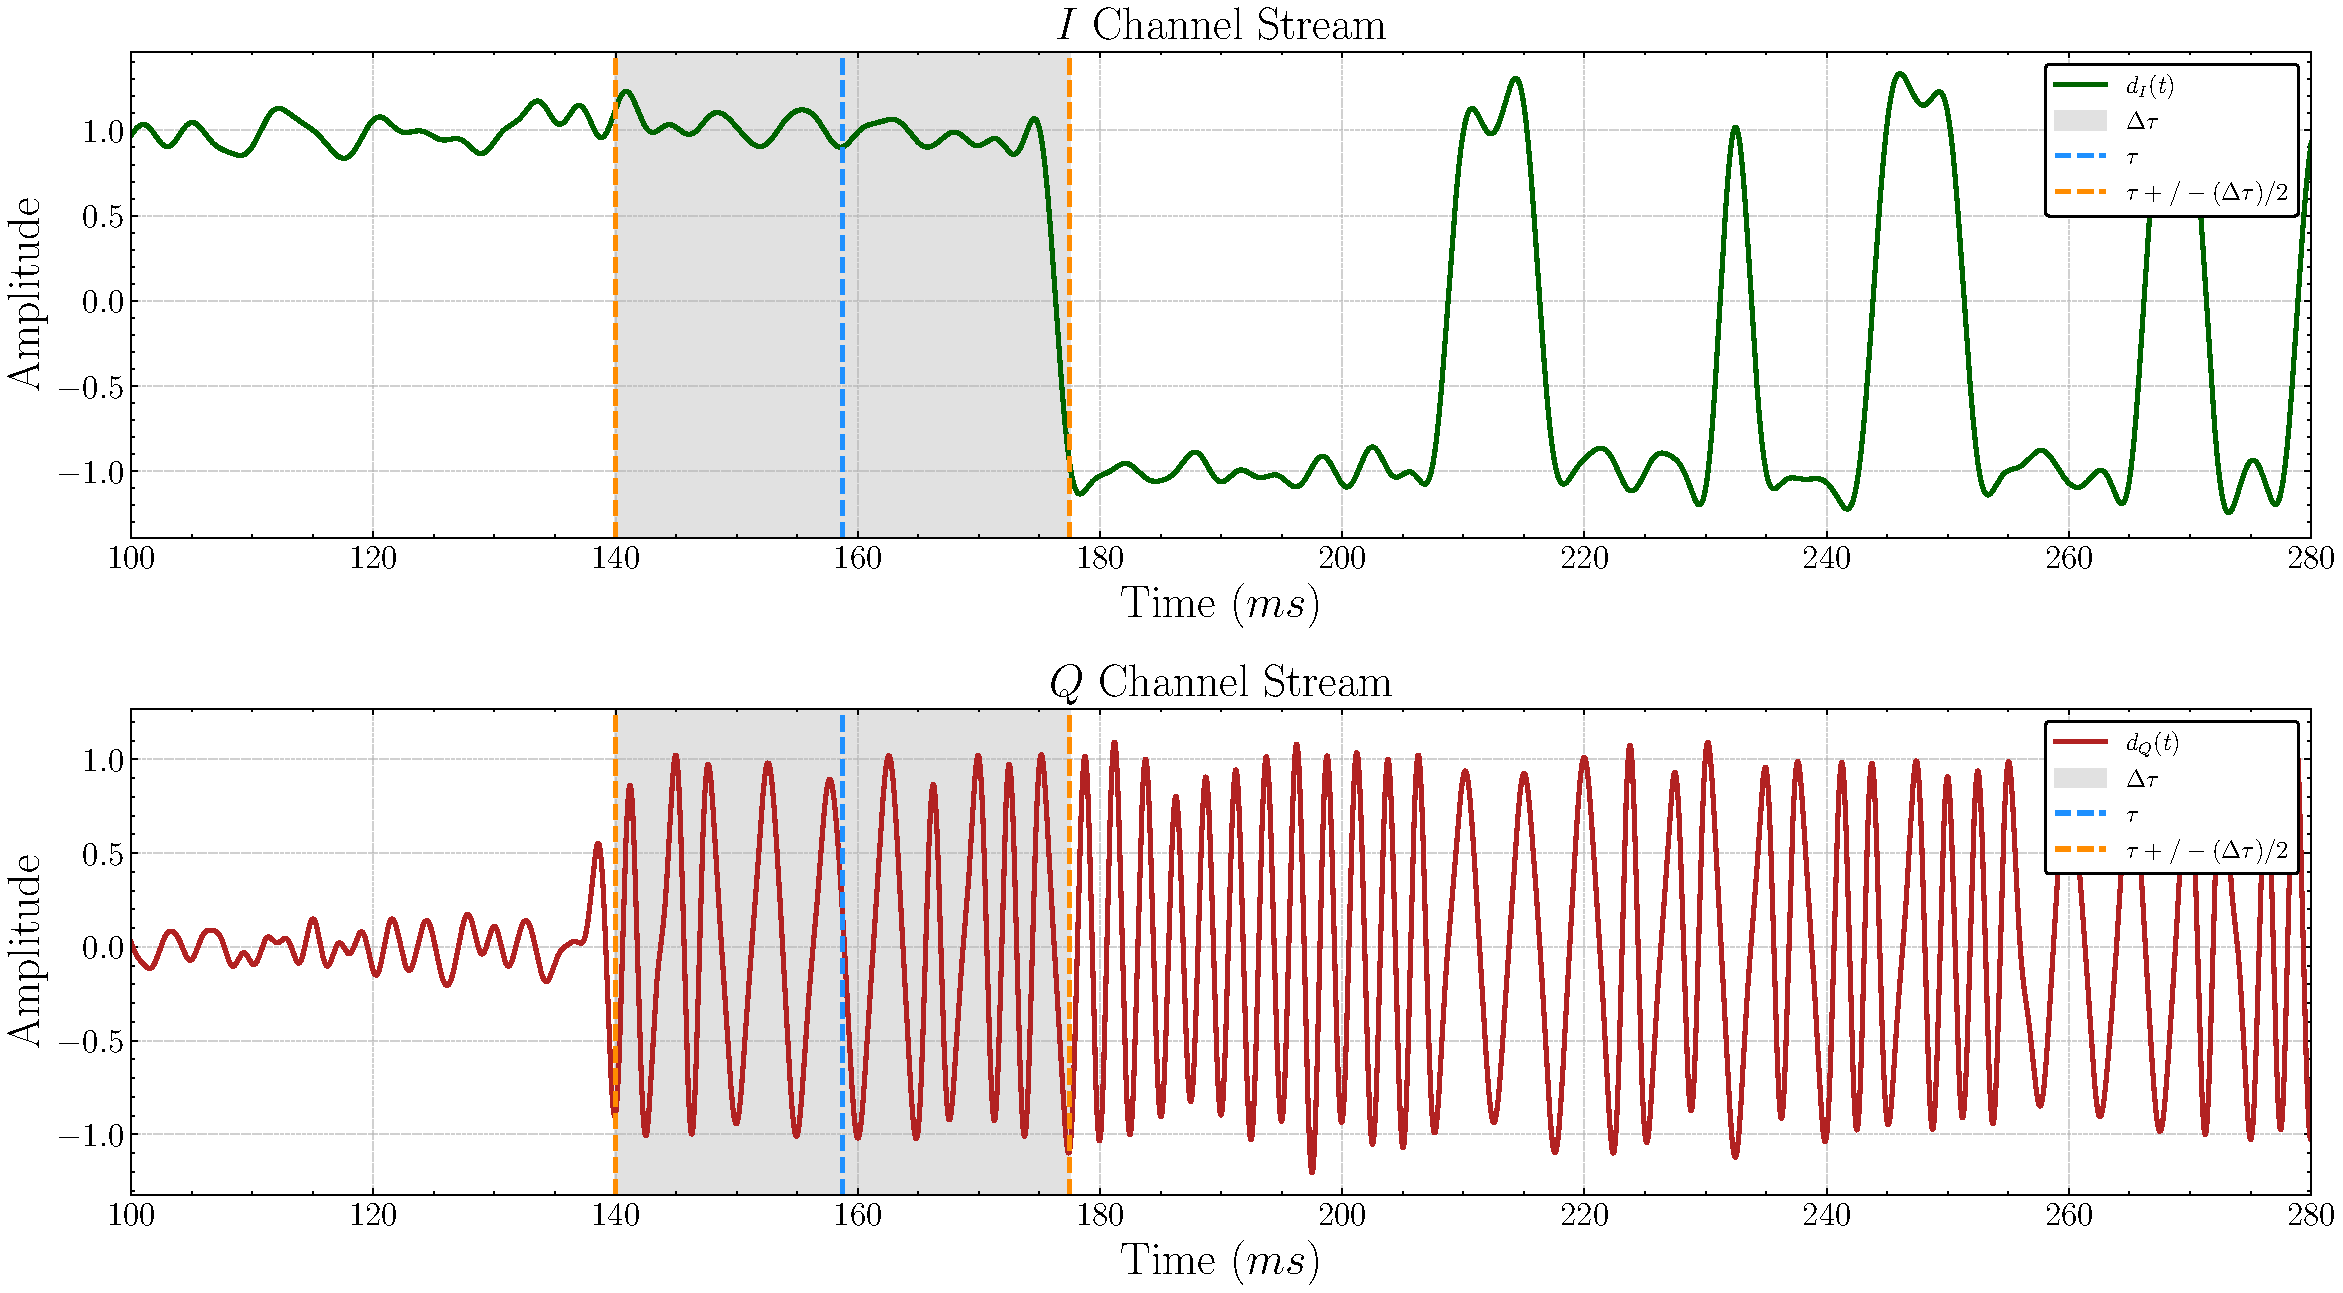
\includegraphics[width=\linewidth]{assets/cap3/receiver_sync_time.pdf}
\end{figure}


\subsection{Decisão de símbolos}\label{sec:decisao_simbolos}

\begin{figure}[H]
	\centering
	\caption{Amostragem dos canais $I$ e $Q$ em $T_b$ a partir de \gls{tau}}\label{fig:receiver_sampler}
	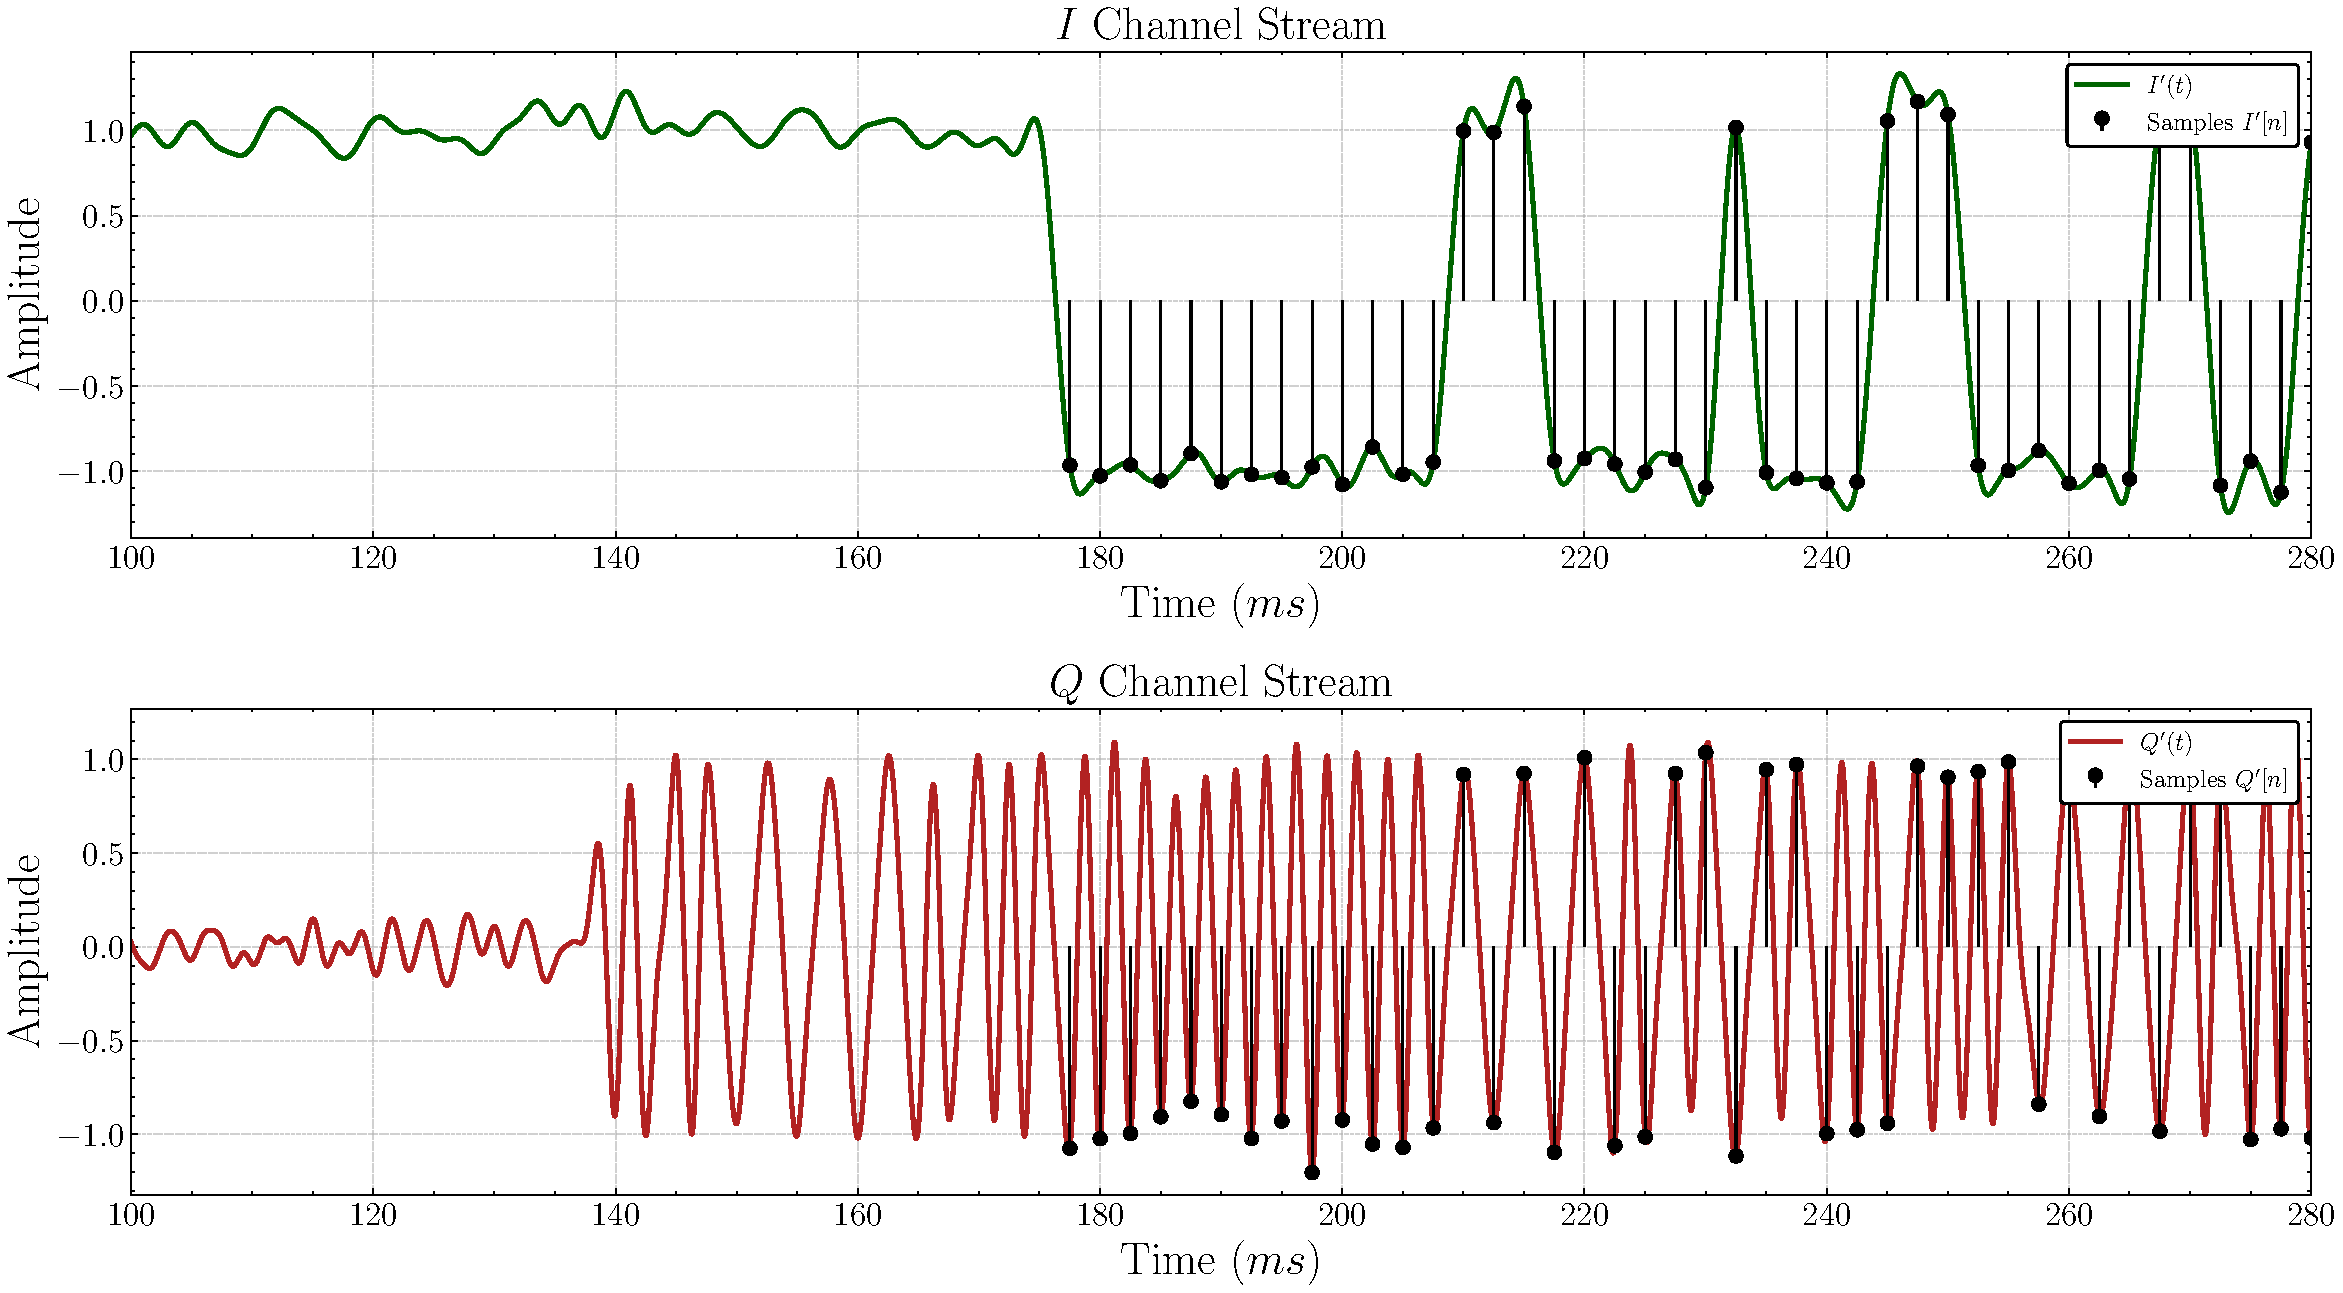
\includegraphics[width=\linewidth]{assets/cap3/receiver_sampler_time.pdf}
\end{figure}

\begin{figure}[H]
	\centering
	\caption{Constelação dos canais $I$ e $Q$ filtrados e amostrados}\label{fig:receiver_const}
	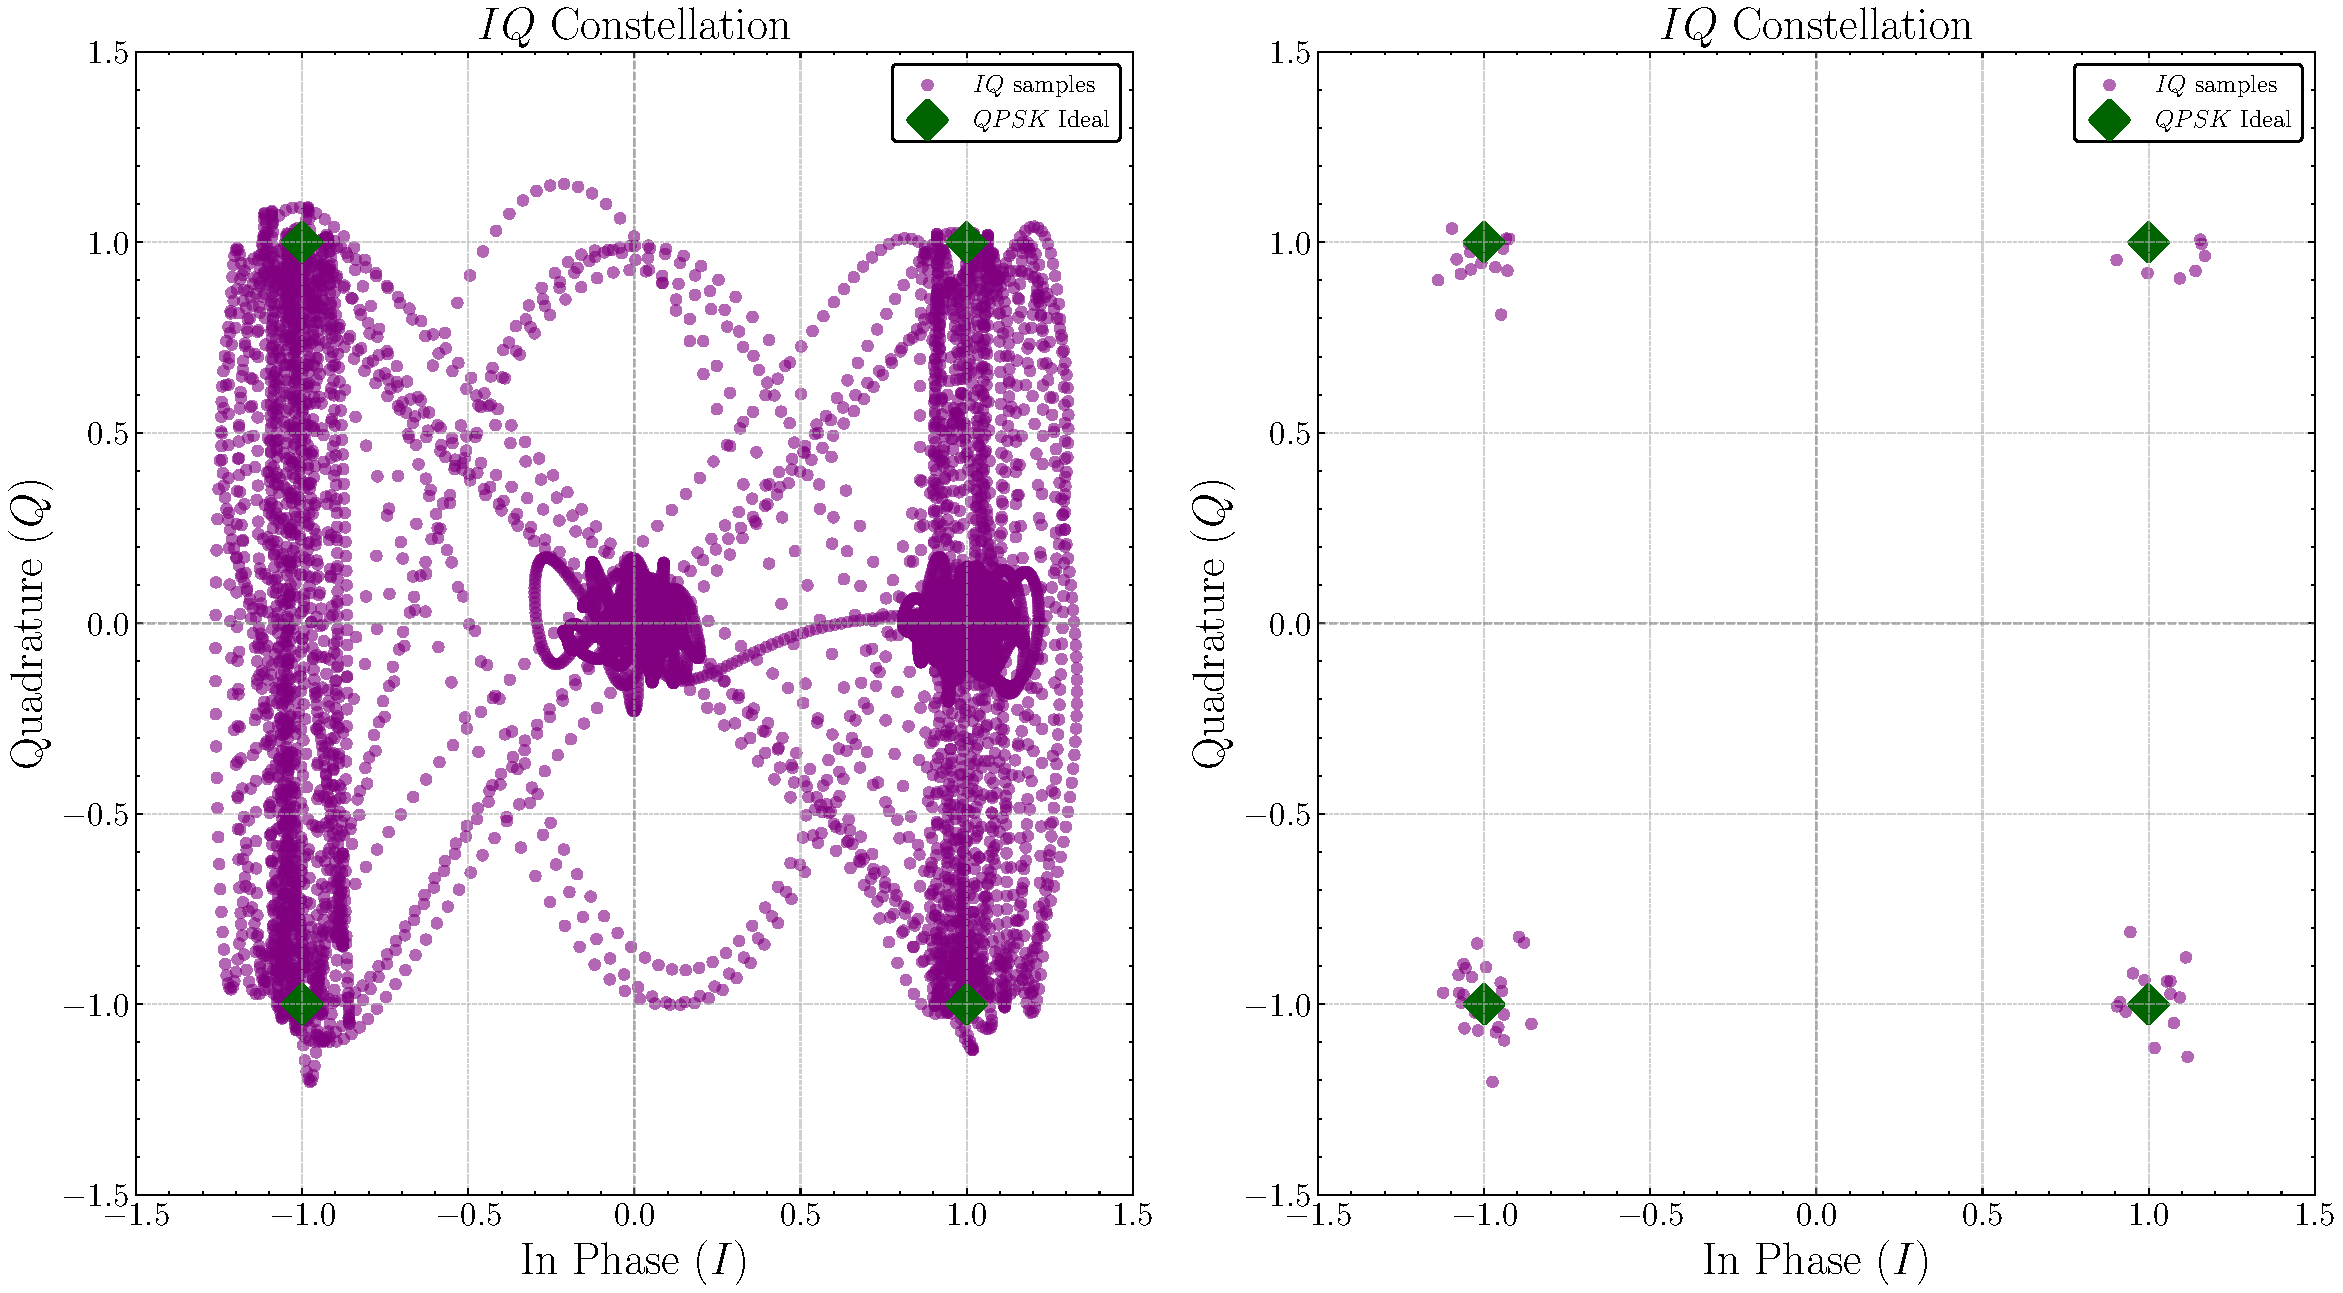
\includegraphics[width=\linewidth]{assets/cap3/receiver_sampler_const.pdf}
\end{figure}

\subsection{Recuperação do Datagrama}\label{sec:decodificacao_convolucional}

\begin{figure}[H]
	\centering
	\caption{Decodificação convolucional dos canais $I$ e $Q$}\label{fig:receiver_conv}
	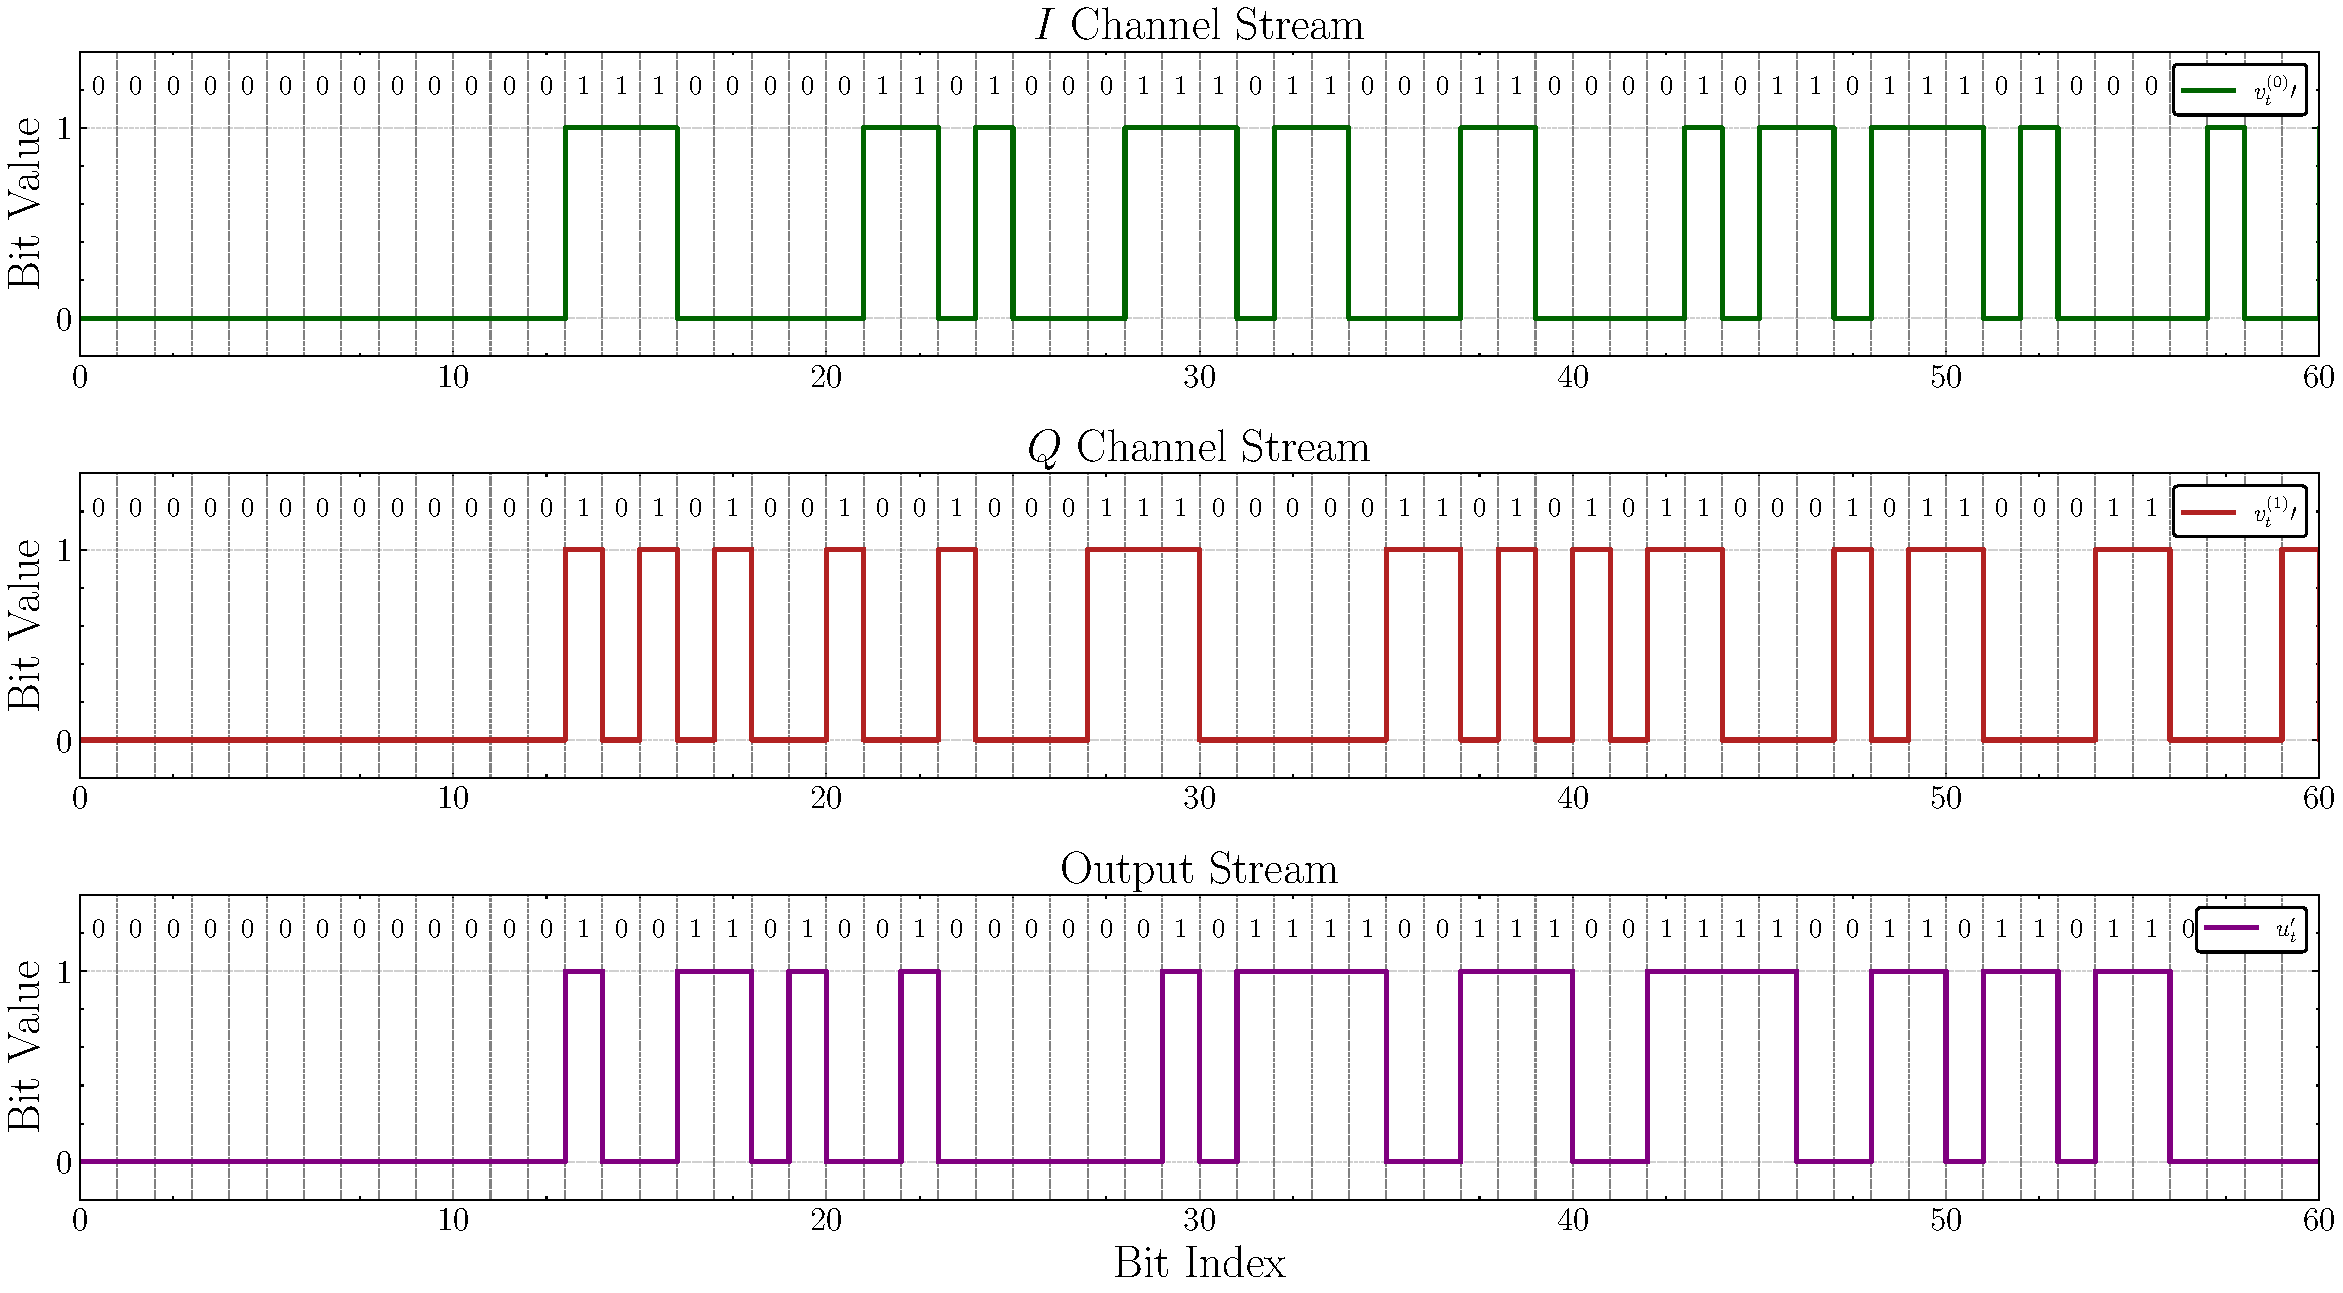
\includegraphics[width=\linewidth]{assets/cap3/receiver_conv_time.pdf}
\end{figure}